% !TeX root = main.tex
\documentclass{ctuthesis}
\usepackage{float}
\usepackage{multirow}
\usepackage{siunitx}
\usepackage{amsmath}
\usepackage{amssymb}
\usepackage{pgfplots}
\usepackage{filecontents}
\usepgfplotslibrary{statistics}
\usepackage{pgfplotstable}
\usepackage{tikz}
\usepackage{svg}
\setsvg{inkscape={"C:/Program Files/Inkscape/bin/inkscape.com"}}

\usetikzlibrary{spy,shadows}
\tikzset{spy using overlaysshadow/.style={
    spy scope={#1,
         every spy on node/.style={
            circle,
            fill, fill opacity=0.2, text opacity=1
             },
         every spy in node/.style={
                 circle, circular drop shadow,
                 fill=white, draw, ultra thick, cap=round
            }
        }
    }
}


\ctusetup{
	% preprint = \ctuverlog,
%	mainlanguage = english,
	titlelanguage = czech,
	mainlanguage = czech,
	otherlanguages = {slovak,english},
	title-czech = {Systém pro neinvazivní měření hemodynamických parametrů},
	title-english = {System for non-invasive measurement of hemodynamic parameters},
	%subtitle-czech = {Cesta do tajů kdovíčeho},
	%subtitle-english = {Journey to the who-knows-what wondeland},
	doctype = B,
	faculty = F3,
	department-czech = {Katedra teorie obvodů},
	department-english = {Department of circuit theory},
	author = {Daniel Klamrt},
	supervisor = {doc. Ing. Vratislav Fabián, Ph.D},
	supervisor-address = {Praha, Technická 1902/2, \\ místnost: B2-36},
	fieldofstudy-english = {Medical electronics and bioinformatics},
	fieldofstudy-czech = {Lékařská elektronika a bioinformatika},
	keywords-czech = {Hemodynamické parametry, Neinvazivní, Systém, Embedded system, Rychlost šíření pulzní vlny, Analýza pulzní vlny, Oscilometrická metoda, Měření krevního tlaku, Suprasystolický tlak},
	keywords-english = {Hemodynamic parameters, Noninvasive, System, Embedded system, Pulse Wave Velocity, Pulse Wave Analysis, Oscilometric method, Blood Pressure measurement, Suprasystolic pressure},
	day = 25,
	month = 4,
	year = 2023,
	specification-file = {zadani_prace.pdf},
	front-specification = true,
%	front-list-of-figures = false,
%	front-list-of-tables = false,
	% monochrome = true,
%	layout-short = true,
}

\ctuprocess

\begin{thanks}
	Tímto chci poděkovat svému vedoucímu práce doc. Ing. Vratislavu Fabiánovi, Ph.D. za odborné vedení a poskytnutí prostředků pro realizaci systému. Firmě BTL Medical Technologies s.r.o za odborný náhled a poskytnutí strojů pro sestavení tvořeného systému a kolegům, kteří se podíleli na vývoji a výzkumu prvků tohoto systému. 
\end{thanks}

\begin{declaration}
Prohlašuji, že jsem předloženou práci vypracoval samostatně a že jsem uvedl veškeré použité informační zdroje v souladu s Metodickým pokynem o dodržování etických principů při přípravě vysokoškolských závěrečných prací.


V Praze, \ctufield{day}.~\monthinlanguage{title}~\ctufield{year}
\end{declaration}

\begin{abstract-english}
The bachelor's thesis deals with the design and implementation of a system for sensing blood pressure pulsations using an arm cuff, the measured parameters include pulse wave velocity, central aortic pressure and blood pressure.
The first part is focused on a theoretical description of hemodynamic parameters and description of devices for measuring hemodynamic parameters of the bloodstream determined non-invasively using pulse wave analysis. In the next part is the hardware design and documentation of the system. This is followed by a description of the pneumatic part, the implementation of the printed circuit board and the technical parameters of the system. 
Finally, the measured pressure pulsations of the volunteer at suprasystolic pressure $200 \ mmHg$ and $275 \ mmHg$ are shown.
\end{abstract-english}

\begin{abstract-czech}
Bakalářská práce se zabývá návrhem a realizací systému pro snímání tlakových pulzací pomocí pažní manžety. Mezi měřené hemodynamické parametry patří rychlost šíření pulzní vlny, centrální aortální tlak a krevní tlak. 
První část práce je zaměřena na teoretický popis hemodynamických parametrů a rešerši přístrojů pro měření hemodynamických parametrů krevního řečiště určovaných neinvazivně z tvaru tlakové křivky. V další části je hardwarový návrh a dokumentace systému. 
Na to navazuje popis pneumatické části, realizace desky plošného spoje a popis technických parametrů systému. Na zavěr jsou ukázány naměřené tlakové pulzace u dobrovolníka při suprasystolickém tlaku $200 \ mmHg$ a $275 \ mmHg$.
\end{abstract-czech}

\begin{document}

\maketitle


%% BEGIN

%Intro
\chapter{Úvod}
Cílem této bakalářské práce je návrh a realizace systému pro snímání tlakových pulzací pomocí pažní manžety. Systém je pojmenován CarDi (Cardiovascular Diagnostic), který měří krevní tlak, centrální aortální tlak a rychlost šíření pulzní vlny a splňuje normy
ISO 81060–1:2013 a ISO 81060–2:2013 \cite{cite:Validation}.
Práce navazuje na projekt TA ČR EPSILON 4, TH04010173 - Zařízení pro automatickou analýzu hemodynamických parametrů, který byl řešen na FEL, ČVUT v Praze v letech 2019 až 2021.


\par
První část seznámí čtenáře s měřením hemodynamických parametrů, a to zejména krevního tlaku a rychlosti šíření pulzní vlny. Dále pak na popis metod neinvazivního měření krevního tlaku, rešerši přístrojů dostupných na trhu zaměřených na neinvazivní měření rychlosti šíření pulzní vlny, jejich postup měření a ovládání z uživatelského hlediska.
\par
Další část se zaměří na návrh elektronického systému pro ovládání průběhu snímání a technickou dokumentaci.
\par
V části realizace systému CarDi je popsána deska plošného spoje, popis pneumatické části systému, parametry přístroje, charakteristiky analogově-digitálních převodníků pro tlakové sensory a měření pulzní tlakové vlny pomocí diferenčního sensoru tlaku.

%BloodPressure
%!TEX ROOT=main.tex
\chapter{Hemodynamické parametry}
Tato kapitola se zaměří na popis hemodynamických parametrů krevního řečiště.
\section{Krevní tlak}
Krevní tlak je veličina, která vyjadřuje velikost síly proudící krve, působící na stěnu cévy. Velikost krevního tlaku závisí na síle kontrakce srdce, množstvý krve uvnitř těla,
odporu cév a elasticitě stěny cév. Krevní tlak se uvadí ve dvou typech. Systolický tlak, který vyjadřuje působící sílu krve proti stěně artérie, při kontrakci srdce a diastolický tlak vyjadřuje
tlak, kdy srdce je v klidu mezi jeho činnosti. Krevní tlak se uvádí v jednotkách $mmHg$ milimetrů rtuti, co odpovídá $133.32
    \  Pa$. Jako normální lidský krevní tlak se považuje méně jak $120 \ mmHg$ systolického a měně jak  $80 \ mmHg$ diastolického tlaku.
\subsection{Centrální aortální tlak}
Centrální aortální tlak je tlak v aortě, do které krev putuje při kontrakci srdce. \par
Centrální aortální tlak je možno měřit neinvazivním způsobem, připevněním manžety na horní část ruky nebo zápěstí. Ze snímané tlakové křivky je
možné estimovat centrální aortální tlak.

\subsection{Střední arteriální tlak}
Střední arteriální tlak (MAP) je průměrná hodnota krevního tlaku v jednom srdečním cyklu.
\begin{figure}[H]
    \caption{Průběh tlakové křivky pro výpočet středního arteriálního tlaku}
    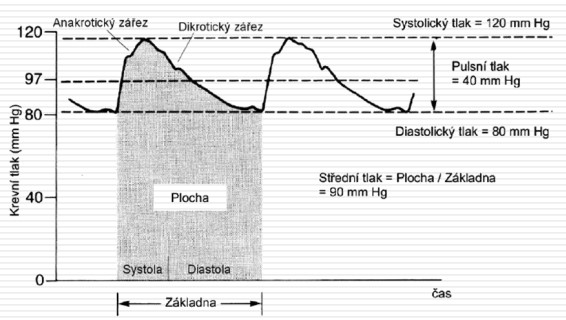
\includegraphics[width=1\textwidth]{pictures/map.jpg}
\end{figure}
Rovnice pro přesný výpočet je
\begin{equation}
    MAP = \frac{1}{T} \int_{t}^{t + T} BP(\tau) d\tau
\end{equation}
Rovnice pro aproximaci je
\begin{equation}
    MAP = DP + \frac{1}{3}(SP - DP)
\end{equation}
Kde $DP$ je diastolický tlak a $SP$ je systolický tlak.
\section{Metody měření krevního tlaku}
Metody měření tlaku můžou být invazivní nebo neinvazivní, manuální čí automatizované. Jedním k nejvíce používaných metod pro neinvazivní měření
krevního tlaku patří auskultační metoda, která používá rtuťového sphygmomanometeru a stetoskopu pro poslouchání krevní vlny. Další nejvíce používaná metoda je oscilometrická metoda.
\subsection{Oscilometrická metoda}
Oscilometrická metodu měření tlaku využívá navrhovaný systém CarDi. Metoda spočívá v měření objemové pulzace v tepnách přenášející se přes manžetu do přístroje, ve kterém se vyhodnocují.
Amplituda těchto pulzací je závislá na rozdílu tlaku uvnitř a vně tepny, tzv. transmurální tlak. Největší amplituda při je při nulovém transmurální tlaku, to je při hodnotě středního arteriální tlaku.

\begin{figure}[H]
    \caption{Graf oscilometrických pulzací}
    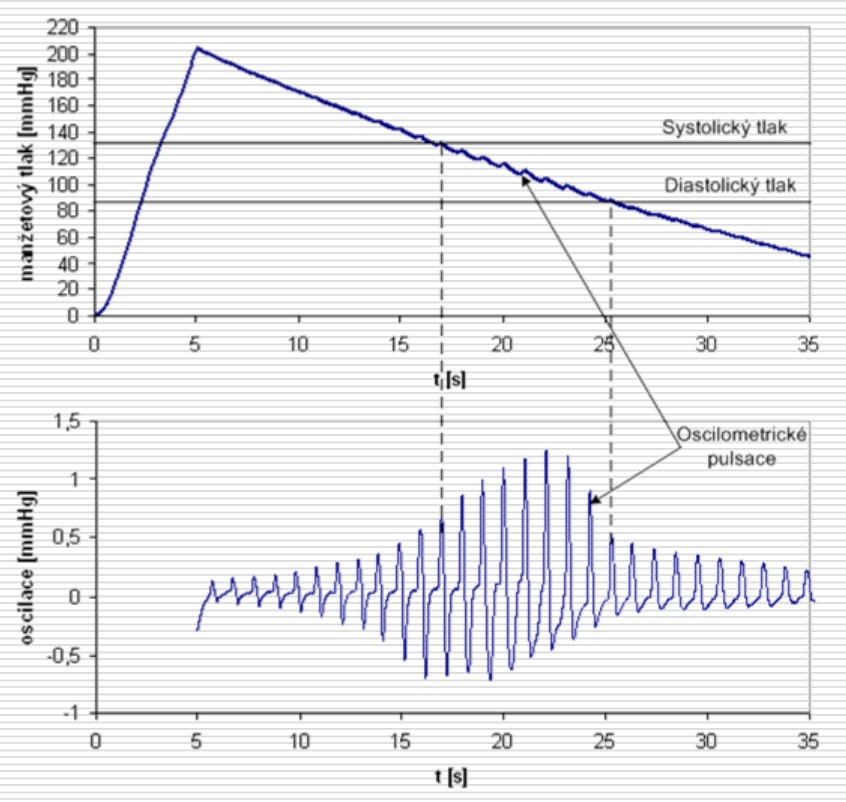
\includegraphics[width=1\textwidth]{pictures/oscilometricky_tlak.jpg}
\end{figure}
\section{Rychlost šíření pulzní vlny}
Rychlost šíření pulzní vlny (PWV) je rychlost, během systolické kontrakce srdce, při které tlaková vlna krve se progpaguje arterieremi. Parametr PWV je jeden ze základních ukazatelů arteriální
elasticity. Čím je hodnota PWV vetší, tím jsou cévy měné poddajné a výsledkem je zvětšená tuhost artérií.
\begin{figure}[H]
    \caption{Postup odražené krevní tlakové vlny v těle}
    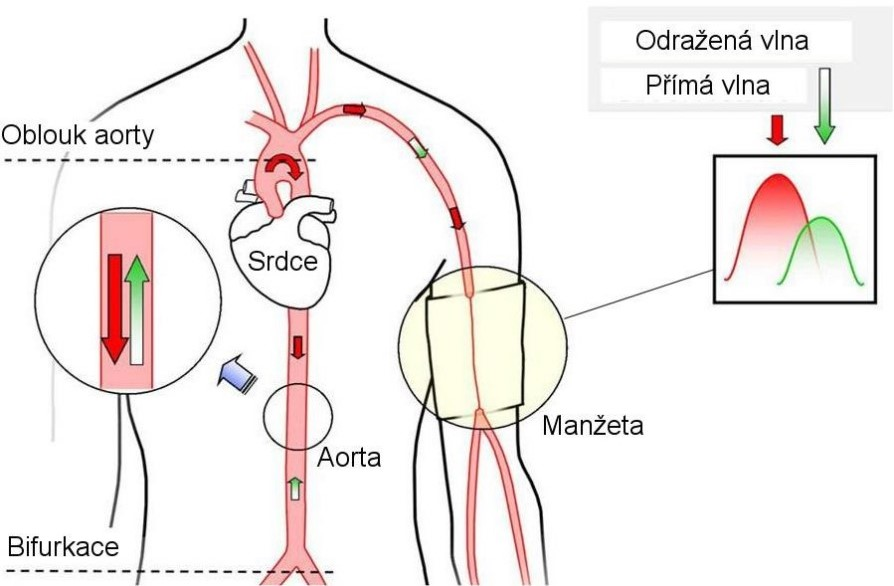
\includegraphics[width=1\textwidth]{pictures/pwv_body.jpg}
\end{figure}
Jeden ze způsobů určení parametru PWV je poměr dvojnásobné vzdálenosti od hrudního zářezu ke stydké kosti $l$ a rozdíl času primární tlakové vlny $t_1$ a odražené tlakové vlny $t_2$.
\begin{equation}
    PWV = \frac{2l}{t_2 - t_1}
\end{equation}
\begin{figure}[H]
    \caption{Krevní tlaková vlna s vyznačenými parametry pro výpočet parametru PWV.}
    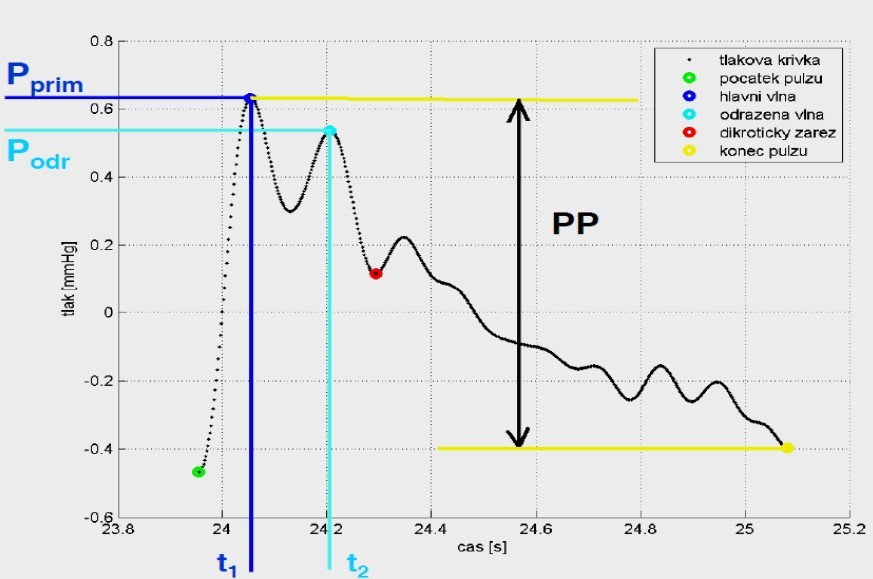
\includegraphics[width=1\textwidth]{pictures/pwv_pressure_wave.jpg}
\end{figure}
\section{Rešerše přístrojů pro měření hemodynamických parametrů krevního řečiště}
Tato sekce se zaměří na validované systémy na trhu pro neivazivní měření hemodynamických parametrů krevního řečiště a to zejména na měření parametru PWV.

\subsection{SphygmoCor XCEL PWA/PWV}
SphygmoCor XCEL PWA/PWV je automatický systém pro analýzu krevní tlakové vlny pomocí pažní manžety.

\begin{figure}[H]
    \caption{SphygmoCor XCEL PWA/PWV}
    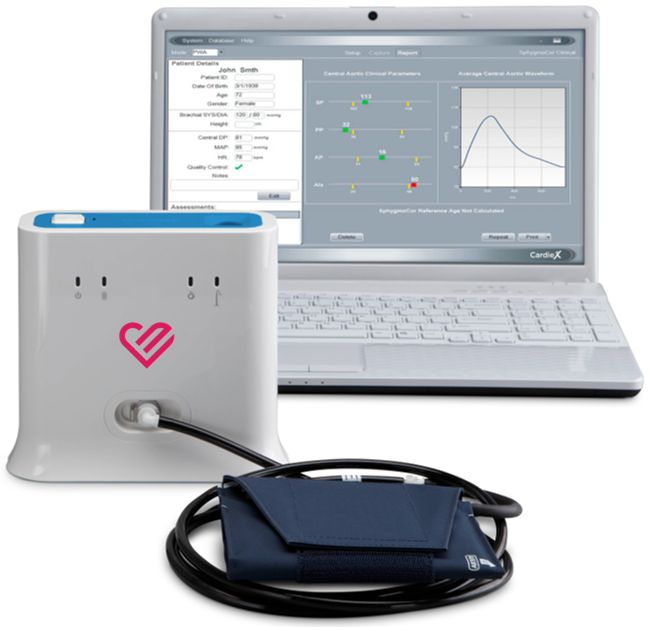
\includegraphics[width=0.5\textwidth]{pictures/XCEL_System.jpg}
\end{figure}
Mezi měřené parametry patří centrální aortální tlak, augmentační index a PWV. Pro měření parametru PWV je potřeba přidaná manžeta na stehno.
\par
Ovládání přístroje je pomocí připojeného osobního počítače přes USB s nainstalovaným softwarem. Software spouští terapii a následně dělá i vyhodnocení naměřených hodnot. Samostatný přístroj není schopný provádět terapii bez osobního počítače a dedikovaného softwaru.
\par
Systém SphygmoCor XCEL je validován pro použití a prodej v Evropské unii a USA. Patří do třídy II.
\subsection{Uscom BP+}
Uscom BP+ je automatizový systém pro měření centrálního krevního tlaku, augmentačního indexu a analýzy křívky krevního tlaku a dalších parametrů.
\begin{figure}[H]
    \caption{Uscom BP+}
    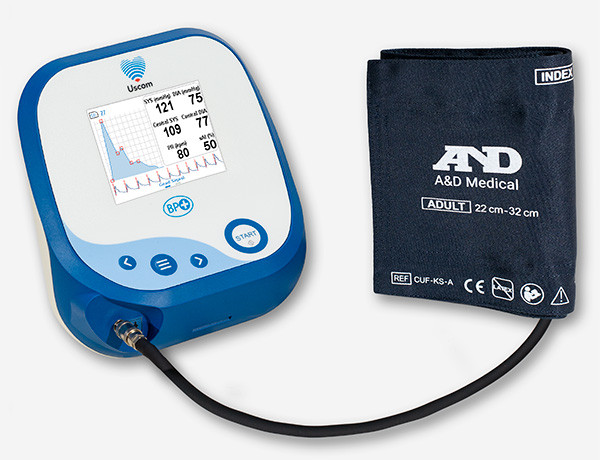
\includegraphics[width=0.6\textwidth]{pictures/uscom_bp.jpg}
\end{figure}
Systém BP+ provádí terapii a analýzu naměřených hodnot v jednom systému tj. bez potřeby nadřazeného systému.

\subsection{Arteriograph}
Arteriograph (Tensiomed) je systém pro neinvazivní měření hemodynamických parametrů krevního řečístě oscilometrickou metodou a pomocí jedné pažní manžety.
Metoda měření oscilometrickou metodou je patentována (US Pat. No. 20070106162) a validována invazivně.
\begin{figure}[H]
    \caption{Tensiomed Arteriograph}
    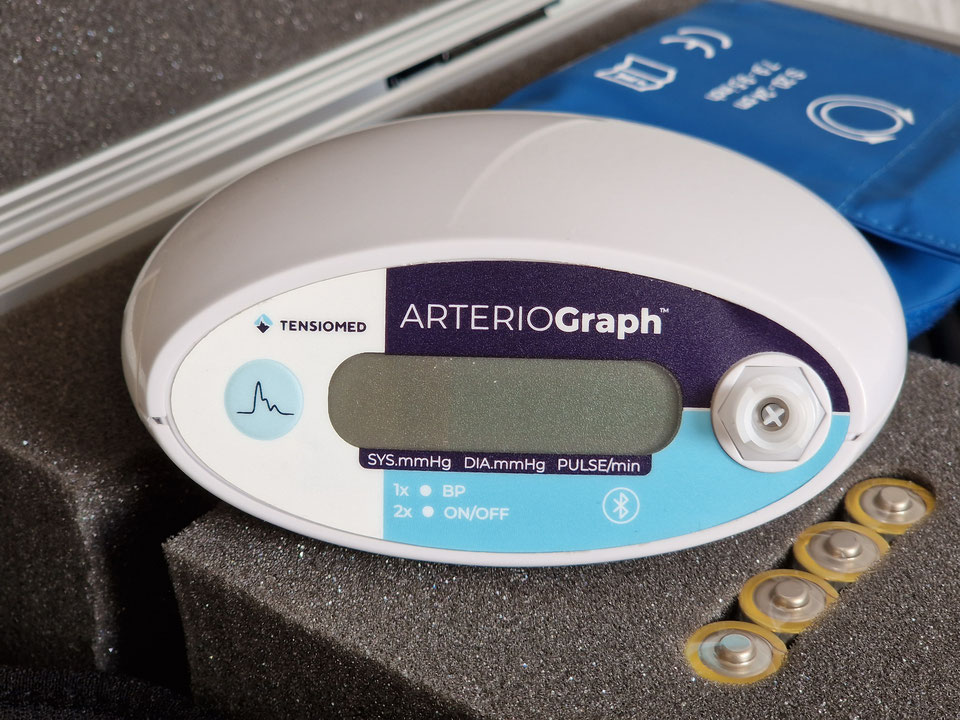
\includegraphics[width=0.6\textwidth]{pictures/arteriograph.jpg}
\end{figure}
Arteriograph může fungovat samostatně pro měření pouze krevního tlaku. Přístup k měření dalších hemodynamických parametrů je potřeba systém připojit k nadřazenému systému pomocí bluetooth s nainstalovaným specializovaným softwarem od Tensiomed.
Po připojení k nadřazenému systému, Arteriograph zasílá během terapie v reálném čase, kde se zpracují naměřené výsledky a zobrází.
%Hardware
%!TEX ROOT=main.tex
\chapter{Hardware}
Zde bude celkovy popis HW vcetne blokovych schemat
zde bude poppis Pouziteho MCU


\section{Řídící jednotka}

Řídící jednotka působí jako centrum řízení a sběru dat. Má na starosti řízení ventilů, natlakování pneumatického systémum, sběr a vyhodnocení
dat ze senzorů a komunikaci s nadřazeným systémem. \par


Jako řídící jednotka byl vybrán mikroprocesor SMT32F407ZG (dále jenom MCU) od firmy ST Microelectronics.
Jádro je Arm® Cortex®-M4 32bit, jehož časovací frekvence může být až $168 \ MHz$. Jádro Cortex-M4 je vhodné pro zpracování signálu díky zabudovanému výpočetnímu modulu Floating Point Unit(FPU) určené na
počítání s desetinými čísly a také řadou instrukcí určené specificky na zpracování signálu.


\begin{figure}[H]
    \centering
    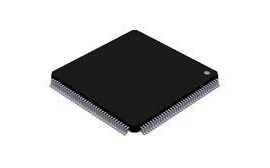
\includegraphics[width=0.5\linewidth]{pictures/stm32f407.jpg}
    \caption{Model stm32f407 \\ \url{https://www.distrelec.cz/cs/mikroradic-32bit-512kb-lqfp-st-stm32f407zet6/p/30170736}}
    \label{fig:stm32}
\end{figure}
MCU je v obalu se 144 piny se 114 vstupně/výstupními piny, 1 MByte FLASH paměti, 256 KByte paměti SRAM, 3x 12 bit AD převodníky s až 24 kanály s maximální vzorkovací frekvencí 2.4 MHz,
2x 12 bit DA převodníky, 14 TIMER, 6x USART, 3x SPI, SysTick Timer a další periferie.
\par
Celkové zapojení MCU je na obrázku \ref{fig:stm32_conection}.

\begin{figure}[H]
    \centering
    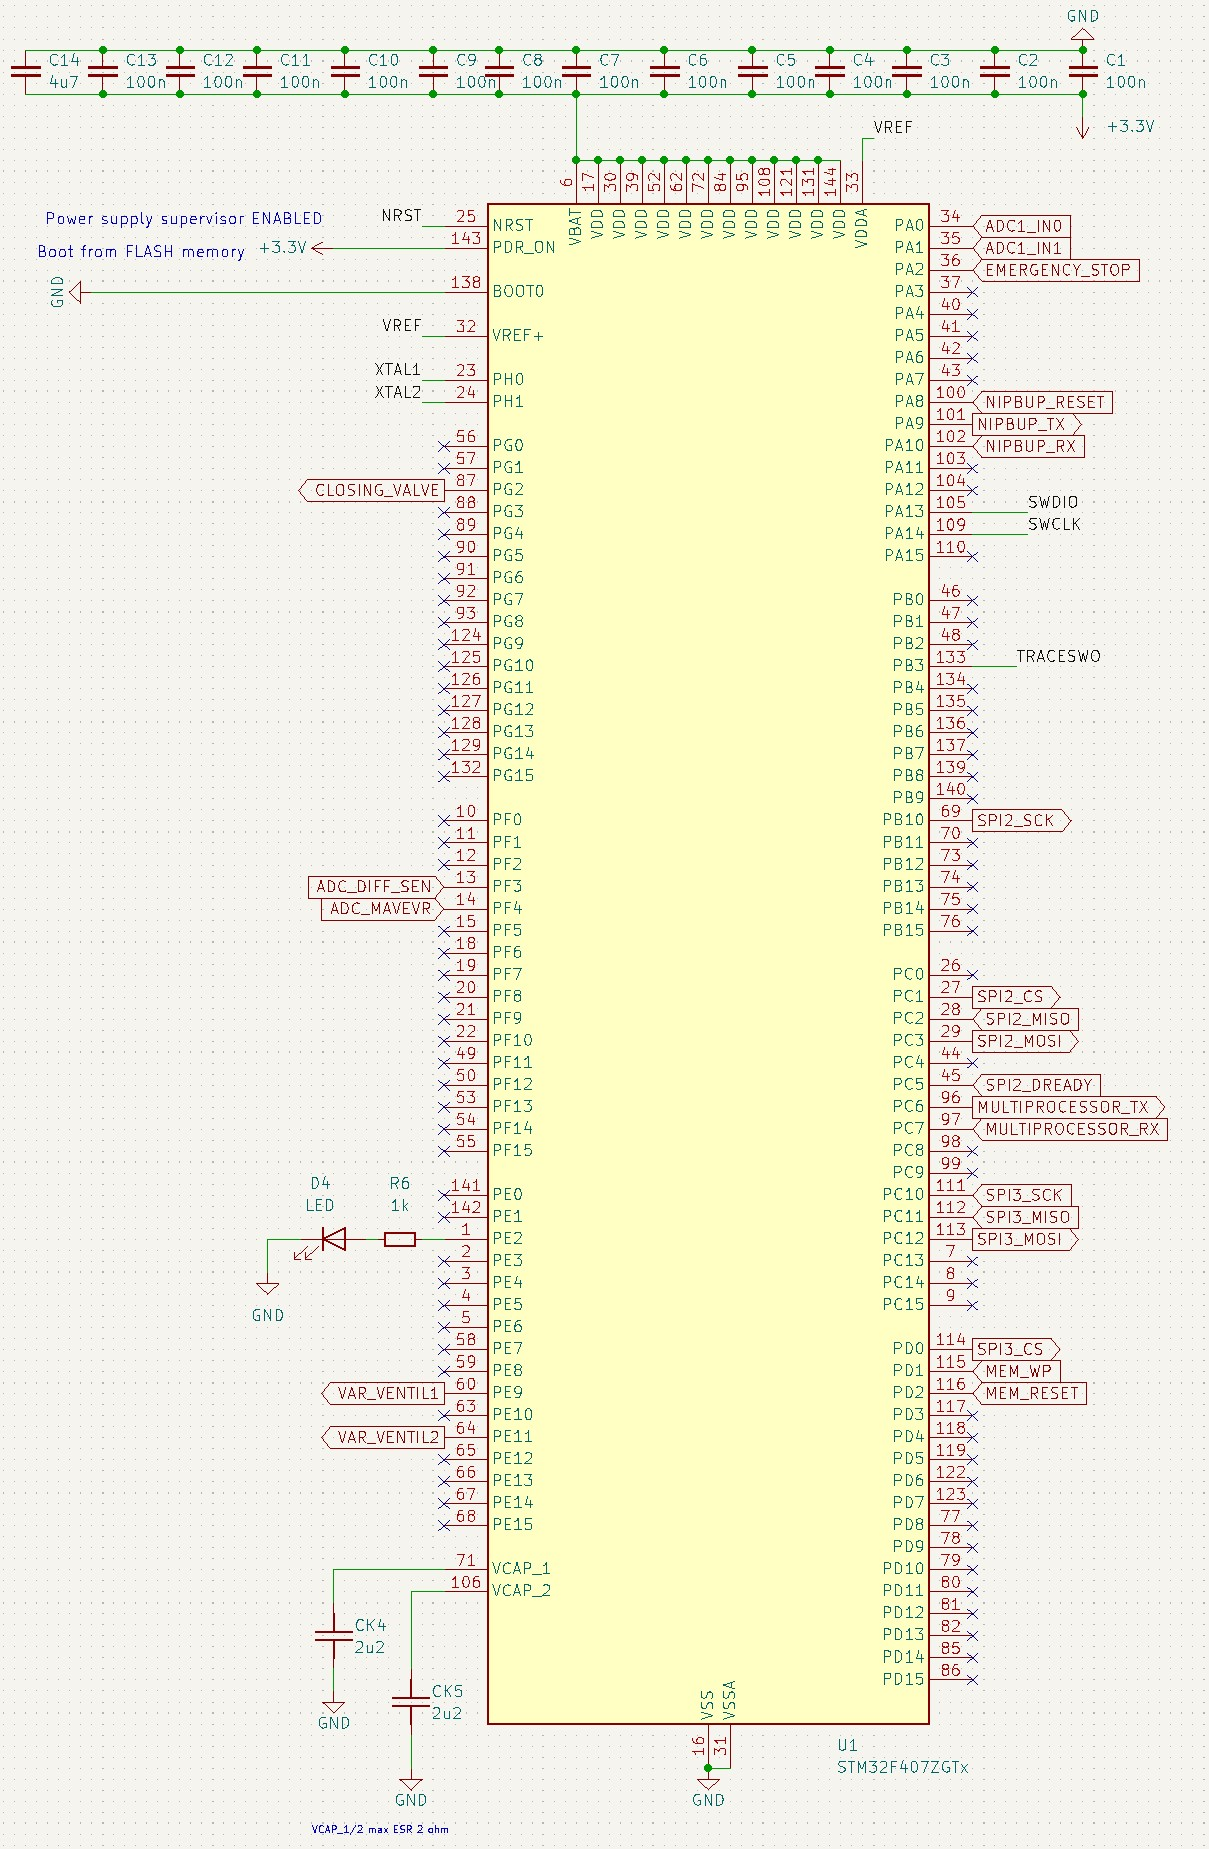
\includegraphics[width=1\linewidth]{pictures/stm_connection.jpg}
    \caption{Schéma zapojení SMT32F407ZG}
    \label{fig:stm32_conection}
\end{figure}

Zapojení MCU je podle doporučeného zapojení. Jedná se hlavně o umístění a typy blokovacích kondenzátorů, reset signál, boot z interní nebo externí flash paměti a zvolení externích nízko a vysoko kmitočtových hodin. \par

\subsection{Externí hodiny}

MCU obsahuje interní vysokorychlostní RC oscilátor, ale pro maximální přesnost a spolehlivost byl zvolen externí vysokorychlotní oscilátor Abracon ABM3 o frekvenci  $8 \ MHz$. Externí oscilátor slouží jako hlavní časovací hodiny pro
jádro. Jádro může být na frekvenci až $168 \ MHz$ a to pomocí vnitřní násobičky frekvence Phase Locked Loop (dále pouze PLL) můžeme dosánout z $8 \ MHz$.

\begin{figure}[H]
    \centering
    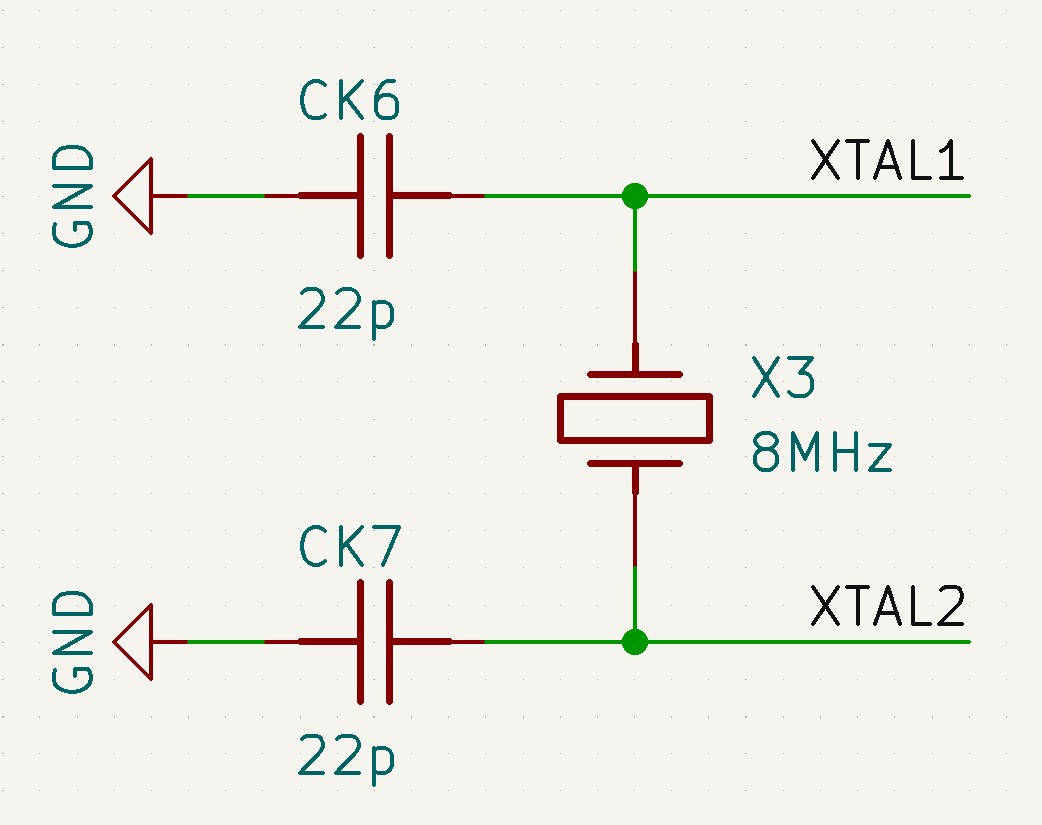
\includegraphics[width=0.8\linewidth]{pictures/stm32_hse.jpg}
    \caption{Schéma zapojení vysokorychlostního externího oscilátoru pro STM32}
    \label{fig:stm32_hse}
\end{figure}

Snížení frekvence externích hodin omezíme vysoko frekvečního rušení, případného přeslechu na vodičích a celkové signálové integritě.


\subsection{Napěťová reference pro analogové periferie} \label{section:vref}
Pro dosáhnutí nejpřesnějšího měření, je třeba, aby analogová čast byla co nejméně zarušena. Díky vysokým kmitočtům digitální čast MCU může zarušit analogové periférie a proto jsou v MCU digitální a analogové obvody oddělené.
Jako refereční napětí je použito zapojení na obrázku \ref{fig:stm32_vref}.

\begin{figure}[H]
    \centering
    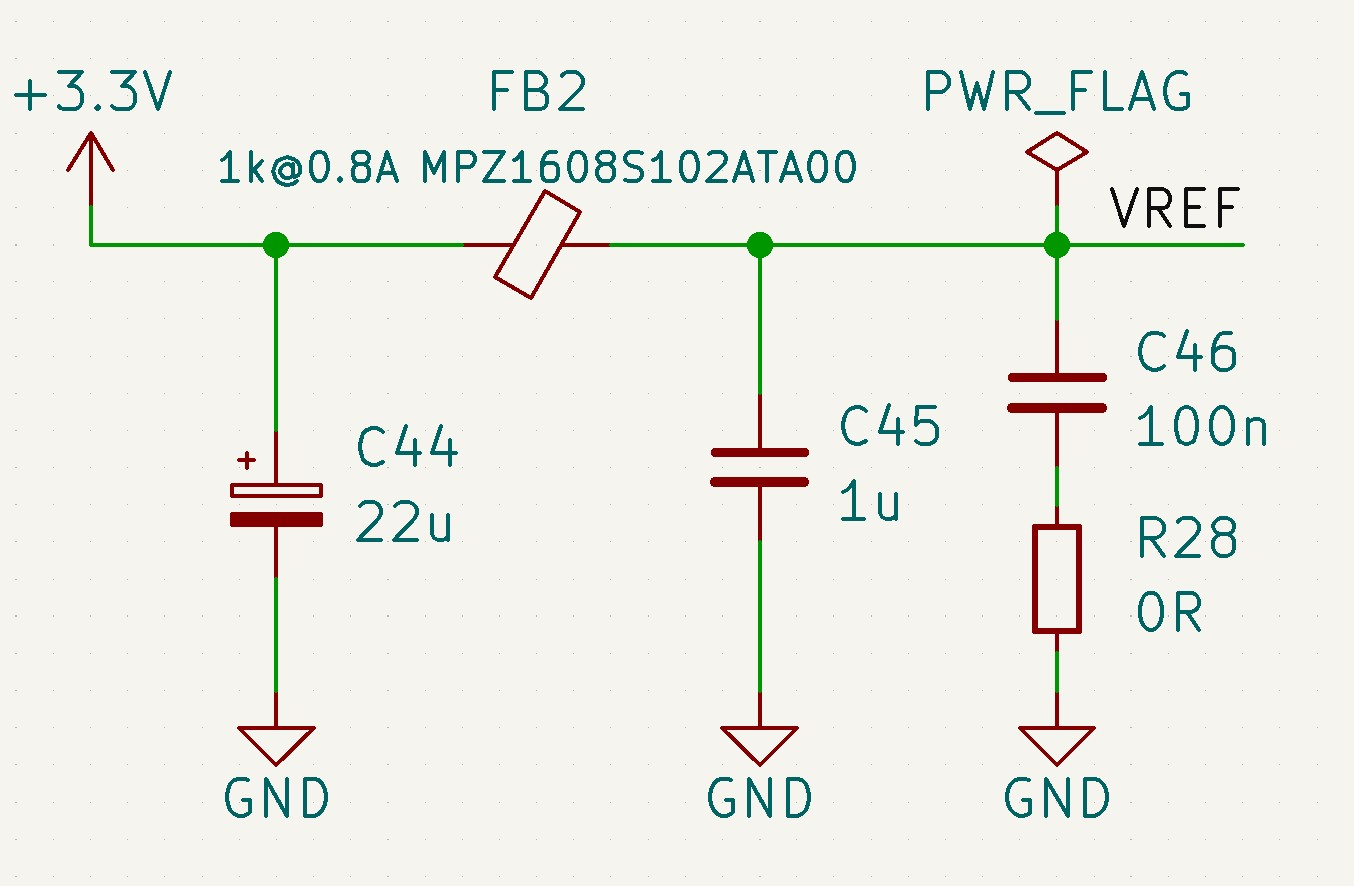
\includegraphics[width=1\linewidth]{pictures/stm_analog_reference.jpg}
    \caption{Schéma zapojení referečního napětí pro analogové periférie STM32}
    \label{fig:stm32_vref}
\end{figure}

Tento filtr začne potlačovat na frekvenci $f = 138 \ kHz$. Ale mezi $\approx 50 \ kHz$ a $ \approx 115 \ kHz$ filtr zesiluje, kde největší zesílení o $19 \ dB$ je na frekvenci $88.8 \ kHz$

\begin{figure}[H]
    \centering
    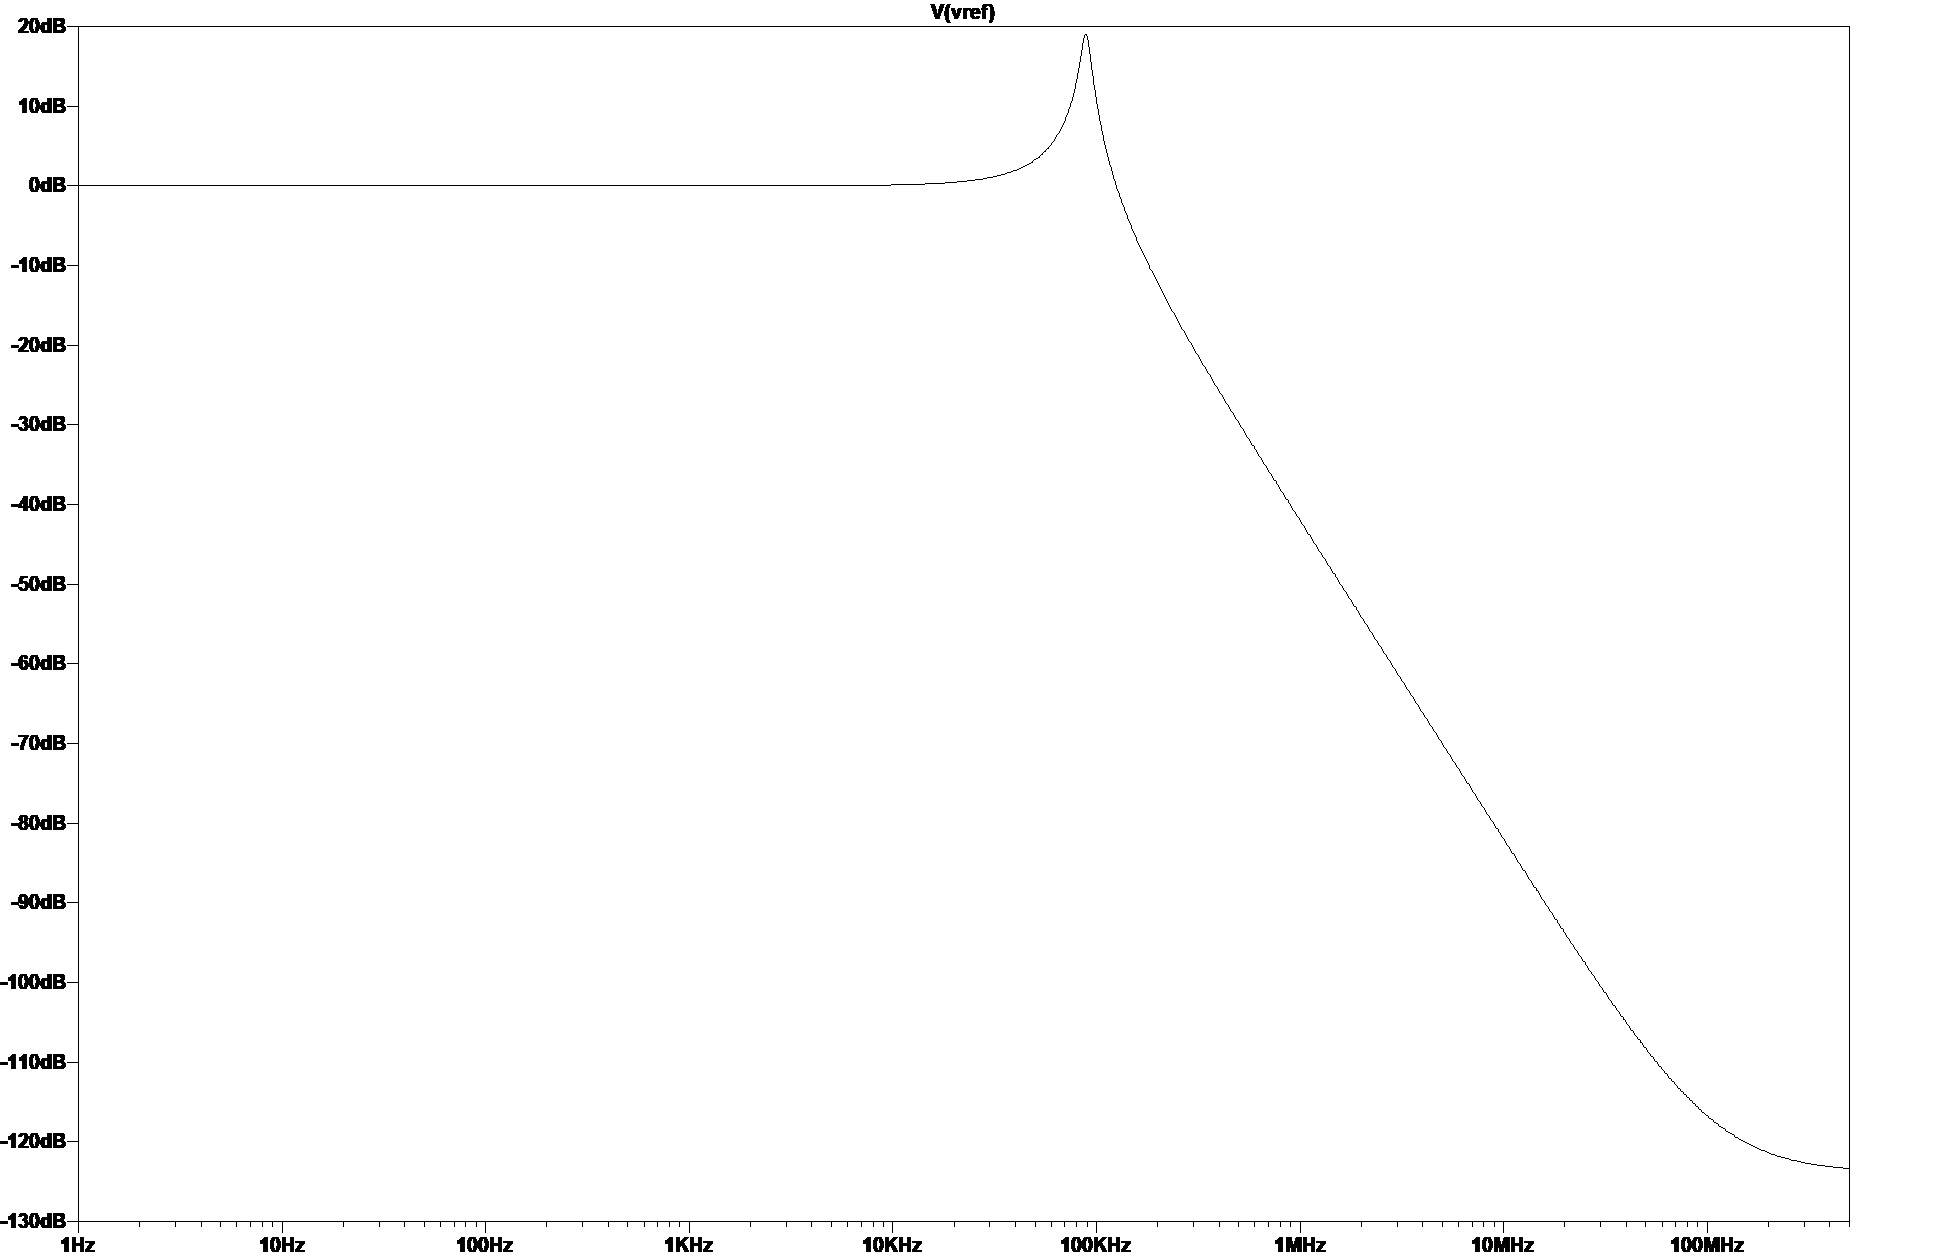
\includegraphics[width=1\linewidth]{pictures/cardi_vref_filter_response.jpg}
    \caption{Aproximace frekveční odezvy filtru analogového napětí.}
    \label{fig:stm32_vref_response}
\end{figure}

Feritový korálek je pasivní součástka, který se používá pro filtraci vysokofrekvenčního rušení přes širokou část frekvenčního rozsahu. Největší impedanci má okolo určené frekvence a disipuje energii rušení ve formě tepla.
\subsection{Ochrana proti elektrostatickému výboji}
Elektrostatický výboj(ESD) je náhlý a krátkodobý elektrický proud mezi dvěma objeky s různým elektrickým potenciálem. Představuje horzbu elektrickým komponentům ve formě trvalého, nevratného poškození. Nejčastější místa probití jsou zejména místa, kterých se často dotýkáme například kontektory.
\par
Jako ochrana je použita transient voltage suppression (TVS) dioda D5V0F1U2S9-7 od firmy Diodes Incorporated.

\begin{figure}[H]
    \centering
    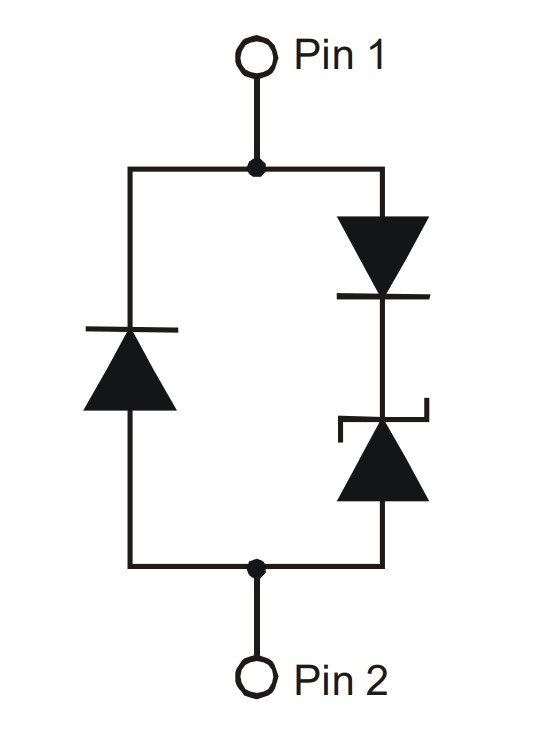
\includegraphics[width=0.4\linewidth]{pictures/esd_diode_schema.jpg}
    \caption{Schéma ochrané ESD diody D5V0F1U2S9-7. Kde Pin 1 je katoda.}
    \label{fig:esd_diode}
\end{figure}

Tato dioda je určená pro ochranu proti elektrostatickým výbojům. Je připojena v závěrném směru na všechny konketory. V závěrném směru bude otevřena při napětí
$U = 5.5 \ V $ a napětí omezí na $U_{BR} = 6.0 \ V $.

\section{Modul měření krevního tlaku}

Součástí pneumatické části je modul PAR Medizintechnik NIBP 2020 UP , který omužňuje validované měření krevního tlaku oscilometrickou metodou v průběhu nafukování, také vyfukování, a následné nafouknutí na suprasystolický tlak. Samotné nafukování pneumatického systému je realizováno z elektromechanické vzduchové pumpy integrované v modulul PAR.
Pneumatická část modulu PAR se skládá ze vzduchové pumpy se zpětným ventilem zamezujícím úniku tlaku, vypouštějícího ventilu, tlakového senzoru a také redundantním sensorem tlaku a vypouštěcím ventilem pro případ poruchy. \par
Modul PAR má klinickou validaci pro měření krevního tlaku dle norem DIN EN 80601-2-30, DIN EN 81060-2 a systém podle norem DIN EN 60601-1 (2. a 3. edice), DIN EN 60601-1-2, DIN EN 60601-1-6.
\begin{figure}[H]
    \centering
    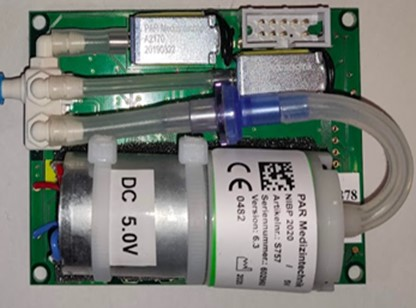
\includegraphics{pictures/par_nibp_up.jpg}
    \caption{Tlakový modul PAR NIBP 2020 UP}
    \label{fig:par_modul}
\end{figure}

Pneumatická část je řízena procesorem, se kterým lze komunikovat pomocí datové sériové linky RS232 či TTL a standardního protokolu CAS s rychlostí 4800 baud. Do modulu jsou posílány přes rozhraní UART příkazy pro nastavení režimu a parametrů zakončené příkazem pro zahájení měření.
\begin{figure}[H]
    \centering
    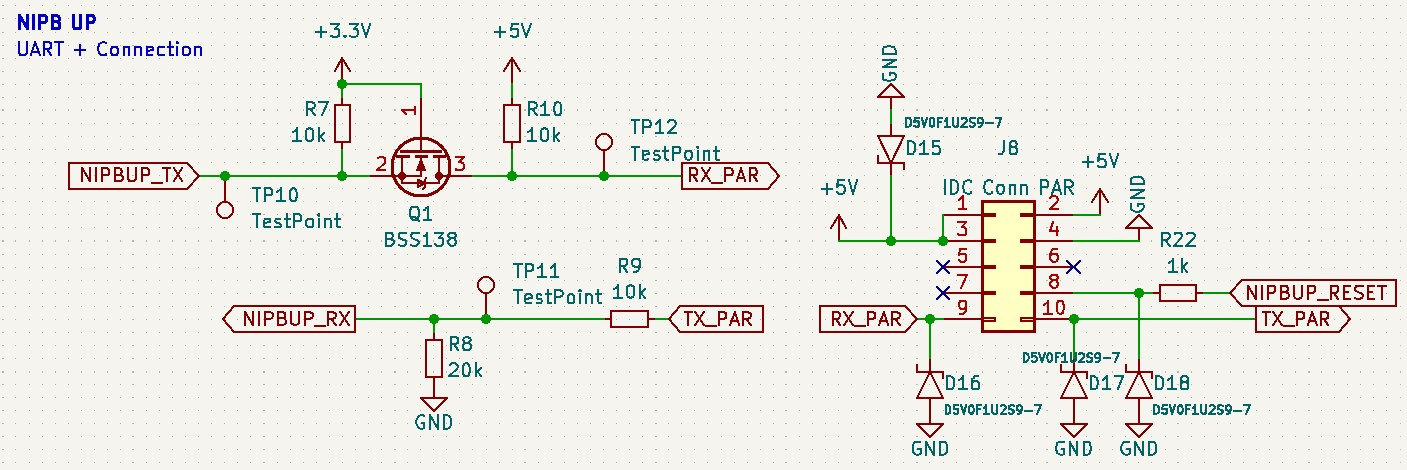
\includegraphics[width=0.9\linewidth]{pictures/nibpup_connection.jpg}
    \caption{Schéma připojení komunikační linky k MCU a napájení pro PAR NIBP 2020 UP }
    \label{fig:par_modul_comm}
\end{figure}
Pneumatickou část lze udržovat na hladinách tlaku v rozmezí (0–300) mmHg po dobu až 180 s a uživateli umožňuje zvolit odstup suprasystolického tlaku od naměřeného systolického tlaku. Po odeslání příkazu pro zahájení měření posílá modul po lince aktuální stav pneumatické části během celého měření a po měření posílá zprávu s naměřenými hodnotami krevního tlaku a srdeční frekvence.
\section{Senzory}
Tato sekce se zaměří na popis a použití senzorů a to zejména tlakových. Tlakové senzory tvoří nezbytnou část celkového přistroje a rozhodují o celkovém konfortu pacienta a také o přesnost výsledné terapie. \par
Parametry senzorů tlaku vychází z parametrů terapie. Pneumatický systém může být pod tlakem až $300 \ mmHg = 40 \ kPa$, tento požadavek musí splňovat všechny senzory napojené do pneumatického systému.

\subsection{Senzor tlaku} \label{section:pressure_sen}
Senzor tlaku se používá na snímání tlaku v jednotlivých větvý pneumatického systému. \par


Použité sensory tlaku jsou NPX MP3V5050GC6U.

\begin{figure}[H]
    \centering
    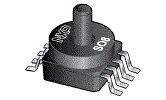
\includegraphics[width=0.5\linewidth]{pictures/nxp_sensor.jpg}
    \caption{Senzor tlaku NPX MP3V5050GC6U}
    \label{fig:nxp}
\end{figure}

Je to analogový sensor tlaku od firmy NXP ze série peizorezistivních převodníků. Parametry jsou následovné:
\begin{table}[H]
    \label{tab:nxp_properties}
    \caption{Properties of nxp sensor}
    \begin{ctucolortab}
        \begin{tabular}{ccccccc}
            \toprule
            Charakteristika                                         & Symbol        & Min & Typ   & Max        & Jednotka         & \\ \midrule
            Rozsah tlaku                                            & $P$           & 0   & -     & 50         & $kPa$            & \\
            Vstupní napětí                                          & $U_{s}$       & -   & 3.3   & -          & $V$              & \\
            Vstupní proud                                           & $I_{s}$       & -   & 10    & -          & $mA$             & \\
            Napěťový offset($0^{\circ}$ až $ 85^{\circ}  C $)       & $U_{off}$     & -   & 0.188 & -          & $V$              & \\
            $\textnormal{Full Scale Output}^{(\ref{enum:nxp_fso})}$ & $U_{FSO}$     &     & 2.77  &            & $V$              & \\
            Přesnost($0^{\circ}$ až $ 85^{\circ} C$)                & -             & -   & -     & $\pm 2.5 $ & $\%$             & \\
            Citlivost                                               & $\frac{U}{P}$ & -   & 54    & -          & $\frac{mV}{kPa}$ & \\
            \bottomrule
        \end{tabular}
    \end{ctucolortab}

    \begin{enumerate}
        \item \label{enum:nxp_fso} Maximální napětí při největším hodnoceném tlaku.
    \end{enumerate}
\end{table}

Zapojení senzoru je na separátní DPS podle doporučeného schématu \ref{fig:nxp_recommended} z datasheetu.
\begin{figure}[H]
    \centering
    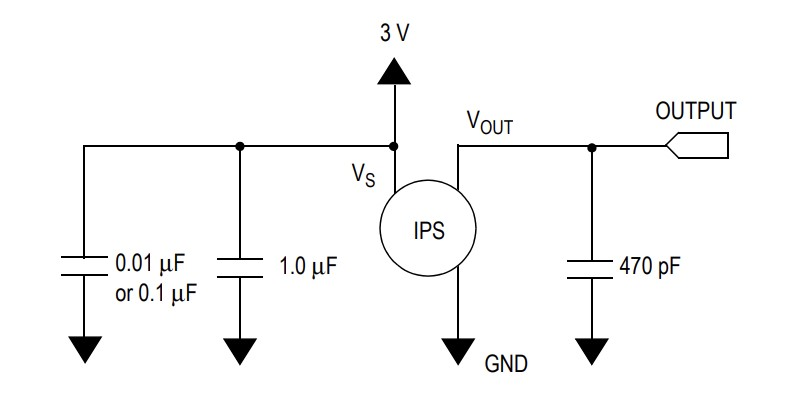
\includegraphics[width=0.9\linewidth]{pictures/nxp_recommended.jpg}
    \caption{Doporučené schéma zapojení senzoru tlaku NPX MP3V5050GC6U. Kde $V_S$ je vstupní napájecí napětí a $V_{out}$ je výstupní napětí.}
    \label{fig:nxp_recommended}
\end{figure}
Analogový výstup ze sensoru je připojen na interní AD převodník MCU.
\subsubsection{Převodní charakteristika}
Převodní charakteristika výstupního napětí $U_{o} \ V$ na tlak $P \ kPa$je
\begin{equation}
    P = \frac{U_o \pm ERROR}{0.018 \cdot U_s} - \frac{0.04}{0.018}
    \label{eq:nxp_transfer}
\end{equation}

\begin{figure}[H]
    \centering
    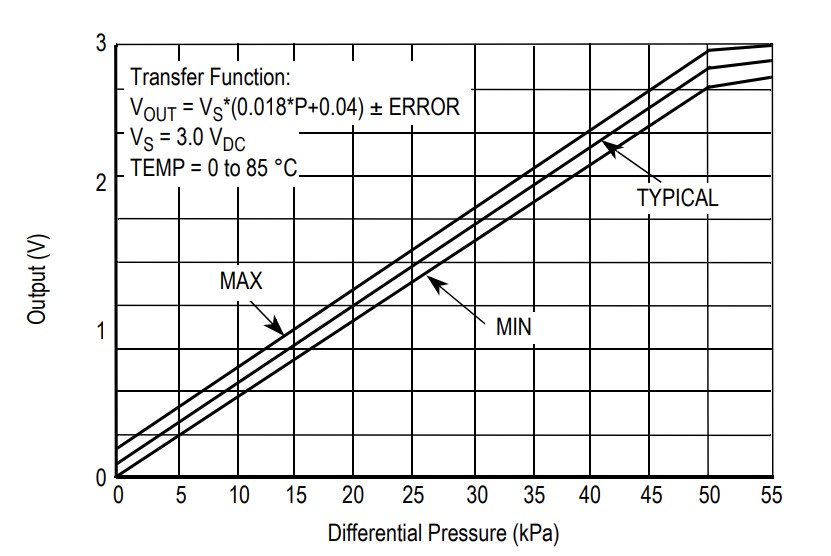
\includegraphics[width=0.9\linewidth]{pictures/nxp_transfer.jpg}
    \caption{}
    \label{fig:nxp_transfer}
\end{figure}

\subsection{Diferenční sensor tlaku} \label{section:diff_pressure_sen}
Diferenční sensor tlaku slouží na snímání malých tlakových pulzací. Porovnává tlak mezí první a druhou (referenční) větvý systému. Po natlakování pneumatického systému až na $300 \ mmHg$ uzavírací ventil oddělí systém na dvě větve. Rozdíl tlaků ve větvy může být $300 \ mmHg$ neboli $40 \ kPa$. \par
Diferenční sensor tlaku byl zvolen Amphenol ELVH-L02D-HRRD-C-NAA4. Je to analogový senzor tlaku určený na snímání ultra nízkých tlaků.
\begin{figure}[H]
    \centering
    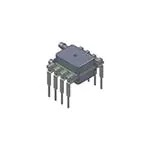
\includegraphics[width=0.3\linewidth]{pictures/amphenol.jpg}
    \caption{Diferenční sensor tlaku Amphenol ELVH-L02D-HRRD-C-NAA4}
    \label{fig:amphenol}
\end{figure}


\begin{table}[H]
    \label{tab:amphenol_properies}
    \caption{properties of an amphenol}
    \centering
    \begin{ctucolortab}
        \begin{tabular}{ccccccc}
            \toprule
            Charakteristika                                                         & Symbol    & Min     & Typ        & Max         & Jednotka & \\ \midrule
            Rozsah tlaku                                                            & $P$       & -497.68 & -          & 497.68      & $Pa$     & \\
            $\textnormal{Proof pressure}^{(\ref{enum:amp_proof_pressure})}$         & $P_{pp}$  & -       & 67         & -           & $kPa$    & \\
            $\textnormal{Průrazný tlak}^{(\ref{enum:amp_burst_pressure}) }$         & $P_{bp}$  & -       & 103        & -           & $kPa$    & \\
            $\textnormal{Common mode pressure}^{(\ref{enum:amp_common_pressure})} $ & $P_{cm}$  & -       & 103        & -           & $kPa$    & \\
            Vstupní napětí                                                          & $U_{s}$   & -       & 3.3        & -           & $V$      & \\
            Vstupní proud                                                           & $I_{s}$   & -       & 2.1        & 2.8         & $mA$     & \\
            Napěťový offset                                                         & $U_{off}$ & -       & 1.65       & -           & $V$      & \\
            $\textnormal{Full Scale Span}^{(\ref{enum:amp_fss})} $                  & $U_{FSS}$ &         & $\pm 1.32$ &             & $V$      & \\
            Přesnost                                                                & -         & -       & -          & $\pm 0.25 $ & $\%$     & \\
            Citlivost                                                               & -         & -       & 0.2        & -           & $\%$     & \\
            \bottomrule
        \end{tabular}
    \end{ctucolortab}
    \begin{enumerate}
        \item \label{enum:amp_proof_pressure} Maximální tlak, který může být aplikován na jeden z portů senzoru a zachoval původní specifickace.
        \item \label{enum:amp_burst_pressure} Maximální tlak, který může být aplikován na jeden z portů senzoru, bez způsobení úniku tlaku.
        \item \label{enum:amp_common_pressure} Maximální tlak, který může být aplikován na oba porty zároveň, bez způsobení úniku tlaku.
        \item \label{enum:amp_fss} Algebraický rozdíl napětí při nejmenším možném specifikovaném tlaku a při maximálním specifikovaném tlaku.
    \end{enumerate}
\end{table}
\raggedbottom
Analogový signál ze senzoru je připojen k 24 bit AD převodníku přes RC článek. Schéma zapojení k AD převodníu je \ref{fig:amphenol_circuit}

\begin{figure}[H]
    \centering
    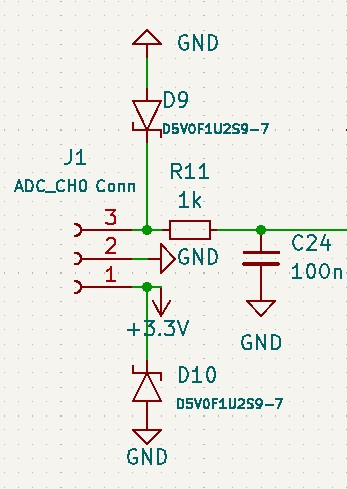
\includegraphics[width=0.7\linewidth]{pictures/diff_sen_circuit.jpg}
    \caption{Schéma zapojení diferenčního sensoru tlaku Amphenol ELVH-L02D-HRRD-C-NAA4 k AD převodníku.}
    \label{fig:amphenol_circuit}
\end{figure}

\raggedbottom
Zlomová frekvence RC článku $f_0 = \frac{1}{2 \pi RC} = 1591 \ Hz $ byla spočítána podle maximální frekvence tlakové vlny.

\begin{figure}[H]
    \centering
    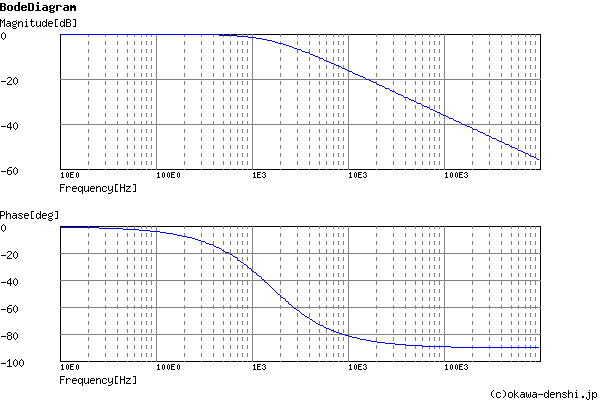
\includegraphics[width=0.9\linewidth]{pictures/rc_1k_100n_1591.png}
    \caption{Bodeho aproximace RC článku pro Amphenol ELVH-L02D-HRRD-C-NAA4}
    \label{fig:amphenol_filter}
\end{figure}

Podle Bodeho fázové aproximace RC článku na obrázku \ref{fig:amphenol_filter} můžeme vidět, že fáze se začne měnit před $\frac{f_0}{10}$.
Změna fáze snímaného signálu způsobí zkreslení výsledných hodnot a nepřesnou terapii.
\section{Vzduchové ventily}
Ventily jsou důležitou součástí pneumatického systému. Starají se o správný průběh terapie a také o bezpečí pacienta. \par
V systému rozlišujeme dva druhy vzduchových ventilů, uzavírací a vypouštějcí regulační. Uzavíraci ventil slouží pro oddělení manžety a pumpy. Vypouštěcí regulační ventily jsou na obou větvých pneumatického systému. Slouží jako pro regulaci tlaku v systému během terapie a také jako nouzové vypouštěcí ventily. \par
Všechny použité ventily nesmí v uzavřeném stavu propustit vzduch při tlaku $300 \ mmHg$, jinak by hrozilo nepřesné výsledky při měření a tím pádem špatná terapie.

\subsection{Uzavírací ventil}
Uzavírací ventil je důležitou součástí systému. Pneumatický systém rozdělí na dvě větve, kde jedna je část s manžetou a druhá větěv je jako referenční. \par

\begin{figure}[H]
    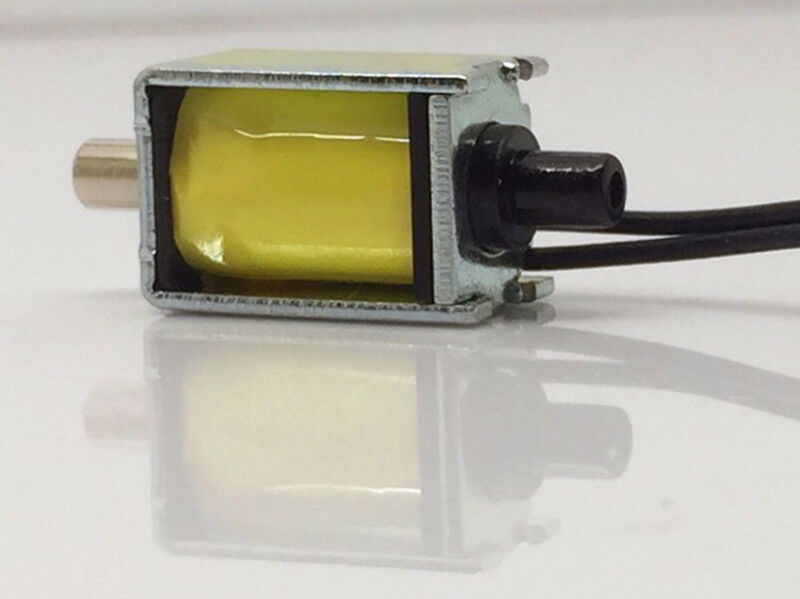
\includegraphics[width=0.9\linewidth]{pictures/closing_valve.jpg}
    \caption{Fotka uzavíracího ventilu CJAV08-2B05A1}
    \label{fig:closing_valve}
\end{figure}

Pro tento účel je použit ventil CONJOIN CJAV08-2B05A1. Je to řízený napětím, normálně zavřený, vzduchový ventil typu solenoid  o $U = 5 \ V$ a vstupní proud o $I = 204 \ mA \pm 10\% $

\begin{figure}[H]
    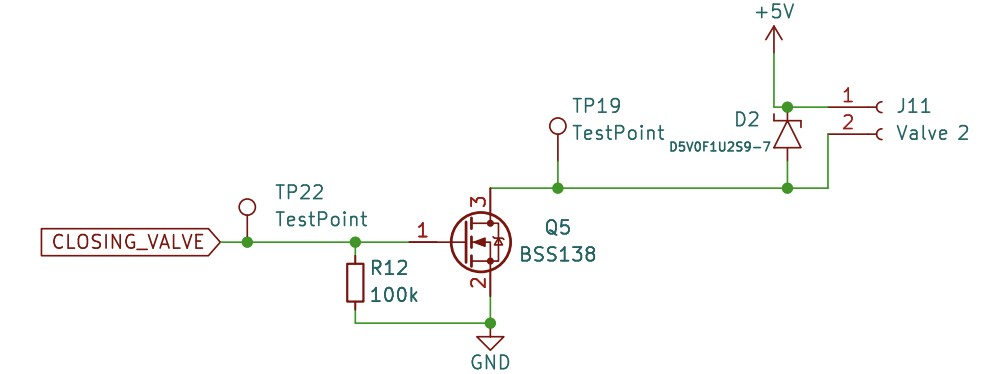
\includegraphics[width=0.9\linewidth]{pictures/closing_valve_driver.jpg}
    \caption{Schéma zapojení uzavíracího ventilu}
    \label{fig:closing_valve_driver}
\end{figure}

Pro řízení ventilu z výstupního pinu MCU je použitý NMOS tranzistor BSS138. BSS138 má spínací práh napětí $U_{GS} = 3.3 \ V$ což je přímo výstupní napětí z GPIO a maximální proud přes drain je $I_D = 0.22 \ A$. Resistor přes Gate a Source zajisti známé napětí, pokud bude vstup na Gate plovoucí. Tím se zamezí neznámé chovaní tranzistoru.

\subsection{Regulační ventil}
Regulační ventily slouží k regulaci tlaku v systému při terapii a také jako vypouštěcí ventily pro vrácení pneumatického systému na atmosférický tlak. Ventily jsou umístěné na každe větvy pneumatického systému. Během terapie je možno si zvolit jak moc vysoký průtok vzduchu je možný, tím můžeme regulovat tlak v obou větvých podle potřeby terapie. \par

Regulační ventily jsou použité JQF4-6A/DC6V. Je to normálně otevřený lineární solenoid ventil. Maximální povolený tlak je $350mmHg$, řízený napětím $U = 6 \ V$ DC a proudový odběr je $I = 0.107 \ A$.\par

Napětí na ventilech je $5V$ i přes to, že ventily požadují napětí $6 \ V$. Sadou testů zjístilo, že momentální napětí vyhovuje naším požadavkům a únik tlaku při plném sevření nijak neovlivňuje terapii a přidáním $6 \ V$ by se akorát zvýšila komplexita systému.

\begin{figure}[H]
    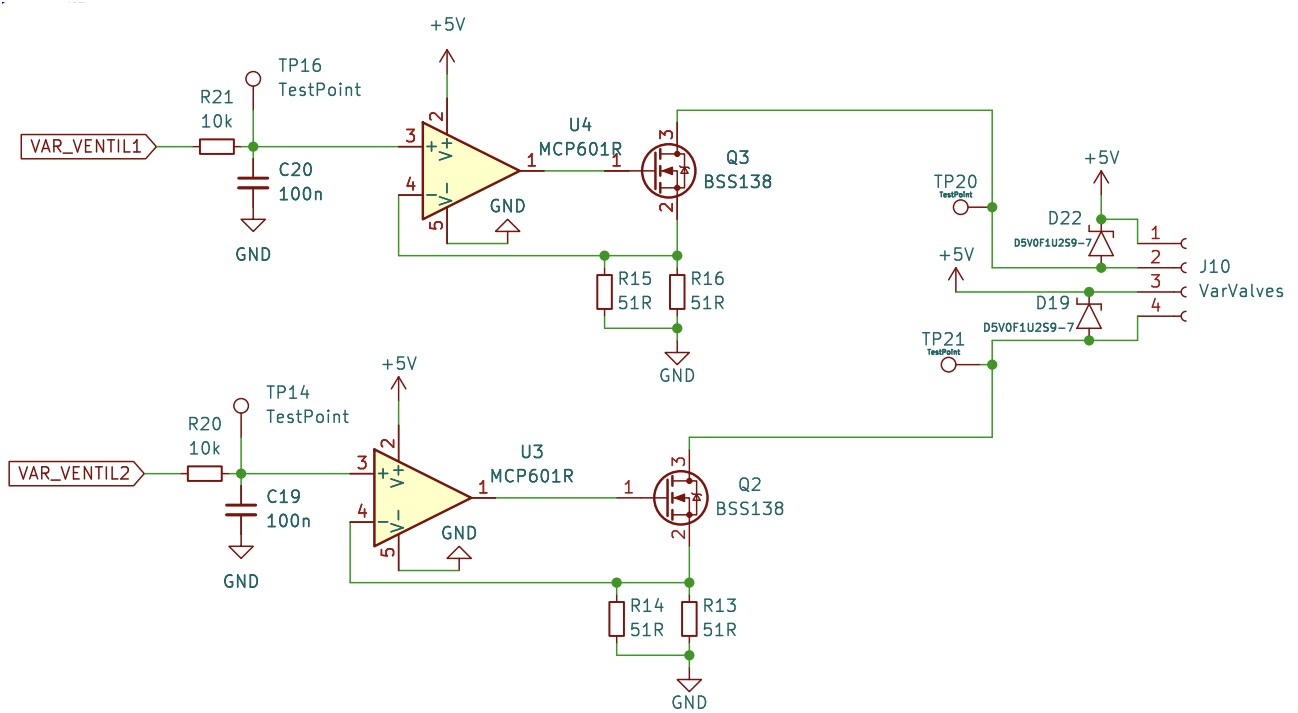
\includegraphics[width=1\linewidth]{pictures/var_valves.jpg}
    \caption{Schéma zapojení regulačních ventilů}
    \label{fig:variable_valve_driver}
\end{figure}

\subsubsection{Zdroj proudu}
Regulační ventily jsou řízené napěťově řízeným zdrojem proudu jak je na obrázku \ref{fig:variable_valve_driver}.\par
Ventily jsou napojené na drain NMOS tranzistoru, přes který jde konstatní napětí požadované ventilem. Proud se řídí operačním zesilovačem, který má na neinvertujícím vstupu $U_+$ napojené řídící napětí $U_i$. Výstup operačního zesilovače je spojen s gate tranzistoru. Source tranzistoru je spojen s invertujícím vstupem $U_-$ operačního zesilovače a také paralelně k zemi jsou zapojené resistory $R_{||}$, které určují maximální možný proud na regulačních ventilech. Výsledný proud je:
\begin{equation}
    \label{eq:current_source}
    I = \frac{U_i}{R_{||}}
\end{equation}
V případě na obrázku \ref{fig:variable_valve_driver} paralelní resistory $R_1 = R_2 = 51 \ \Omega$ mají výslednou hodnotu:
\begin{align*}
    R_{||} = \frac{R_1 R_2}{R_1 + R_2} = \frac{51}{2} = 25.5 \ \Omega
\end{align*}
Maximálním napětí, které umožní MCU z GPIO pinu je $3.3V$ proto maximální možný proud na regulačních ventilech je:
\begin{align*}
    I = \frac{U_i}{R_{||}} = \frac{3.3}{25.5} \approx 129 \ mA
\end{align*}

Pokud budeme brát v úvahu ideální OZ, tak do invertujícího $U_-$ a neinvertujícího $U_+$ vstupu jde nulový proud, kde $U_+ = U_-$ a výstup z OZ je
\begin{align}
    U_o = A(U_+ - U_-)
\end{align}
kde $A [-] $ je zesilovační činitel, který se blíží k nekonečnu. Pokud bude na výstupu OZ nulové napětí, tranzistor je uzavřen a napětí na source je také nulové. Pokud ale například dáme řídící napětí třeba na $U_i = 1V$, poté se OZ bude snažit, aby rozdíl $U_+ - U_- = 0$, tak na výstupu OZ se bude zvyšovat napětí dokud napětí na source nebude $U_- = U_i$. To znamená, že přes regulační ventily právě bude procházet proud z rovnice \ref{eq:current_source}.

Použitý NMOS tranzistor je BSS138, který má minimální práhové napětí $U_{GS(th)} = 0.5 \ V$, to je napětí, při kterém začne protékat proud. To znamená, že minimální řídící napětí musí být $U_{i} = 0.5 \ V$


\subsubsection{Řídící signál}
Řídící signál je čtvercový pro řízení proudového zdroje. PWM signál z MCU o frekvenci $f_{PWM} = 25 kHz$ je filtrován pomocí RC článku o zlomové frekvenci $f_c = 159 Hz$, který slouží pro modulaci řídícího PWM signálu na konstatní napětí.
\par
Pulse Width Modulated(PWM) signál je periodický čtvercový signál s fixní periodou a měnící se poměrem času v log.1 a log.0, také nazývané jako střída(Duty Cycle). Průměrné napětí PWM signálu je
\begin{equation}
    U_{out} = U_{max} \cdot Duty Cycle
\end{equation}
kde $U_{max}$ je maximální amplituda PWM signálu. \par


Pomocí fourierovy analýzy PWM signálu můžeme vidět, že PWM signál se neskládá pouze z jedné frekvence, ale z mnoha (Obrázek \ref{fig:pwm_spectrum}).

\begin{figure}[H]
    \centering
    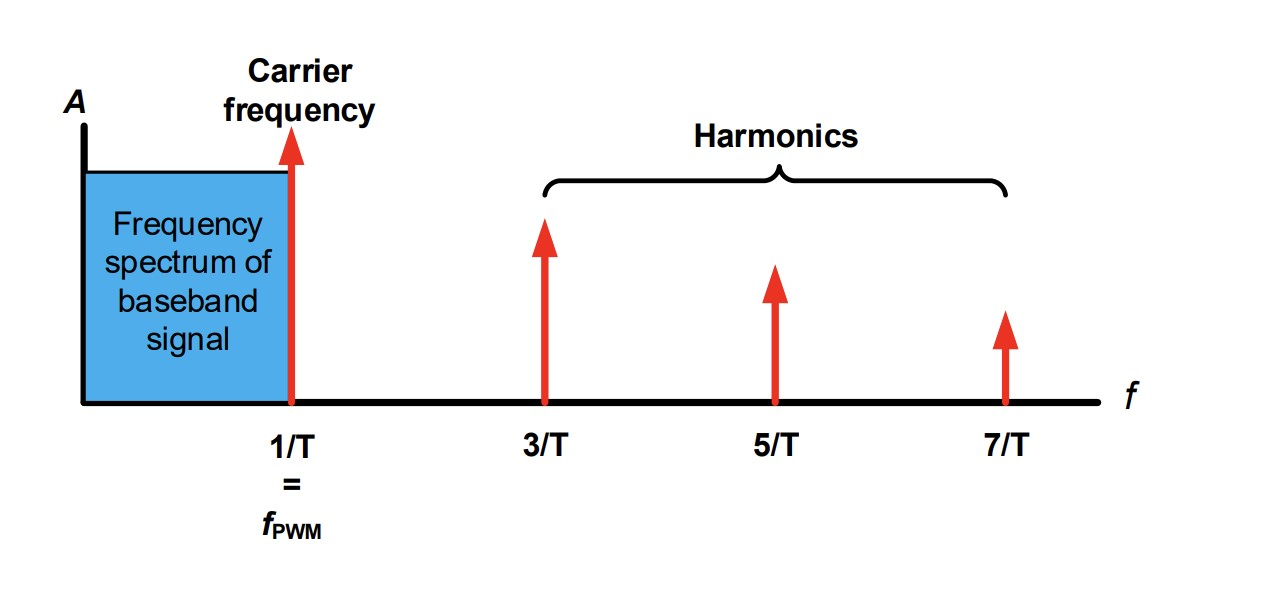
\includegraphics[width=1\linewidth]{pictures/pwm_spectrum_microchip90003250A.jpg}
    \caption{Spektrum PWM signálu převzatého od Microchip TB3250 kde $f_{PWM}$ je frekvence PWM signálu a $T$ je jeho perioda.}
    \label{fig:pwm_spectrum}
\end{figure}

Největší amplitudu typyckého PWM signálu má na její nastavené frekvenci $f_{PWM}$ a ostatní harmonické frekvence jsou její celočíselné násobky. Tyto frekvence přidávají nechtěný šum a můžou být potlačeny pomocí filtru typu dolní propust.


\begin{figure}[H]
    \centering
    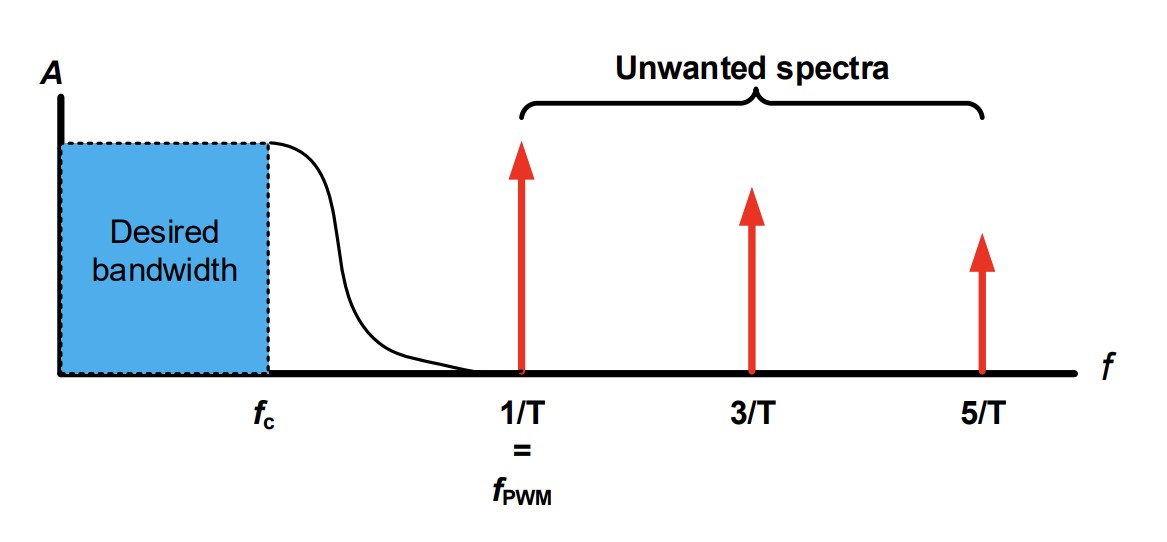
\includegraphics[width=1\linewidth]{pictures/rc_pwm_spectrum_microchip90003250A.jpg}
    \caption{Požadované odstraněné frekvence ve spektru PWM signálu převzatého od Microchip TB3250 kde $f_{PWM}$ je frekvence PWM signálu a $T$ je jeho perioda, $f_{c}$ je zlomová frekvence filtru.}
    \label{fig:unwanted_pwm_spectrum}
\end{figure}

Použitá dolní propust je RC filtr. Podle obrázku \ref{fig:variable_valve_driver} RC filtr je složený z odporu $R = 10 \ k\Omega$ a kondenzátoru $C = 100 \ nF$ kde výstupní napětí je napětí na kondenzátoru.
Kde $f_c = 159 \ Hz$ je zlomová frekvence filtru.

\begin{figure}[H]
    \centering
    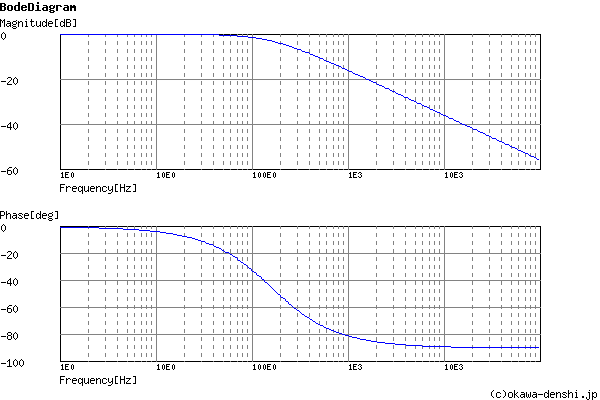
\includegraphics[width=1\linewidth]{pictures/var_rc_filter.png}
    \caption{Frekveční charakteristika použitého RC filtru. Obrázek je poskytnut z webové stránky \url{http://sim.okawa-denshi.jp/en/CRtool.php}}
    \label{fig:var_rc_filter_char}
\end{figure}

Na obrázku \ref{fig:var_rc_filter_char} můžeme vidět, že signál se začne atenuovat na zlomové frekvenci a fáze signálu se začne posouvat na frekvenci $\frac{f_c}{10}$.  \par

Aby výstupní řídící signál byl co nejvíce konstatní musíme zvolit vstupní frekvenci PWM signálu co nejvyšší, aby harmonické složky byly co nejvíce utlumeny.

\begin{figure}[H]
    \centering
    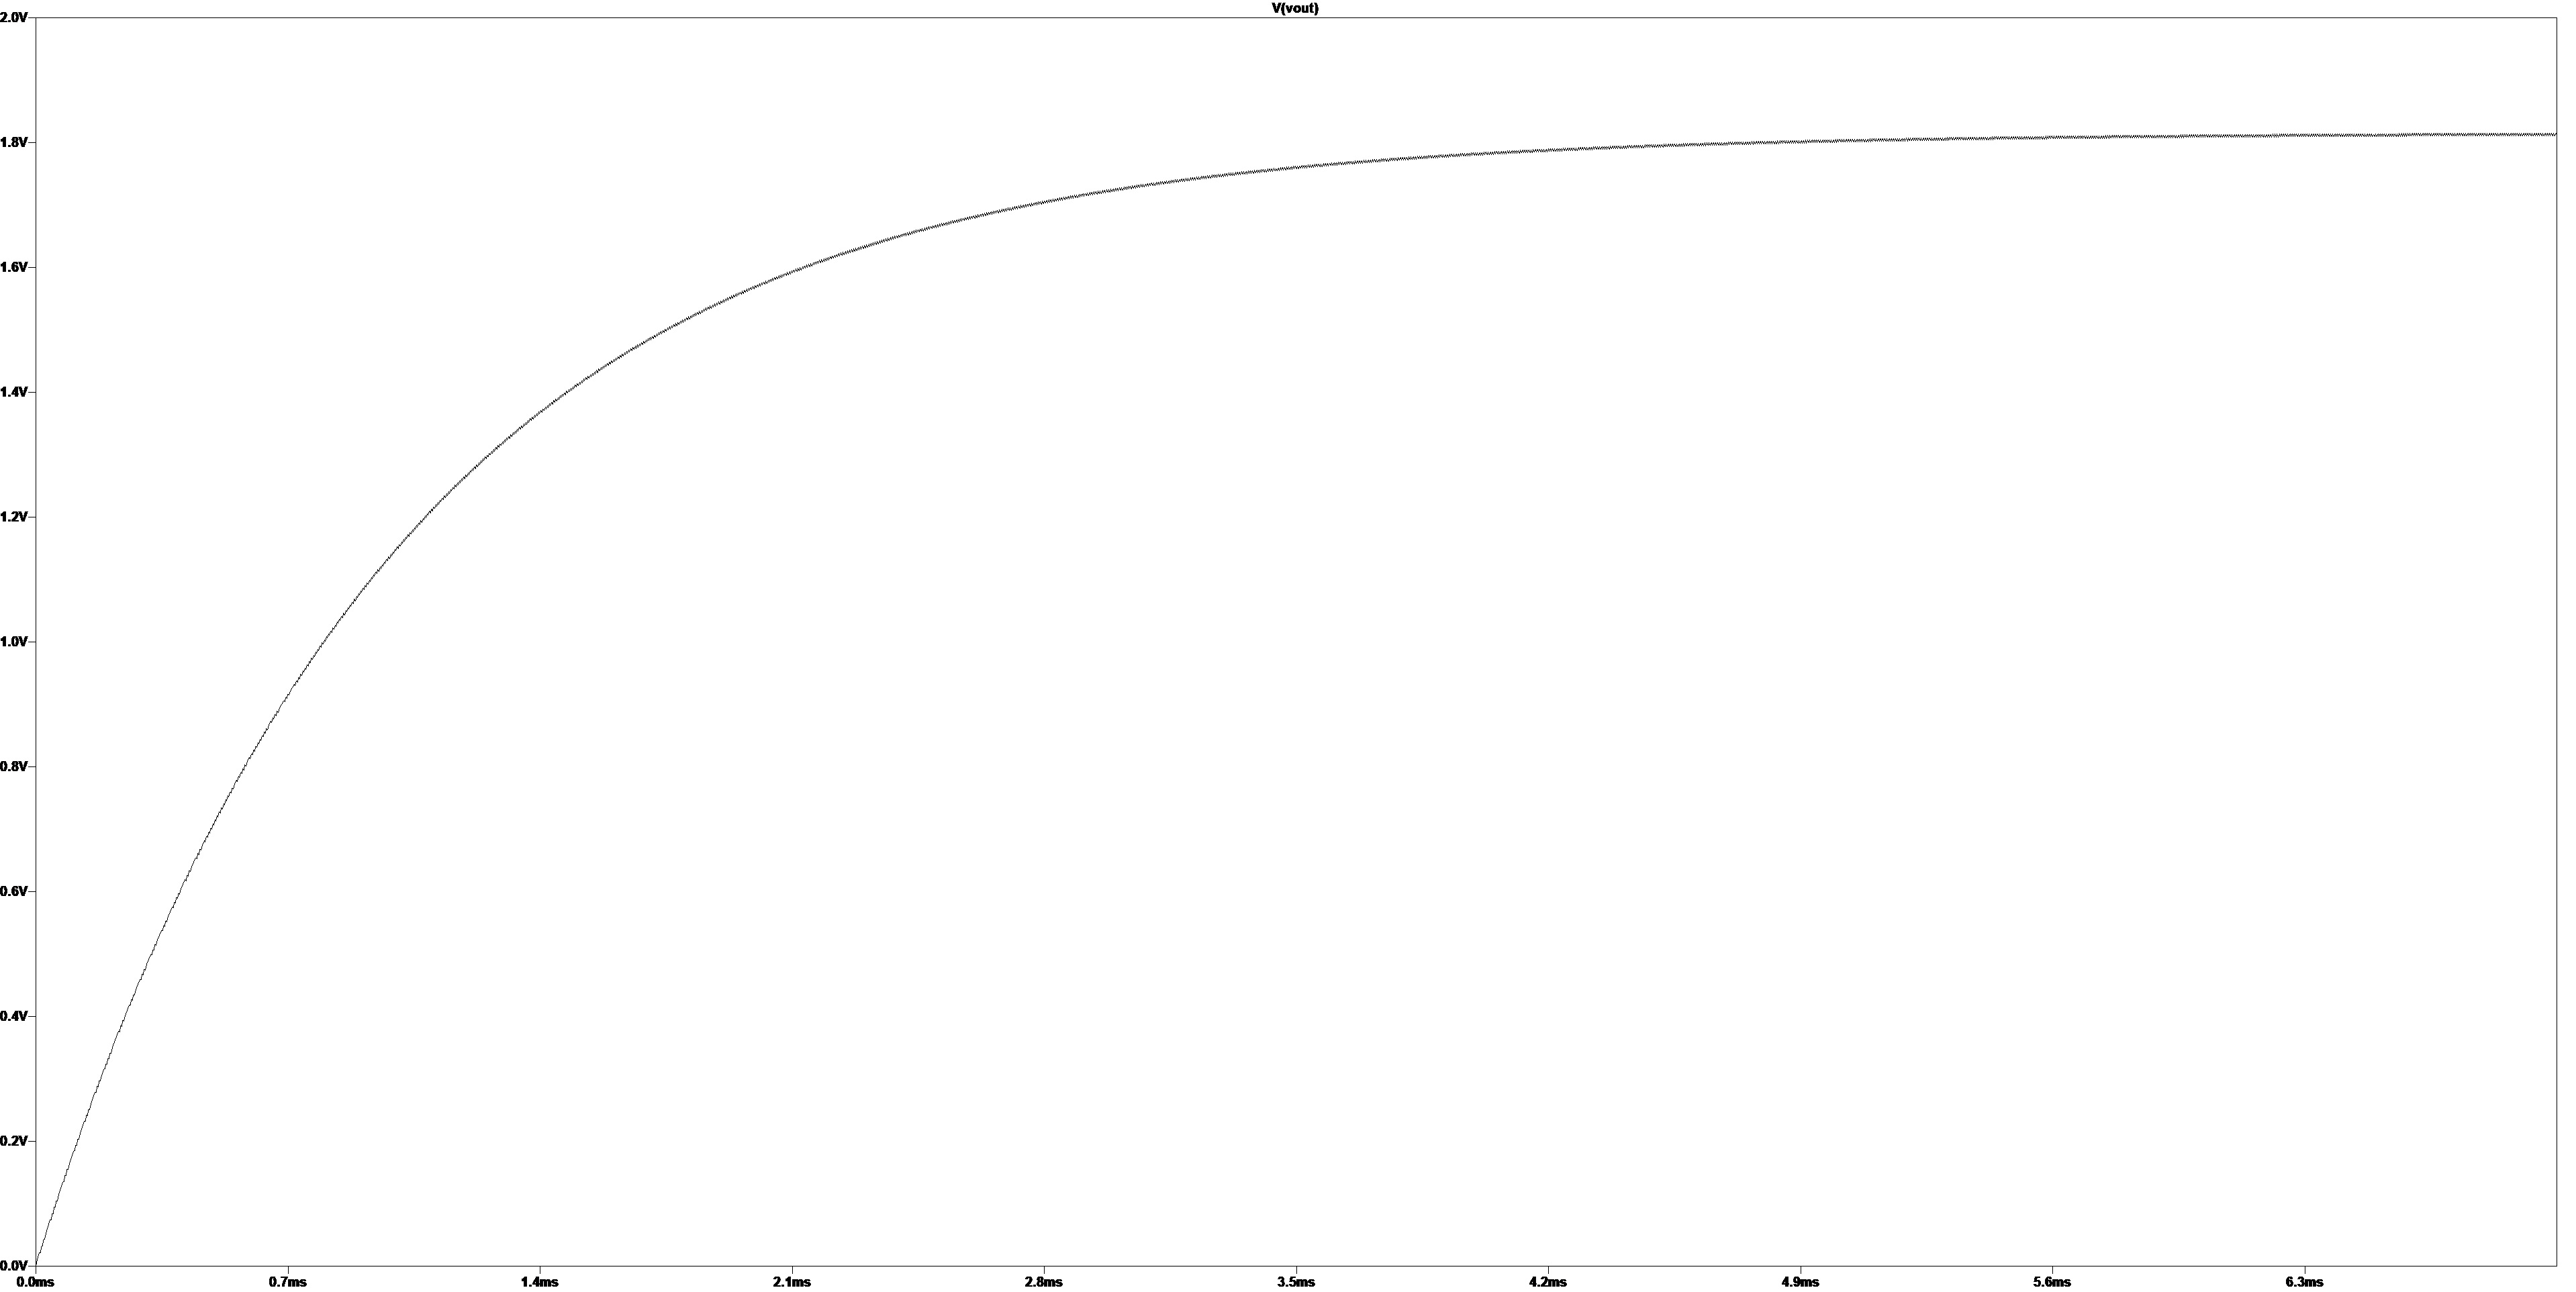
\includegraphics[width=1\linewidth]{pictures/filtered_pwm.jpg}
    \caption{Simulace RC filtru při vstupním PWM signálu o střídě $50\%$ a frekvencí $f_{PWM} = 168 \ kHz $. Simulace byla provedena v programu LTspice XVII.}
    \label{fig:filtered_pwm}
\end{figure}
Rušení výstupního signálu ovlivní chování regulačního ventilu. Toto rušení způsobí periodickou změnu amplitudy výstupního signálu a regulační ventil se podle této amplitudy bude periodicky otevírat a zavírat. Při zvolené frekvenci PWM $f_{PWM} = 168000 \ Hz $ je změna napětí $\approx 2 \ mV$. To způsobý změnu proudu $I = \frac{0.030}{25.5} = 11 \ mA $. \par
Volba velikosti prvků RC článku ovlivní schopnost reakce na změnu vstupního napětí.
Časová konstanta $\tau = RC = 10 \times 10^{3} \cdot 100 \times 10^{-9}= 1\ ms$ definuje čas, který potrvá aby napětí na kondenzátoru dosáhlo $U_{C}(\tau) = U_{in}(\tau)(1 - e^{-1})$, což je $\approx 63 \ \% $ vstupního napětí $U_{in}$.

\par
Díky rovnici
\begin{equation} \label{eq:pwm_accuracy}
    2^N = \frac{f_{TIMCLK}}{f_{PWM}}
\end{equation}
můžeme získat přesnost střídy PWM signálu. $f_{TIMCLK} = 168 \ MHz$ je obnovovací frekvence periferie TIMER, který generuje PWM signál. Pokud rovnici \ref{eq:pwm_accuracy} vyřešme pro $N$ získáme rovnici pro počet bitů a přesnosti střídy PWM signálu.
\begin{equation}
    N = \frac{\log_{2} (\frac{f_{TIMCLK}}{f_{PWM}})}{\log_{2}(2)} = \frac{ARR}{\log_{2}(2)}
\end{equation}
$ARR$ je Auto-Reload-Register MCU pro daný TIMER. Podle nastavené hodnoty v $ARR$ je možné nastavit frekvenci PWM signálu. Pro tento připad $N \doteq 9.96 $ bit.

\section{Digitalizace analogových signálů}
Tato sekce popisuje typy použitých analogově digitálních převodníků, které jsou použity pro snímání analogových výstupů ze senzorů tlaku. Jsou použity dva typy AD převodníků, první je 12 bit AD převodník součástí MCU SMT32F407ZG6 pro snímání napětí tlakových sezorů na větvých pneumatického systému popsaných v sekci \ref{section:pressure_sen}.
Další je 24 bit sigma-delta AD převodník Microchip MCP3561 pro snímání napětí z diferenčního tlakového sensoru popsaný v sekci \ref{section:diff_pressure_sen}.

\subsection{Snímání signálů z tlakových senzorů větvý pneumatíckého systému}
Je použit AD převodník součástí periférii rodiny MCU STM32F4xx. Jedná se o 12 bitový AD převodník s postunout aproximací a maximální vzorkovací frekvencí $f_{sample} = 2.4 \ MSPS$. Pro každý kanál se může aplikovat jiná vzorkovací frekvence. \par
Díky měření pouze absolutní hodnoty tlaku ze senzorů vzorkovací frekvence nemusí být vysoká. Vzorkovací frekvence je:
\begin{equation}
    f_{sample}=\frac{f_{ADCCKL}}{vzorkovací \, čas + 15 \, cyklů } = \frac{20.5 \! MHz}{480 + 15} \approx 41.5 \; kHz
\end{equation}
Vzorkovací frekvence závisí na vstupní frekvenci AD převodníku $f_{ADCCKL} = 20.5 \ MHz$, minimální počet $f_{ADCCKL} $ cyklů pro převod je $15$ a vzorkovacím časem, které jsou předem dané výrobcem. Minimální vzorkovací čas je $3$ a maximální je $480$.
\par
Přesnost AD převodníku je $1 LSB = \frac{U_{ref}}{2^N} = \frac{3.3}{2^{12}} = 0.000805 \ \frac{V}{ADC \ krok}$ závisí na referečním napětí diskutovaném v sekci \ref{section:vref}.

\begin{equation} \label{eq:max_adc_R}
    R_{AIN} = \frac{k - 0.5}{f_{ADCCLK} \cdot C_{ADC} \cdot ln(2^{N+2})} - R_{ADC}
\end{equation}
Rovnice \ref{eq:max_adc_R} slouží pro určení maximální vstupní externí impedance pro chybu pod $\frac{1}{4} \ LSB$. $N = 12$ je rozlišení AD převodníku, $k = 480$ je vzorkovací čas, $R_{ADC} = 6 \ k\Omega$ je vnitřní impedance vstupního kanálu AD převodníku a
$C_{ADC} = 4 \ pF$ je interní kapacita obvodu Sample and Hold. Výsledná maximální vstupní impedance je $R_{AIN} = 1.75 \ M\Omega$, ale podle katalogového listu je maximální externí impedance AD převodníku $R_{AIN} = 50 \ k\Omega$.
\par
K dalším chybám AD převodníku patří

\begin{table}[H]
    \label{tab:stm_adc_error}
    \caption{Přesnost ADC při $f_{ADC} = 30 \ MHz$}
    \hspace*{-1.3cm}
    \begin{ctucolortab}
        \begin{tabular}{ccccccc}
            \toprule
            Charakteristika               & Symbol & Testovací podmínky       & Typ       & $\textnormal{Max}^{(\ref{enum:stm_adc_max_ref})}$ & Jednotka & \\ \midrule
            Celková neupravená chyba      & $ET$   &                          & $\pm$ 2   & $\pm$ 5                                           &          & \\
            Napěťová nesymetrie           & $EO$   & $f_{ADC} = 30 \ MHz$     & $\pm$ 1.5 & $\pm$ 2.5                                         &          & \\
            Napěťový zisk                 & $EG$   & $R_{AIN} < 10 \ k\Omega$ & $\pm$ 1.5 & $\pm$ 3                                           & LSB      & \\
            Difereciální  chyba linearity & $ED$   &                          & $\pm$ 1   & $\pm$ 2                                           &          & \\
            Integrální chyba linearity    & $EL$   &                          & $\pm$ 1.5 & $\pm$ 3                                           &          & \\
            \bottomrule
        \end{tabular}
    \end{ctucolortab}
    \begin{enumerate}
        \item \label{enum:stm_adc_max_ref} Maximální tlak, který může být aplikován na jeden z portů senzoru a zachoval původní specifickace.
    \end{enumerate}
\end{table}

\subsection{Snímání signálů z diferenčního tlakového sensoru pneumatíckého systému}
Difereční sensor tlaku snímá dynamické jevy tlaku krevního řečiště. Tlaková vlna má frekvenci $f = x \ Hz$ XXXXX SEM DOPLNIT. Aby byla tlaková vlna správně převedena do digitálního signálu, musí být dodržen Nyquistův teorém.
\begin{equation} \label{eq:nyquist}
    f_s \geq 2f
\end{equation}
Rovnice \ref{eq:nyquist} říká, že vzorkovací frekvence musí být alespoň dvojnásobek snímaného signálu.
\par
Byl vybrán 24 bit sigma-delta AD převodník MCP3561 od firmy Microchip s maximální vzorkovací frekvencí $153.6 \ kHz$. Je to AD převodník s velmi nízkým šumem, s jedním diferečním vstupem nebo dvěmi jednotlivými vstupy analogových signálu.
Obsahuje interní oscilátor, teplotní sensor, obvody pro detekci zkratu či odpojeného sensoru, programovatelné zesílení od $0.33 \times$ až $64 \times$ a další.
\par
MCP3561 komunikuje s MCU pomocí komunikačního rozhraní Serial Peripheral Interface (SPI) až s maximální rychlostí $20 \ MHz$. Komunikace probíha po 8 bitových slovech, kde odpovědi z AD převodníku můžou mít délku 8,24 a nebo podle kofigurace i 32 bit.
\begin{figure}[H]
    \centering
    \caption{Zapojení AD převodníku MCP3561}
    \label{fig:mcp3561_connection}
    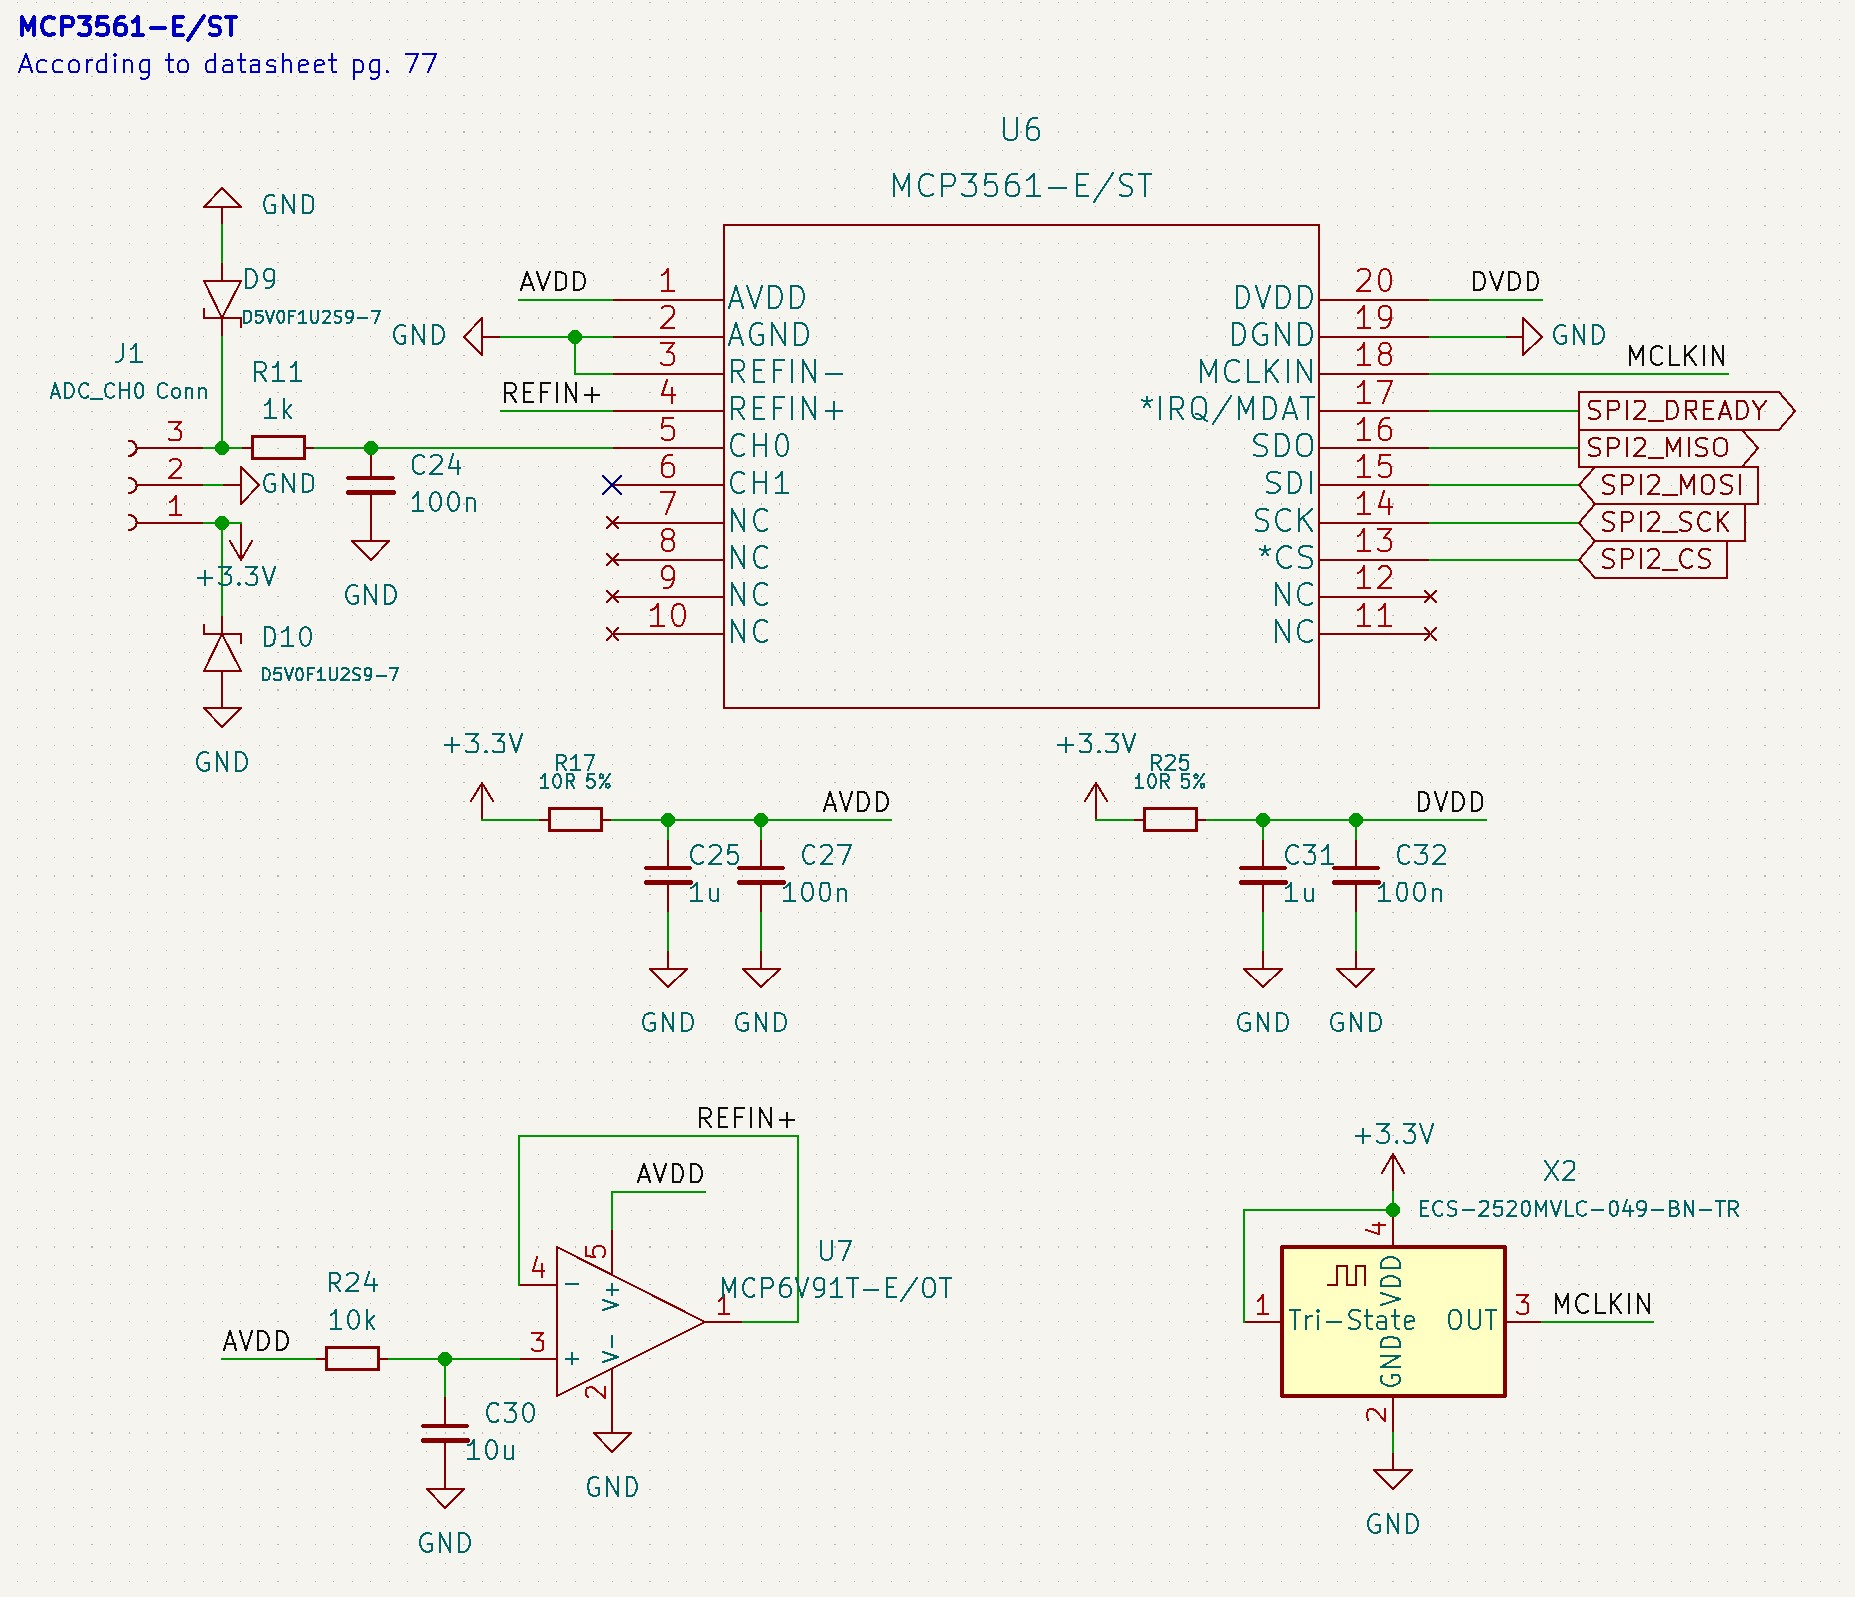
\includegraphics[width=1\linewidth]{pictures/mcp3561_connection.jpg}
\end{figure}
Na obrázku \ref{fig:mcp3561_connection} je schéma zapojení MCP3561 podle doporučeného zapojení výrobce.
\subsubsection{Napájení a napěťové reference}
Zapojení obsahuje oddělené filtrování analogového a digitálního napajecího vstupu.
Referenční napájení AD převodníku obsahuje operační zesilovač v zapojení napěťového sledovače, protože vstupní reference AD převodníku není impedančně oddělená. Operační zesilovač je MCP6V91T od firmy Microchip. Má nízkou teplotně závislou napětovou nesymetrii $U_{OS \ Drift} = \pm 17  \ \frac{nV}{^\circ C}$
a také nízkou napěťovou nesymetrii $U_{OS} = 9 \ \mu V$, nízký šum a je optimalizovaný pro použití v prostředí s vysokým elektromagnetickým prostředí.

\subsubsection{Externí oscilátor}
Místo interního oscilátoru AD převodníku je použit externí oscilátor ECS-2520MVLC od firmy ECS Inc. s frekvencí $f_{CLK} = 4.9152 \ MHz$. Externí oscilátor zaručí stabilní funkčnost AD převodníku, protože přesnost interního oscilátoru není výrobcem zaručena, rozdíly až $\pm 30  \ \%$, může se lišit čip od čipu, mohou způsobit vadnou komunikaci a další nepredikovatelné chování.
Podporované frekvence externího oscilátoru jsou v rozmezí $ 1 \ MHz \leq  f_{CLK} \leq 20 \ MHz $. Frekvence $f_{CLK} = 4.9152 \ MHz$ byla zvolena díky naměřených parametrů AD převodníku v katalogovém listu právě při použití této frekvence.
\par
Maximální možná vzorkovací frekvence pro tuto frekvenci oscilátoru je $f_s = 38400 \ Hz$.

\subsubsection{Přesnost a rušení}
Nejmenší možné snímané napětí ideálního $N = 24$ bit AD převodníku při referečním napětí $U_{ref} = 3.3 \ V $ je $ 1 \ LSB = \frac{U_{ref}}{2^{N}} \doteq  196,695  \ nV$.
Efektivní počet bitů (ENOB) závisí na interní konfiguraci registrů MCP3561 a od toho se také odvíjí jakou vzrokovací frekvenci můžeme mít. Rovnice pro výpočet vzorkovací frekvence je
\begin{equation}
    f_s = \frac{f_{CLK}}{4 \times OSR \times Prescale}
\end{equation}

\section{Napájení}
Vstupní napájení je použito pro napájení celého přistroje. Vstupní napětí je $U_{in} = 5V DC$, které poskytuje napájení pro všechny součástky na přístroji. Vstupní napětí je poté pomocí regulátoru napětí s nízkým úbytkem usměrněno na $3.3 V$ pro napájení MCU, sensorů a ostatních komponentů.

\begin{figure}[H]
    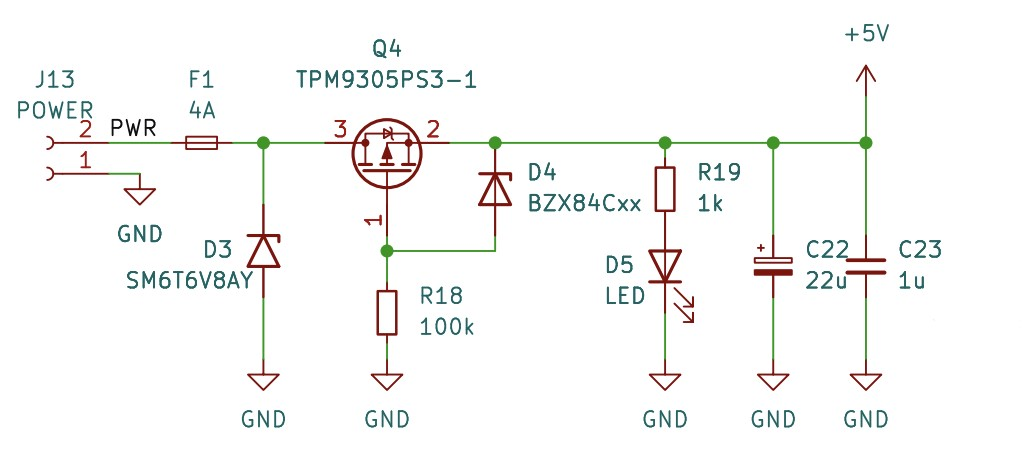
\includegraphics[width=0.9\linewidth]{pictures/power.jpg}
    \caption{Schéma zapojení vstupního napájení}
    \label{fig:power_input}
\end{figure}

Celkový proudový odběr přístroje je .....

Přístroj je opatřen $4 [A]$ pojistkou a ochranou proti opačné polaritě.
Ochrana proti opačné polaritě zajistí při špatném zapojení, aby proud neprotékal přístrojem, ale musí se zajistit, aby ztrátový výkon
\begin{align*}
    W = I^2 R
\end{align*}

byl co nejmešní při správném zapojení. Proto je použit PMOS tranzistor jako ochrana obvodu, který . Gate tranzistoru je připojena k zemi a mezi Drain a Source protéká proud při správném zapojení napájecího zdroje. Protože $ U_G = 0 [V]$ a $U_S = U_{in}$, tak
\begin{align*}
    U_{GS} = U_G - U_S
\end{align*}
$U_{GS} = -U_{in} $, proto je potřeba, aby
\begin{align*}
    U_{GS(ON)} > -U_{in}
\end{align*}
Při opačném zapojení napájení $U_S = -U_{in}$ a $ U_G = 0 V$, tak  $U_{GS} = U_{in}$ tranzistor je vypnut a přes obvod neprotéká proud.
V návrhu je použit tranzistor TPM9305PS3, který má  $U_{GS(ON)} = -2.5V $,  $I_D = -4.1A$ a $R_{DS(ON)} = 52m \Omega$ při $U_{GS} = -4.5V$.
Ztrátový výkon bude
\begin{align*}
    W_{loss} = I^2 R \approx (3)^2 (0.053) =  159 mW
\end{align*}

Na obrázku \ref{fig:power_input} je ještě připojena mezi $U_G$ a $U_S$ zenerova dioda, která zamezí maximální napětí, pro ochranu tranzistoru. Pokud napájecí zdroj bude mít větší napětí něž maximální povolené napětí na $U_{GS}$, zenerova dioda upne $U_{GS}$ na její maximální napětí.
\par
Pro maximální zamezení rušivých jevů a braní ohledu na EMC jsou připojeny paralelně dva blokovací kondenzátory.

\begin{figure}[H]
    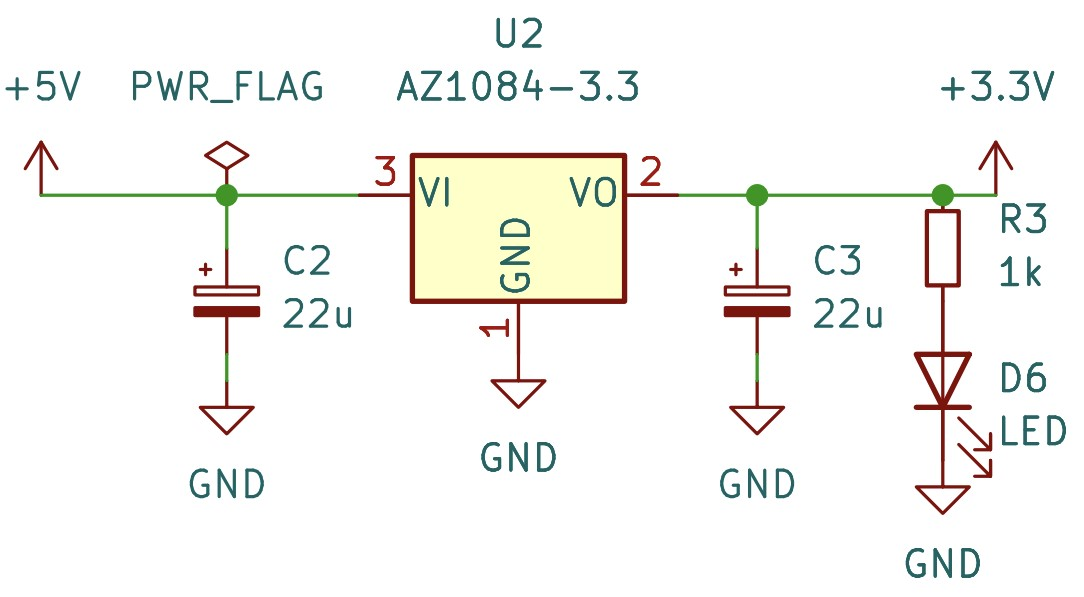
\includegraphics[width=0.9\linewidth]{pictures/ldo_3v3.jpg}
    \caption{Schéma zapojení regulátoru napětí z 5V na 3.3V}
    \label{fig:stepdown}
\end{figure}
Na obrázku \ref{fig:stepdown} je schéma zapojení lineárního regulátoru napětí s nízkým úbytkem AZ1083-3.3. Vstupní napětí je v rozmezí $1.5V \leq U_{in} \leq 12V $. Výstup regulátoru je fixní na $U_{out} = 3.3V$ a maximální výstupní proud je $I_{out(MAX)} = 5A$. Zapojení regulátoru je podle doporučeného zapojení v datasheet.


%Software
%!TEX ROOT=main.tex
\chapter{Software}
%Results
%!TEX ROOT=main.tex
\chapter{Implementace}
V této kapitole je popsaná realizace systému CarDi a naměřené hodnoty pneumatického systému.

\section{Deska plošného spoje}
Na desce plošného spoje (DPS) sídlí všechny elektrické komponenty systému. DPS a schéma je navržena v otevřeném freeware KiCad EDA.
\begin{figure}[H]
    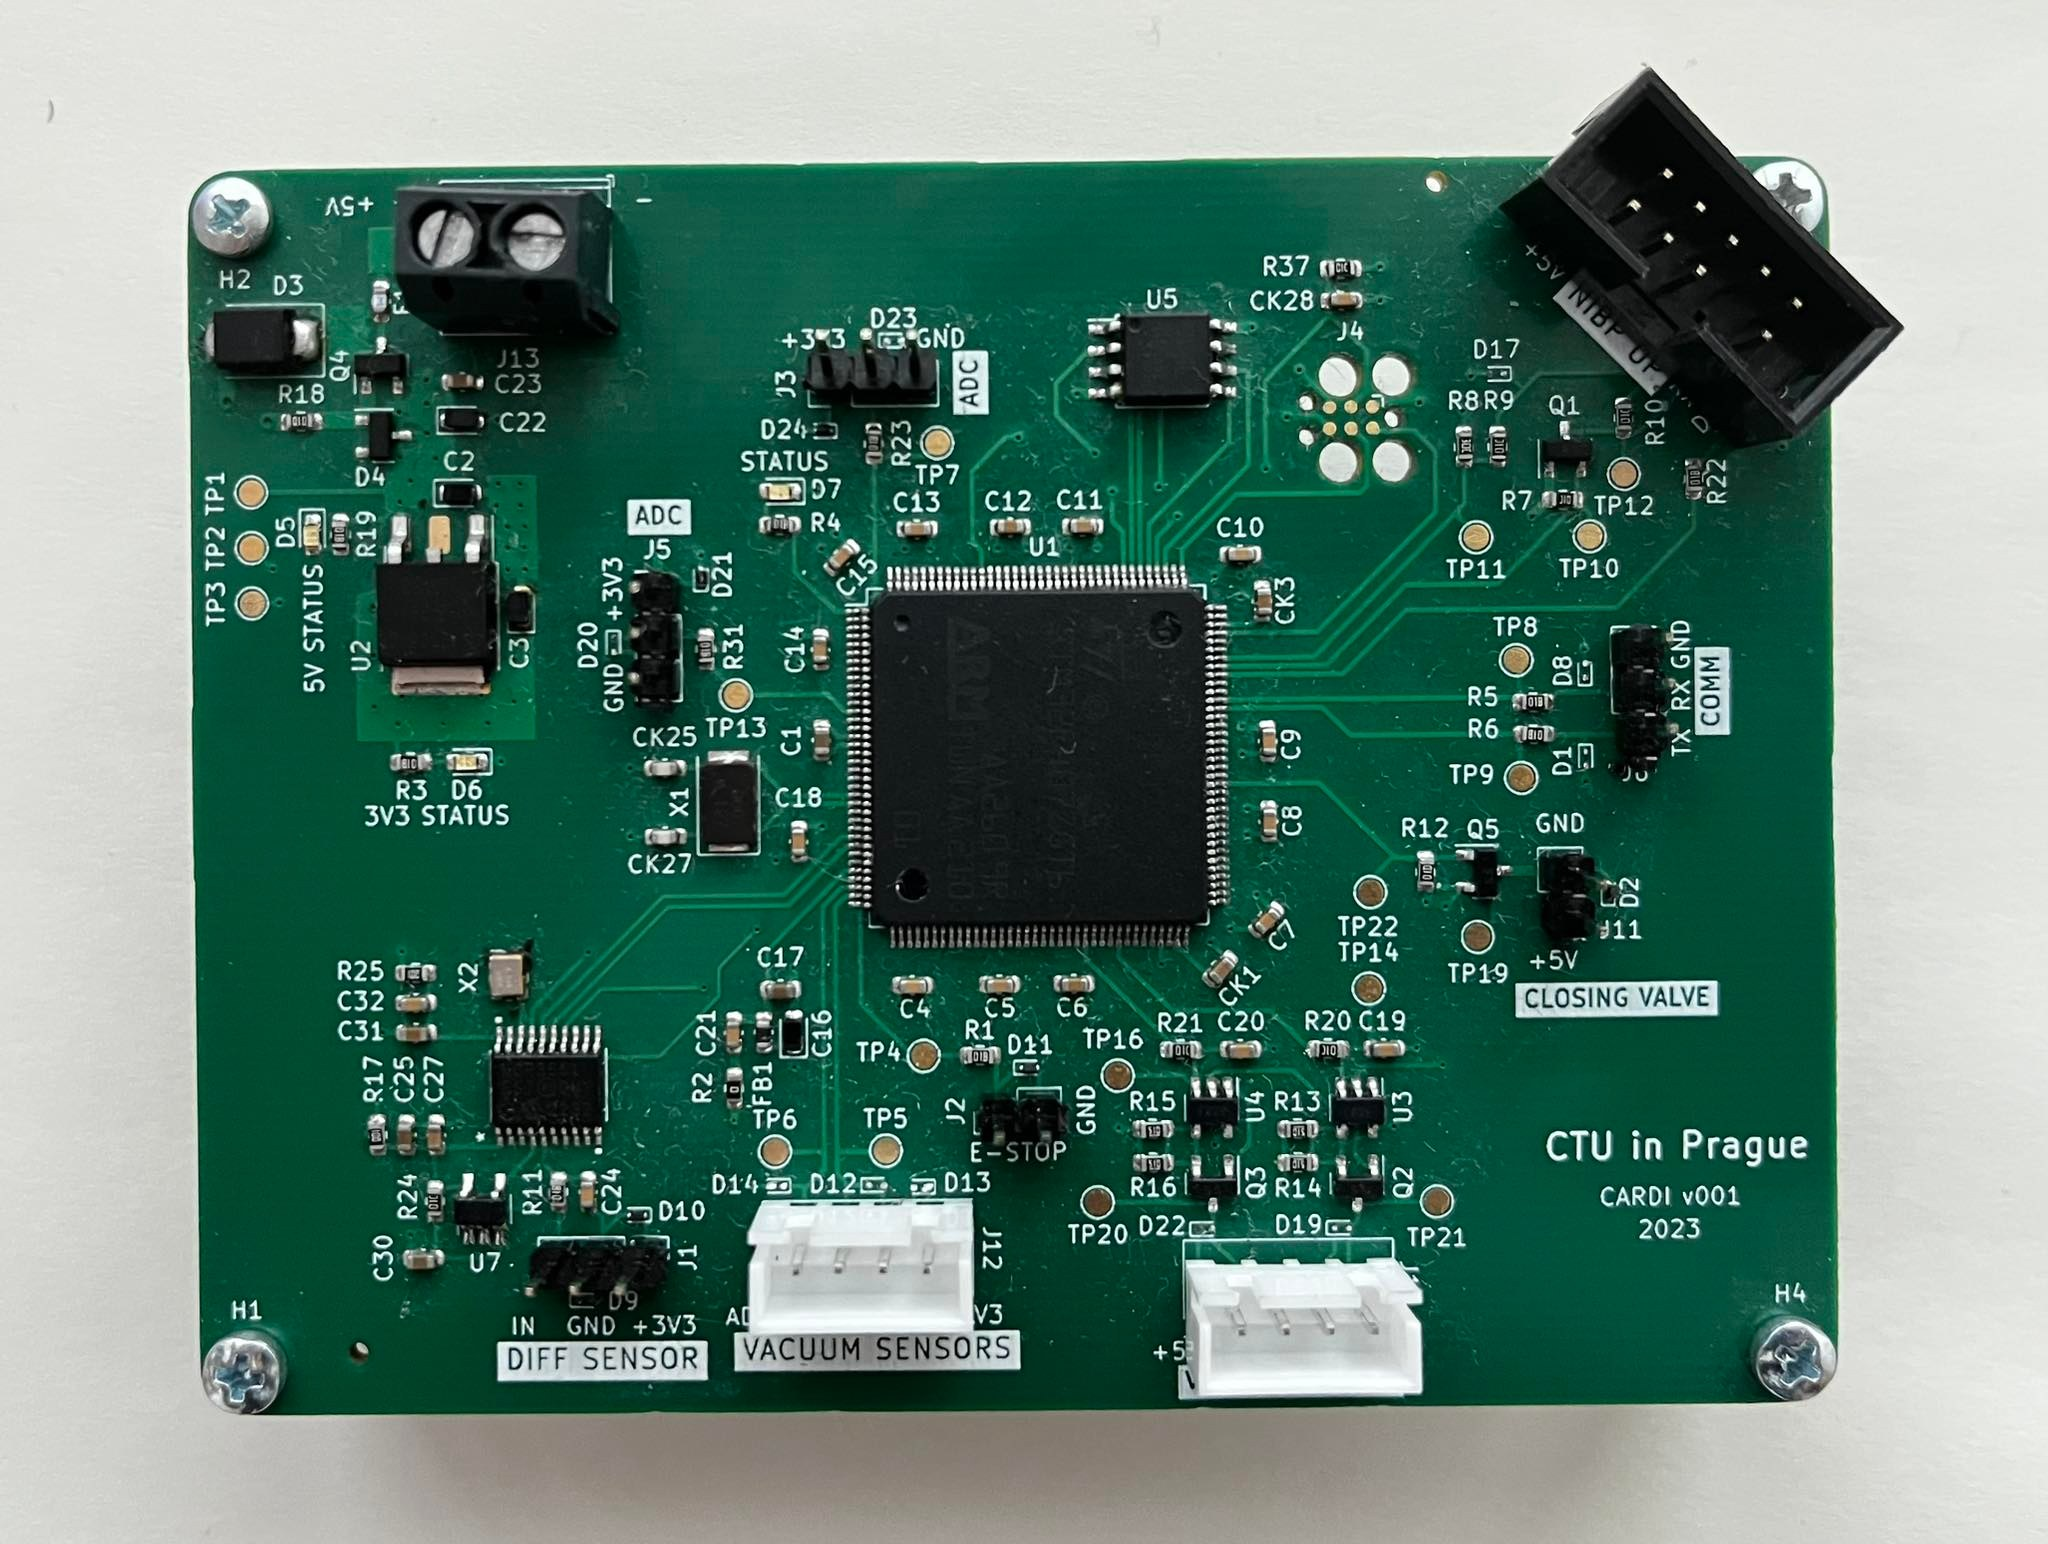
\includegraphics[width=1\linewidth]{pictures/pcb_full.jpg}
    \caption{Realizovaná deska plošného spoje.}
    \label{fig:pcb_full}
\end{figure}

DPS je čtyřvsrtvá deska s dvěma signálovými vrstvy a dvěma silovýma vrstvama. Kde první(horní) vrstva je signálová a nachází se na ní veškeré elektronické komponenty. Druhá je společná zem, třetí je napájencí 3.3 V a poslední spodní vrtva je také signálová.
Základní materiál je FR-4 a povrchová úprava je ENIG(Electroless nickel immersion gold).
\par
DPS je vyrobena a z části osazena firmou JLCPCB.
\begin{figure}[H]
    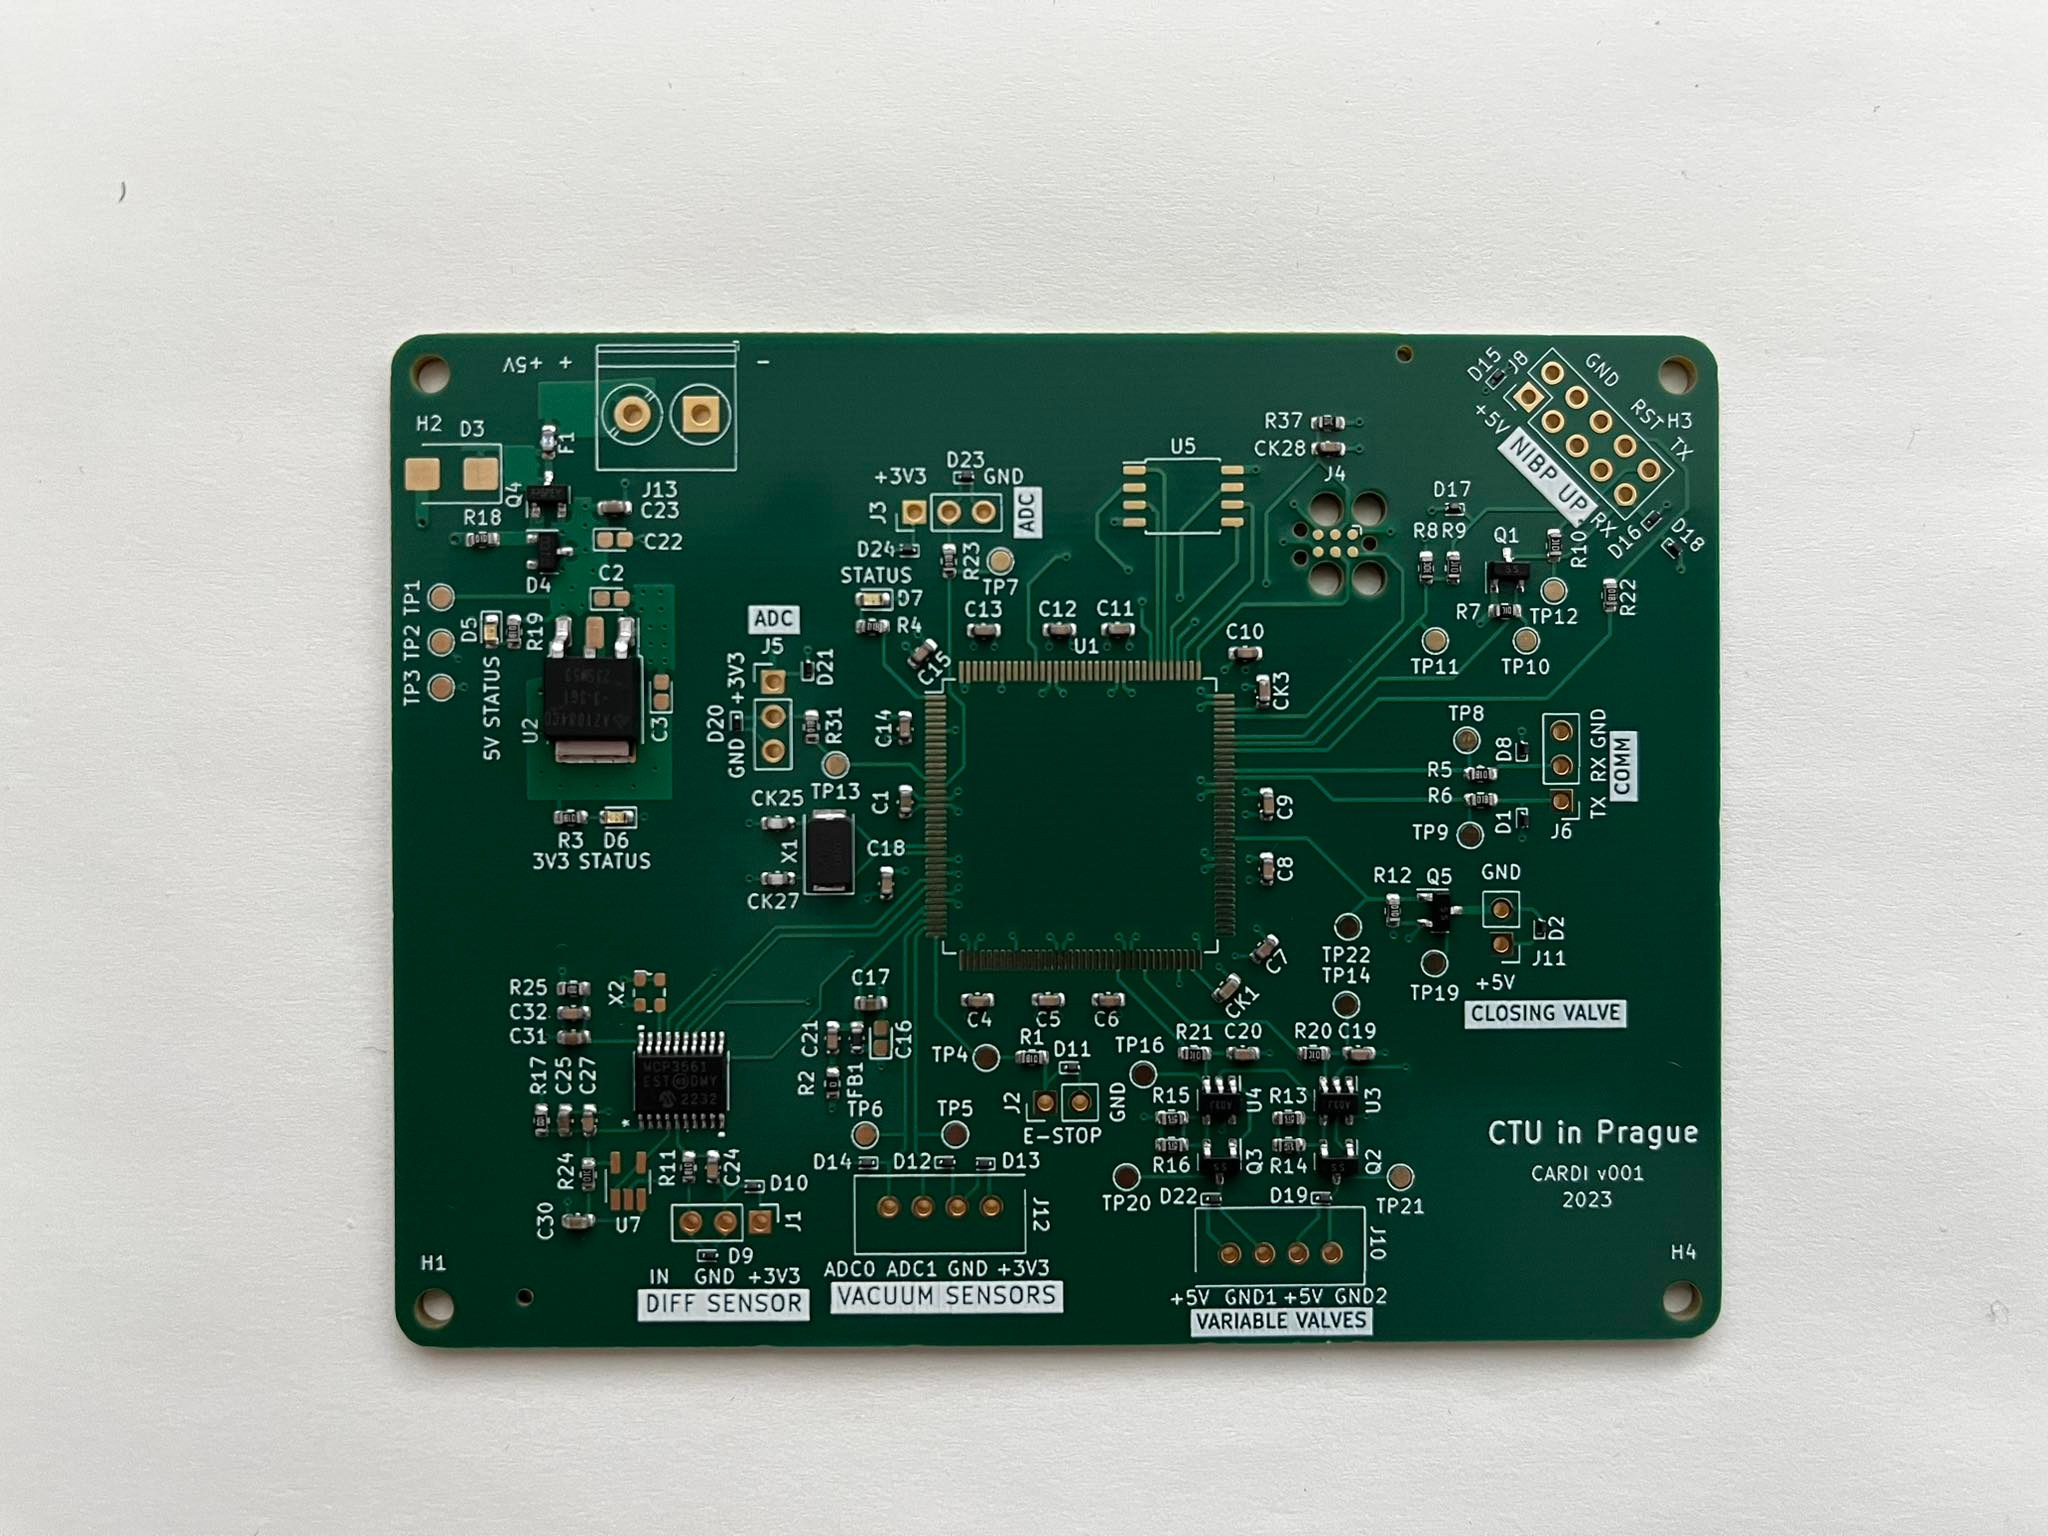
\includegraphics[width=1\linewidth]{pictures/pcb_from_production.jpg}
    \caption{Deska plošného spoje z výroby.}
    \label{fig:pcb_production}
\end{figure}
\begin{figure}[H]
    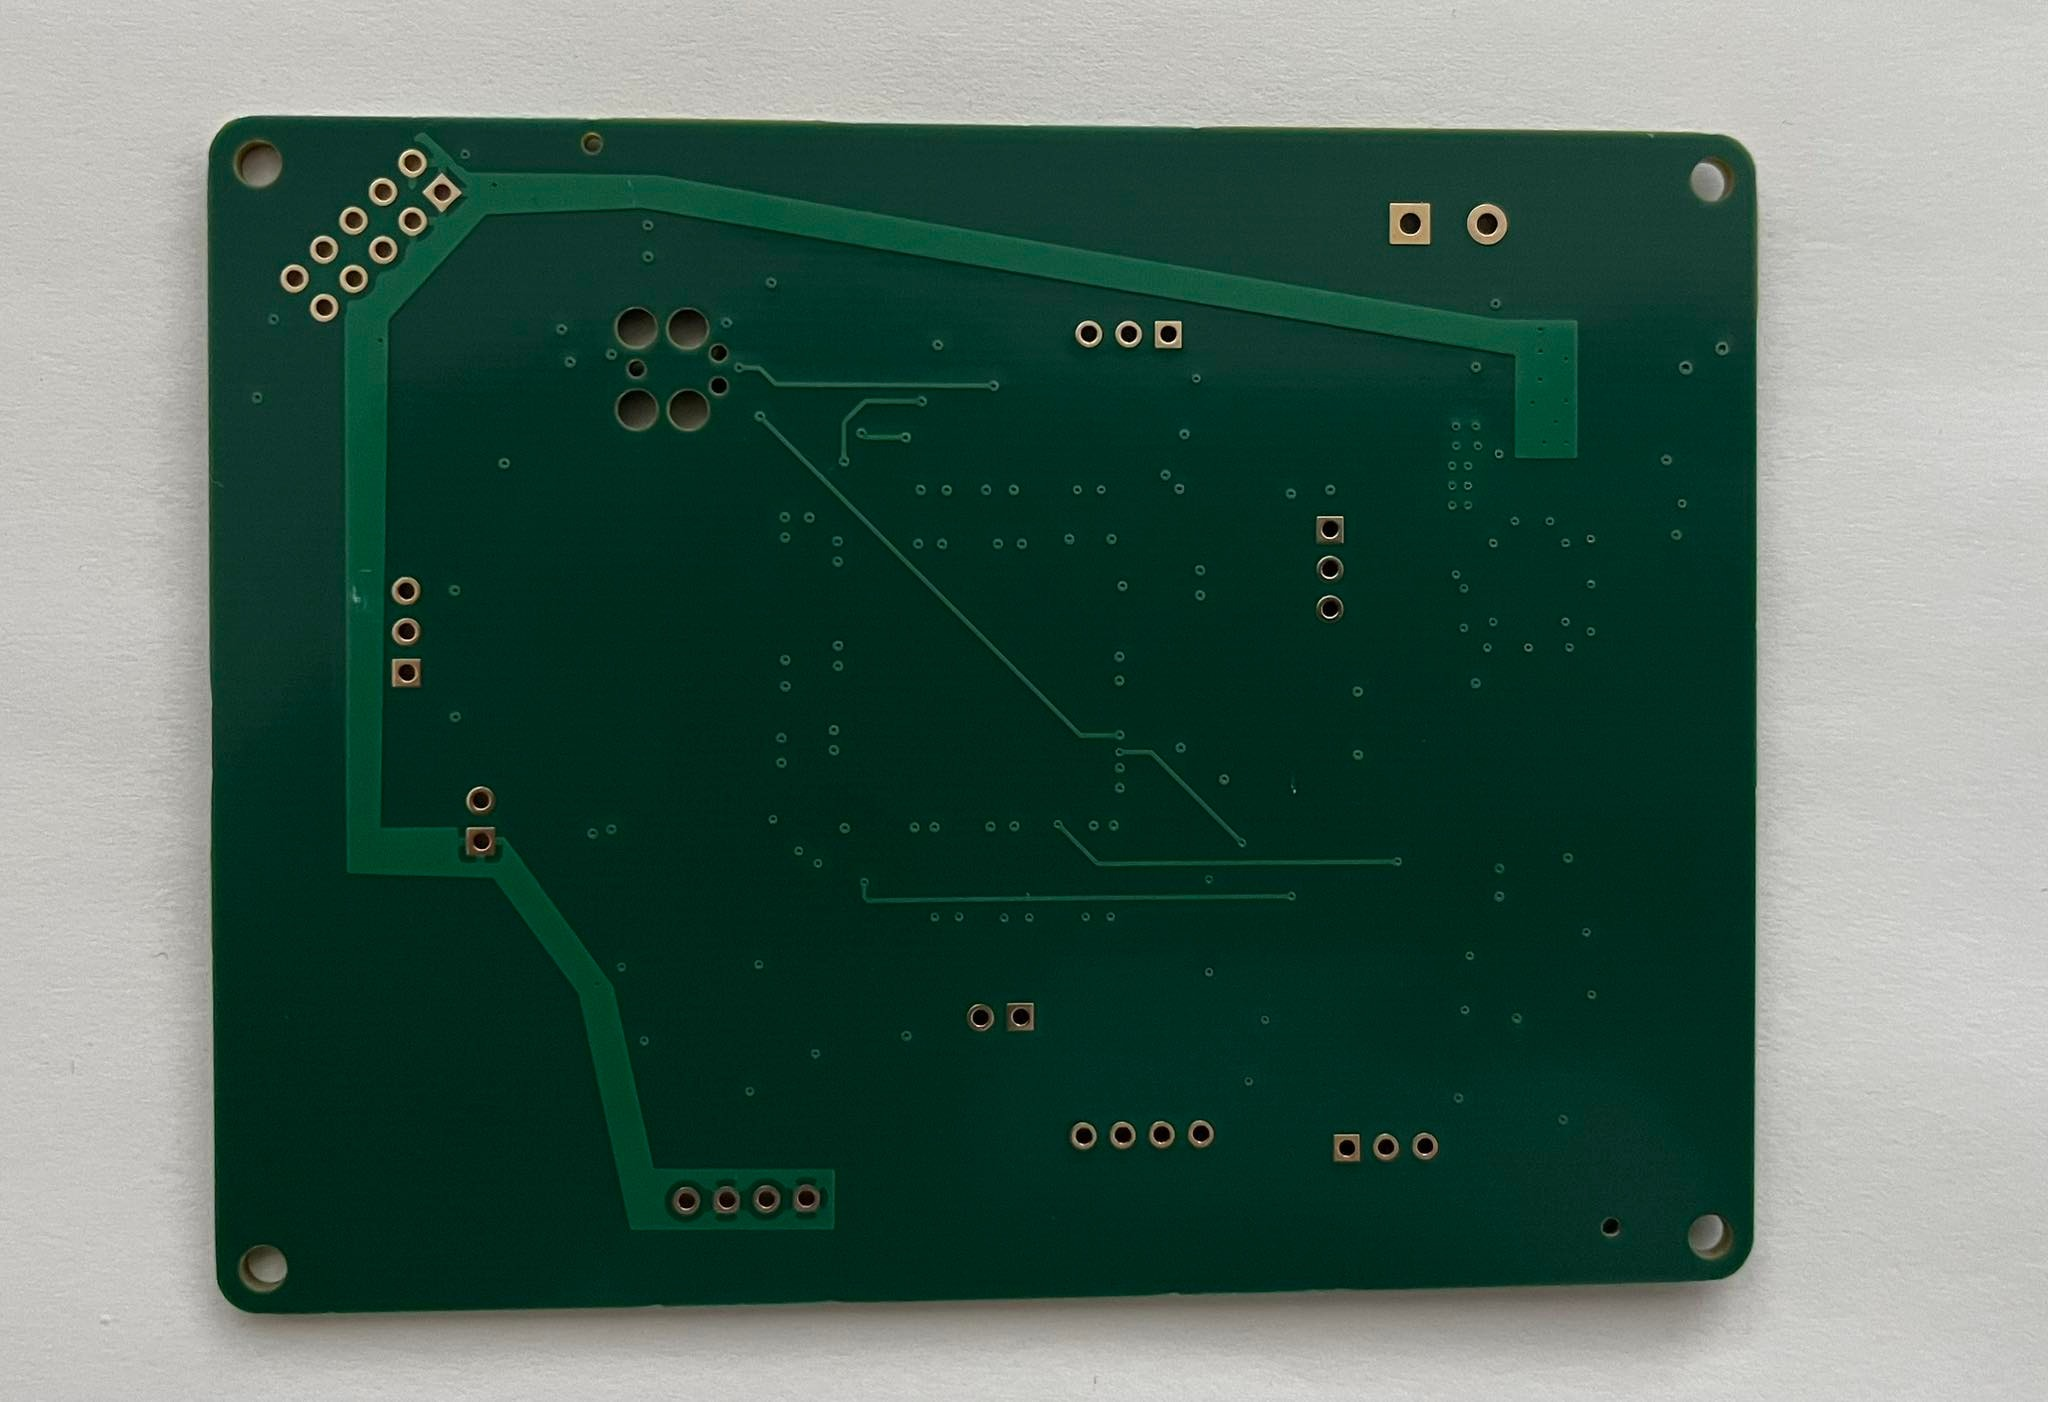
\includegraphics[width=1\linewidth]{pictures/pcb_production_bottom.jpg}
    \caption{Deska plošného spoje z výroby. Spodní vrstva.}
    \label{fig:pcb_production_bottom}
\end{figure}

Celkovká cena desky a potřebné materiály jsou:

\begin{table}[H]
    \label{tab:bom}
    \caption{Celkový počet součástek a výrobní cena }
    \begin{ctucolortab}
        \begin{tabular}{ccccccc}
            \toprule
            Typ                   & Název                  & Hodnota       & Počet & Cena     & Jednotky & \\ \midrule
            Kondenzátor           &                        & 100 nF        & 10    & 0.022    &          & \\
            Kondenzátor           &                        & 22 pF         & 2     & 0.0174   &          & \\
            Kondenzátor           &                        & 1 uF          & 4     & 0.018    &          & \\
            Kondenzátor           &                        & 2.2 uF        & 2     & 0.0096   &          & \\
            Kondenzátor           &                        & 4.7 uF        & 1     & 0.0091   &          & \\
            Kondenzátor           &                        & 10 uF         & 1     & 0.006    &          & \\
            Kondenzátor           &                        & 22 uF         & 3     & 0.015    &          & \\
            Resistor              &                        & 51 $\Omega$   & 4     & 0.5688   &          & \\
            Resistor              &                        & 10 $\Omega$   & 2     & 0.0032   &          & \\
            Resistor              &                        & 20 $k\Omega$  & 5     & 0.005    &          & \\
            Resistor              &                        & 10 $k\Omega$  & 7     & 0.0056   &          & \\
            Resistor              &                        & 0 $\Omega$    & 1     & 0.001    &          & \\
            Resistor              &                        & 1 $k\Omega$   & 10    & 0.005    &          & \\
            Resistor              &                        & 100 $k\Omega$ & 2     & 0.002    & €        & \\
            Dioda                 & BZX84C10VLT116         &               & 1     & 0.2264   &          & \\
            Dioda                 & D5V0F1U2S9-7           &               & 19    & 3.0837   &          & \\
            Dioda                 & SM6T6V8AY              &               & 1     & 0.1372   &          & \\
            Dioda                 & LED Green              &               & 3     & 0.0717   &          & \\
            IO                    & AZ1084CD-3.3TRG1       &               & 1     & 0.2395   &          & \\
            IO                    & MCP3561-E/ST           &               & 1     & 5.5941   &          & \\
            IO                    & MCP6001RT-I/OT         &               & 2     & 0.486    &          & \\
            IO                    & MCP6V91T-E/OT          &               & 1     & 1.81     &          & \\
            IO                    & MX25R3235FM2IL0        &               & 1     & 0.88     &          & \\
            IO                    & STM32F407ZGT6          &               & 1     & 1.02     &          & \\
            MOSFET                & TPM9305PS3-1           &               & 1     & 0.0958   &          & \\
            MOSFET                & BSS138                 &               & 4     & 0.09     &          & \\
            Ferritový korálek     & MPZ1608S102ATA00       &               & 1     & 0.0196   &          & \\
            Oscilátor             & ABM3-8.000MHZ-D2Y-T    & 8 MHz         & 1     & 0.5783   &          & \\
            Oscilátor             & ECS-2520MVLC-049       & 4.9152 MHz    & 1     & 1.23     &          & \\
            Pojistka              & F0603FF4000V032TM      & 4 A           & 1     & 0.0762   &          & \\
            \bottomrule
            $\Sigma$              &                        &               & 94    & 16.3262  & €        & \\
            \bottomrule
            Služba                & Výroba PCB od JLCPCB   &               & 1     & 5        & €        & \\
            Služba                & Osazení PCB            &               & 1     & 16       & €        & \\
            \bottomrule
            $\Sigma$              &                        &               & 2     & 21       & €        & \\
            \bottomrule
            Programátor           & ST-LINK/V2-ISOL        &               & 1     & 76.99    & €        & \\
            Kabel na programování & Tag Connect TC2030 IDC &               & 1     & 40.37    & €        & \\
            \bottomrule
            $\Sigma$              &                        &               & 2     & 117.36   & €        & \\
            \bottomrule
            \bottomrule
            $\Sigma$              & Bez DPH                &               &       & 154.6862 & €        & \\
            \bottomrule
        \end{tabular}
    \end{ctucolortab}
\end{table}
\section{Pneumatická část}

Pneumatická čast systému je část ve které probíhá měření měření hemodynamických parametrů srdce pacienta. Je to jediná čast systému, která přichází v přímý kontakt s pacientem.
\begin{figure}[H]
    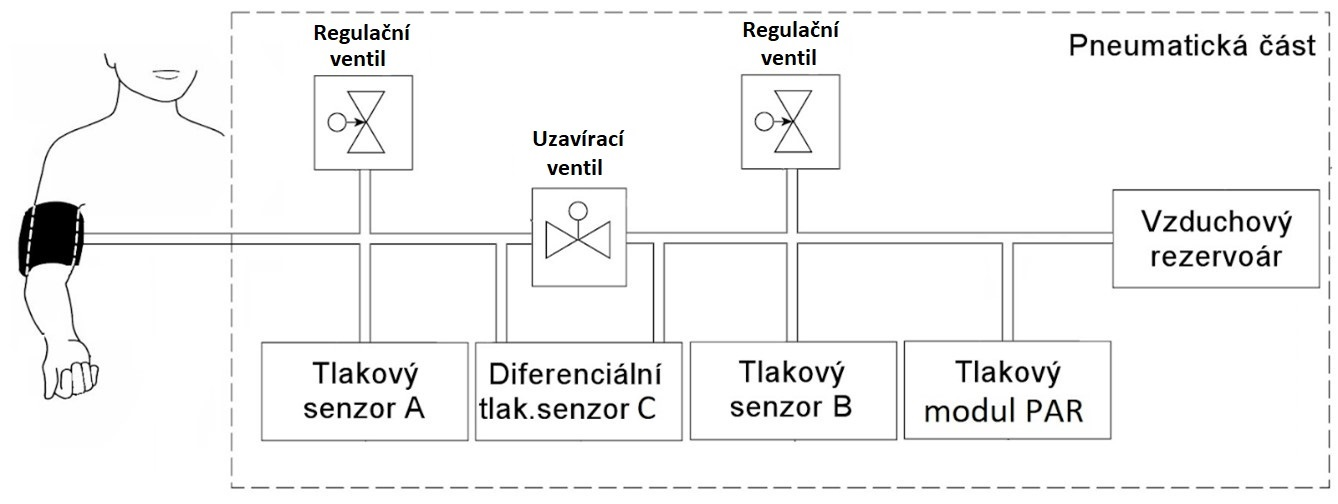
\includegraphics[width=1\linewidth]{pictures/blokove_schema_pneu.jpg}
    \caption{Blokové schéma pneumatického systému}
    \label{fig:pneu_block}
\end{figure}

\subsection{Měření těsnosti penumatické časti}
Pneumatická čast musí být co nejlépe těsná, aby po dobu terapie byl co nejmešní úbytek tlaku v systému.
\par
Test těsnosti probíhal pomocí přístroje FLUKE Biomedical BP pump 2, který natlakoval pneumatickou část na hodnotu 200 mmHg a následně sledoval úbytek tlaku v systému po dobu 60 s.
Měření bylo opakováno 10 krát po sobě.

\begin{table}[H]
    \label{tab:pressure_test_pneu}
    \caption{Test těstnosti pneumatického systému}
    \begin{ctucolortab}
        \begin{tabular}{ccc}
            \toprule
            Měření & Těsnost & Jednotky           \\ \midrule
            1      & 0.9     &                    \\
            2      & 0.8     &                    \\
            3      & 1.1     &                    \\
            4      & 1.0     &                    \\
            5      & 0.9     & $\frac{mmHg}{min}$ \\
            6      & 0.9     &                    \\
            7      & 1.1     &                    \\
            8      & 0.9     &                    \\
            9      & 0.8     &                    \\
            10     & 1.0     &                    \\
            \bottomrule
        \end{tabular}
    \end{ctucolortab}
\end{table}
Průměrný pokles tlaku v důsledku úniku vzduchu z pneumatického obvodu je $0.94 \ \frac{mmHg}{min}$ se směrodatnou odchylkou $0.10  \ \frac{mmHg}{min}$. Dle normy je maximální úbytek tlaku v systému $4 \ \frac{mmHg}{min}$.
\subsection{Zkreslení signálu pneumatickým systémem}
Přenosová funkce systému byla identifikována měřením impulzní odezvy systému. Systém byl natlakovám na průměrnou hodnotu suprasystolického tlaku 230 mmHg a poté
byl aplikován jednotkový impuls pomocí mechanického kyvadla.
\begin{figure}[H]
    \label{fig:mech_kyvadlo}
    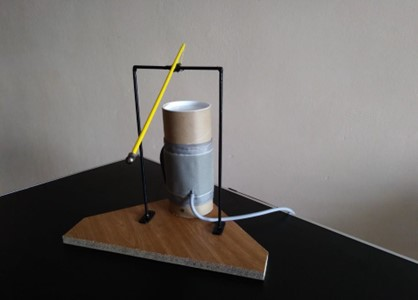
\includegraphics[width=1\textwidth]{pictures/mech_kyvadlo.jpg}
    \caption{Mechaniké kyvadlo pro vytvoření jednotkového impulsu na pneumatický systém.}
\end{figure}
\begin{figure}[H]
    \label{fig:pneu_impulse_response}
    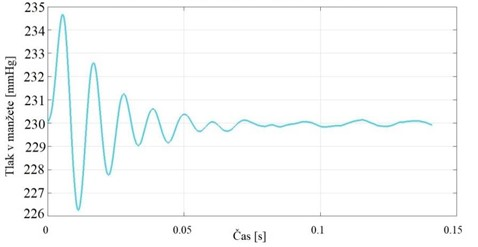
\includegraphics[width=1\textwidth]{pictures/pneu_impulse.jpg}
    \caption{Odezva pneumatického systému na jednotkový impuls.}
\end{figure}
Z naměřené hodnoty impulzní odezvy byly vypočteny parametry vlastní frekvence $f_0 \ [Hz]$ a poměrného útlumu $\xi \ [-]$. Pomocí těchto parametrů, za předpokladu, že se jedná o dynamický systém druhého řádu, bylo možné vypočítat přenosovou funkci systému.
\begin{figure}[H]
    \caption{Odezva pneumatického systému na jednotkový impuls.}
    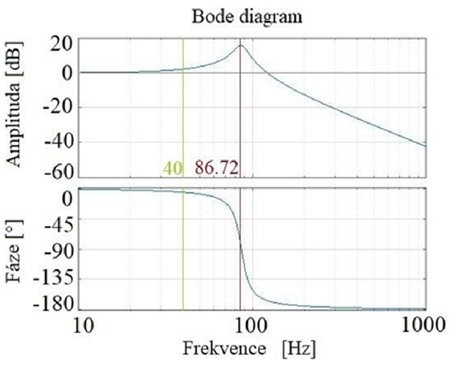
\includegraphics[width=1\textwidth]{pictures/freq_char_pneu.png}
    \label{fig:pneu_freq_char}
\end{figure}
Při měření srdečních frekvencí např. 120 tepů/min tj. 2 Hz, odpovídá 20. harmonická složka tepu frekvenci $f = 40 \ Hz$. Podle obrázku \ref{fig:pneu_freq_char} srdeční frekvence je amplituda zkreslena o +2 dB a fáze signálu o $^\circ 5$, což jsou akceptovatelné hodnoty.

%Conclusion


%% END

\chapter{Závěr}
Úkolem této bakalářské práce bylo provést rešerši přístrojů pro měření hemodynamických parametrů krevního řečiště určovaných neinvazivně z tvaru
tlakové křivky, navrhnout a realizovat systém pro snímání tlakových pulzací pomocí pažní manžety, vyhodnotit technické parametry a vytvořit technickou dokumentaci navrženého řešení.
\par
První část se věnovala popisu hemodynamických parametrů krevního řečiště, popsání metod měření parametrů a rešerši přístrojů pro měření hemodynamických parametrů krevního řečiště určovaných neinvazivně z tvaru
tlakové křivky.
\par
Druhá část byla zaměřena na návrh a dokumentaci systému pro snímání tlakových pulzací pomocí pažní manžety.
\par
Poslední část se poté věnovala popisu a charakterizaci parametrů navrženého systému, testům těsnosti pneumatické části, charakteristice analogově-digitálních převodníků pro tlakové sensory a měření pulzní tlakové křivky dobrovolníka.
\par
Výsledkem bakalářské práce je systém pro snímání tlakových pulzací pomocí pažní manžety, jeho dokumentace a popis parametrů. Systém dokáže ovládat ventily, umožňuje sběr dat z tlakových sensorů a ostatních periférií, jejich následné zpracování a komunikaci s nadřazeným systémem.
\par
Na realizovaném systému je potřeba dobudoucna zlepšit frekvenční odezvu filtru pro napájení analogové části mikroprocesoru, těsnost pneumatického systému. Další vylepšení se může zaměřit na analýzu rušení sensorů a jeho potlačení, zlepšení odolnosti proti elektromagnetickému rušení, vytvoření uživatelského prostředí, vytvoření vlastních knihoven pro
mikroprocesor STM32, dálkový upgrade firmware z uživatelského prostředí a vytvoření softwarového systému Board Support Package pro podporu více verzí desky plošného spoje jedním softwarem.
\par
Vytvořený systém splňuje požadavky zadání bakalářské práce. Systém je navržen, realizován, jsou popsané jeho parametry a je vytvořená jeho dokumentace.


\appendix

\printindex


\nocite{*}
% \bibliographystyle{amsalpha}
\bibliographystyle{plain}

\bibliography{main}
\chapter{Schéma DPS}
Následující stránky obsahují.
\begin{itemize}
	\item Schéma zapojení DPS
	\item Elektrické spoje zadní strany DPS
	\item Maska zadní strany DSP
	\item Elektrické spoje přední strany DSP
	\item Maska přední strany DSP
	\item Silkscreen přední strany DSP
	\item Druhá vrstva GND DPS
	\item Třetí vrstva 3V3 DPS
\end{itemize}

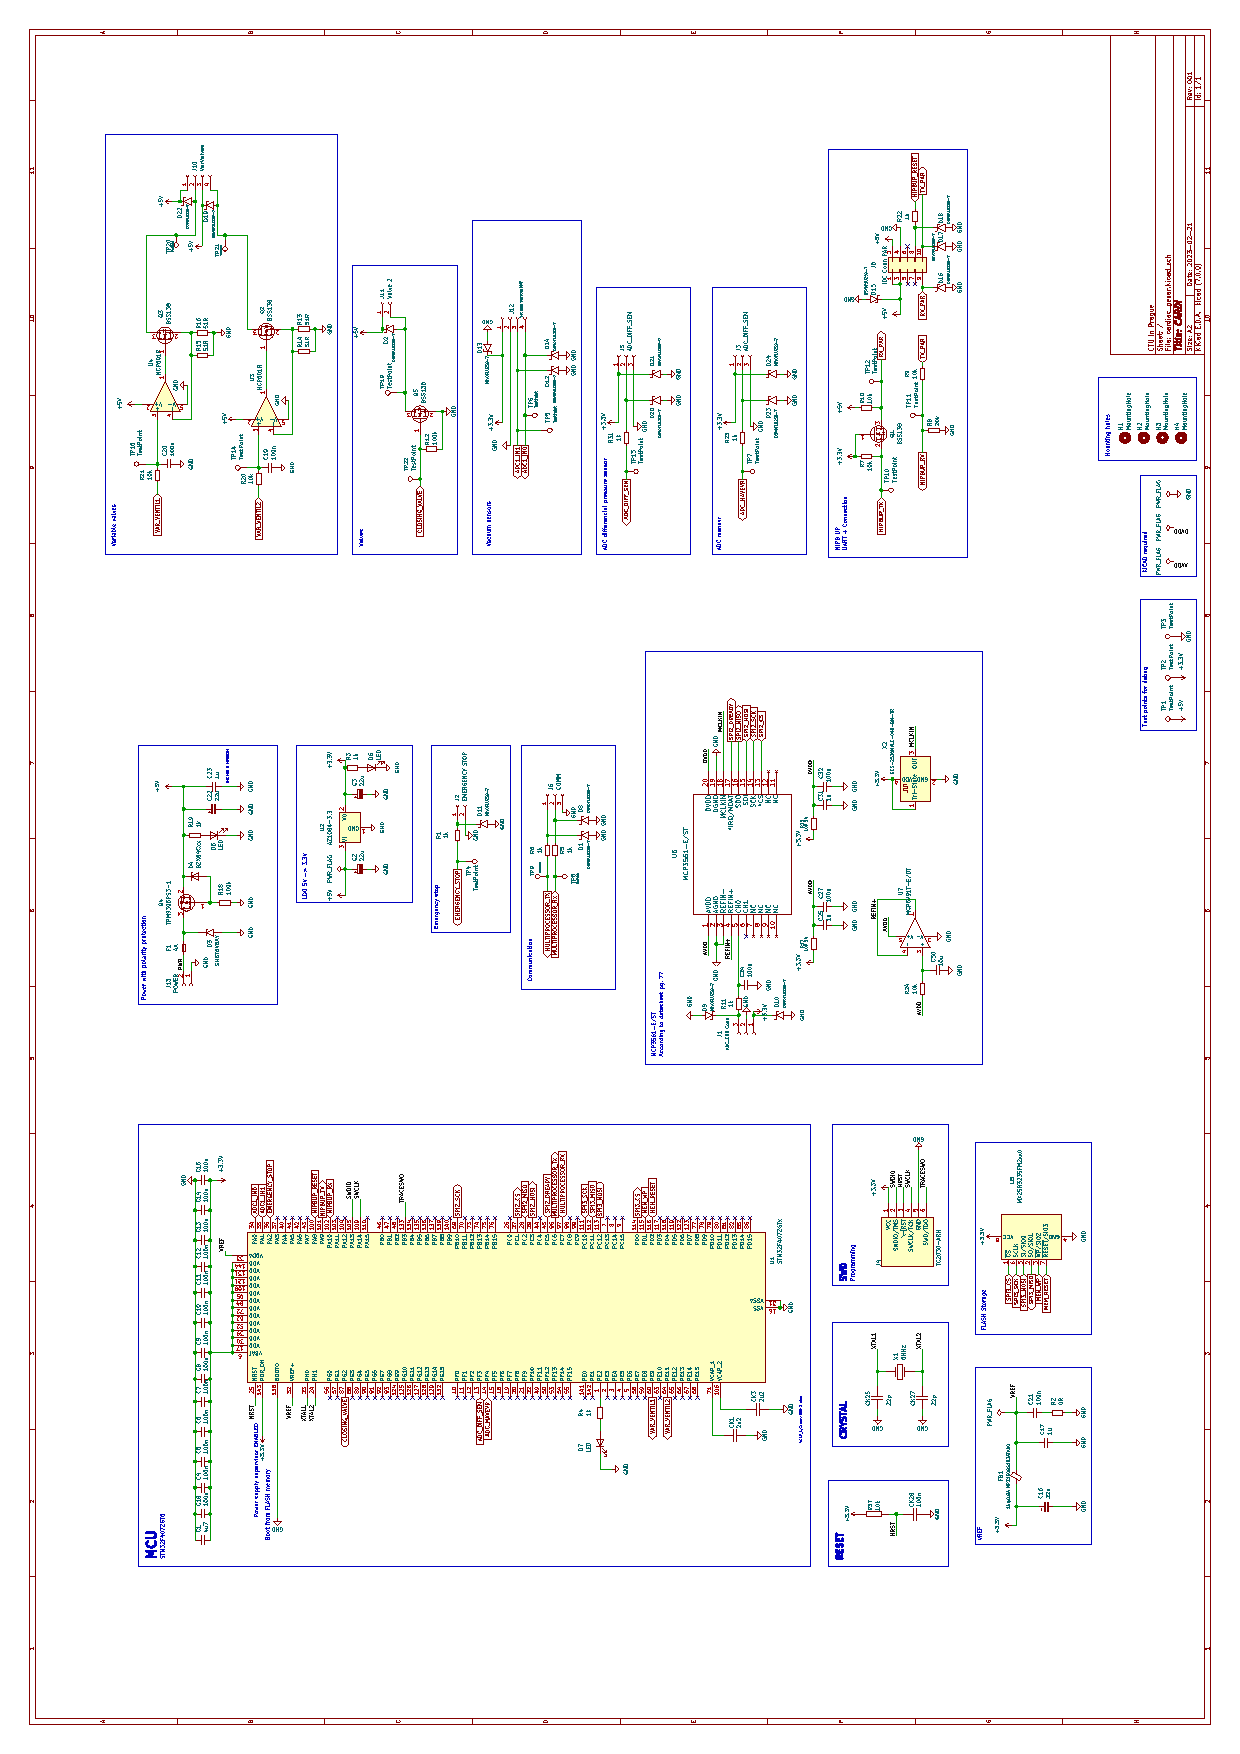
\includepdf{pictures/cardiac_gener.pdf}
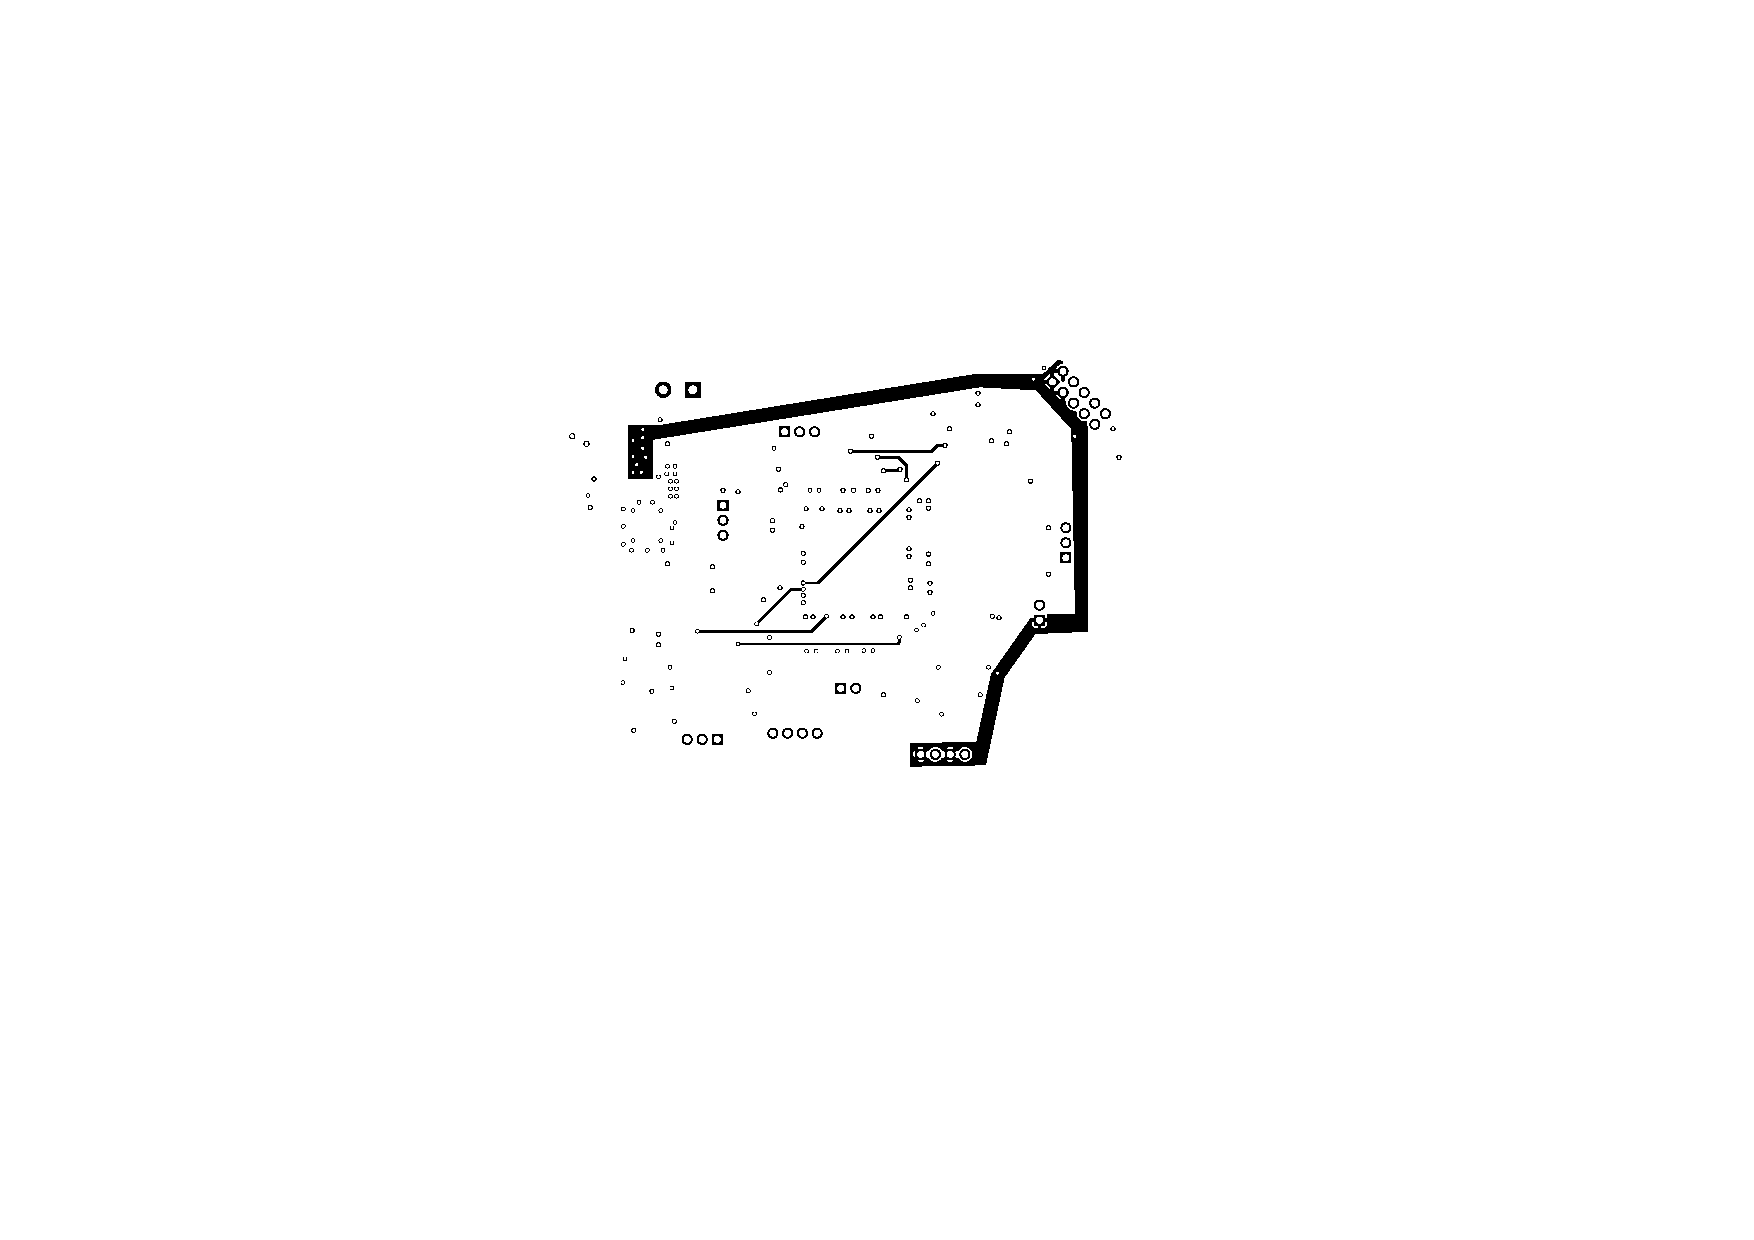
\includepdf{pictures/cardiac_gener-B_Cu.pdf}
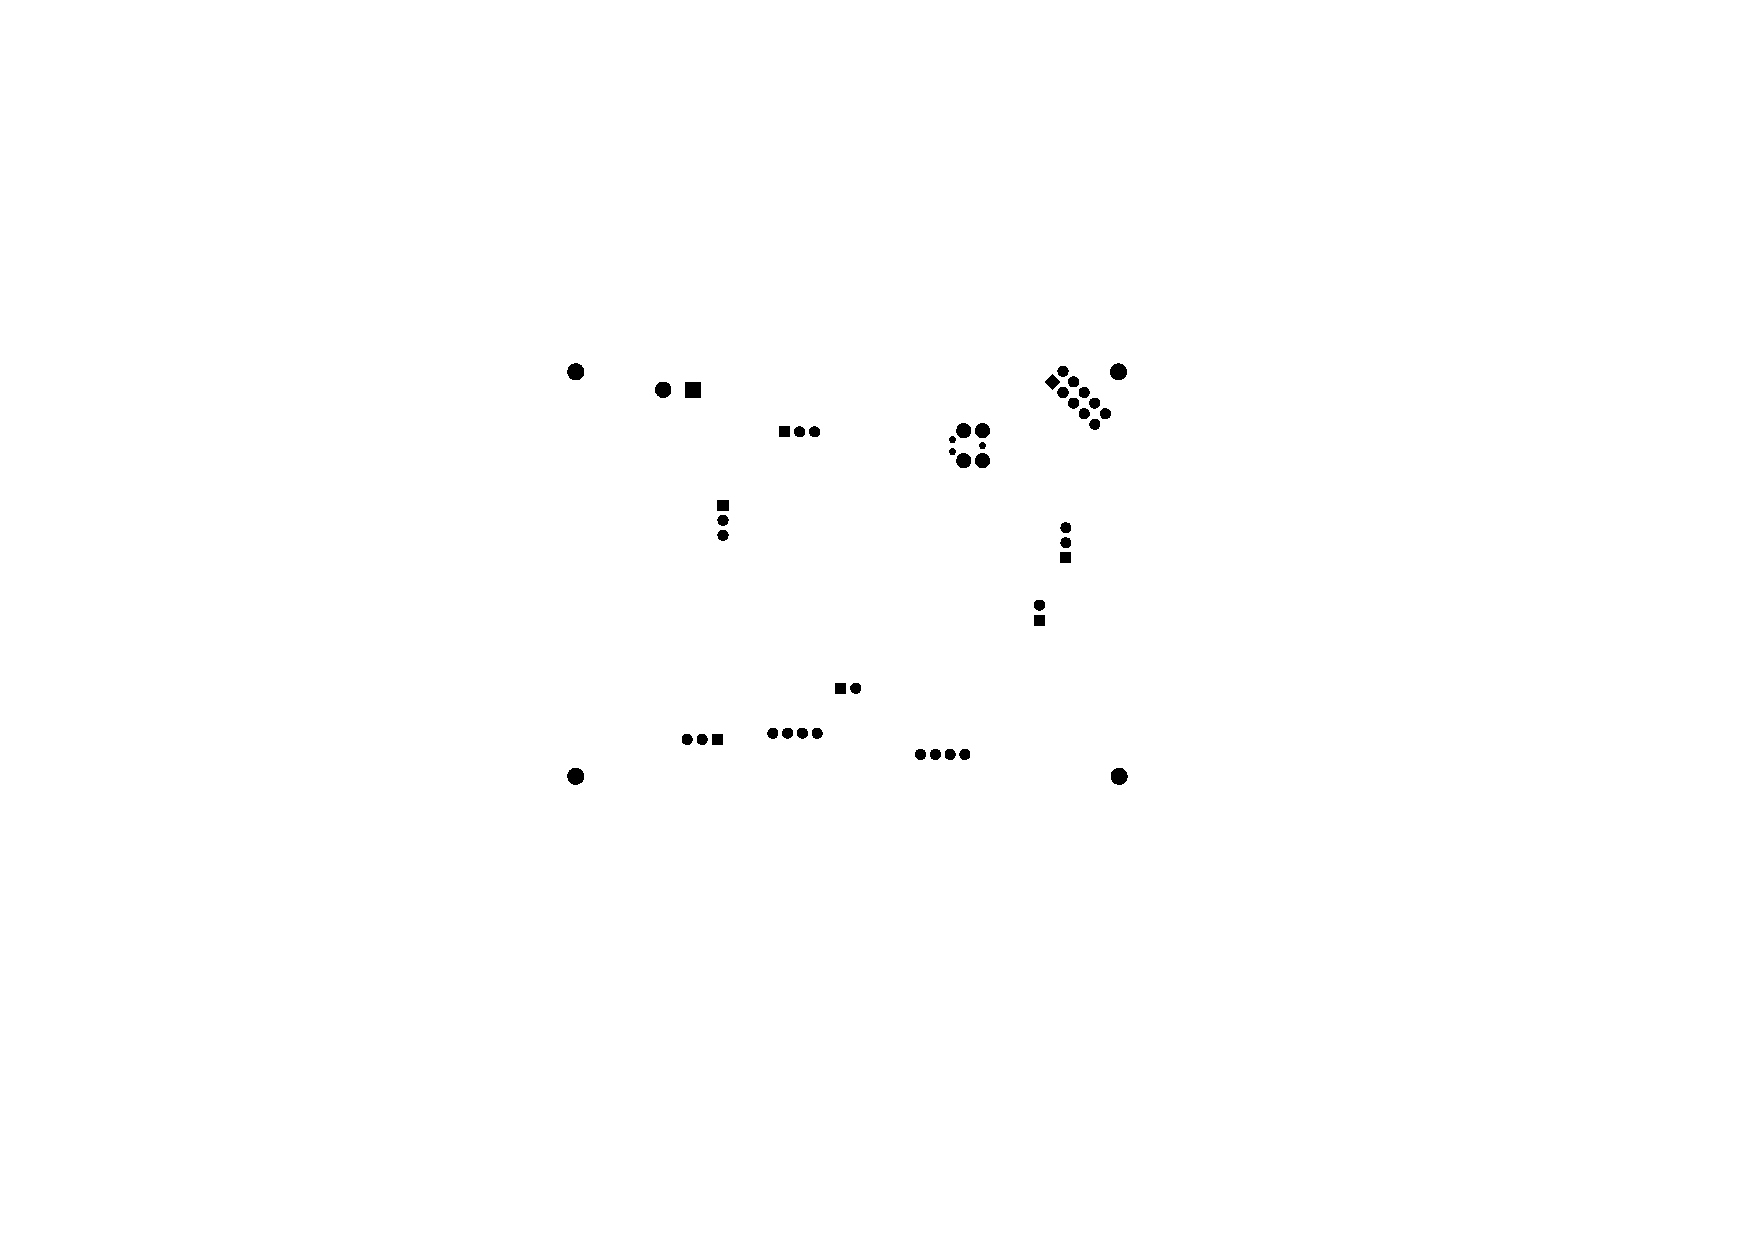
\includepdf{pictures/cardiac_gener-B_Mask.pdf}
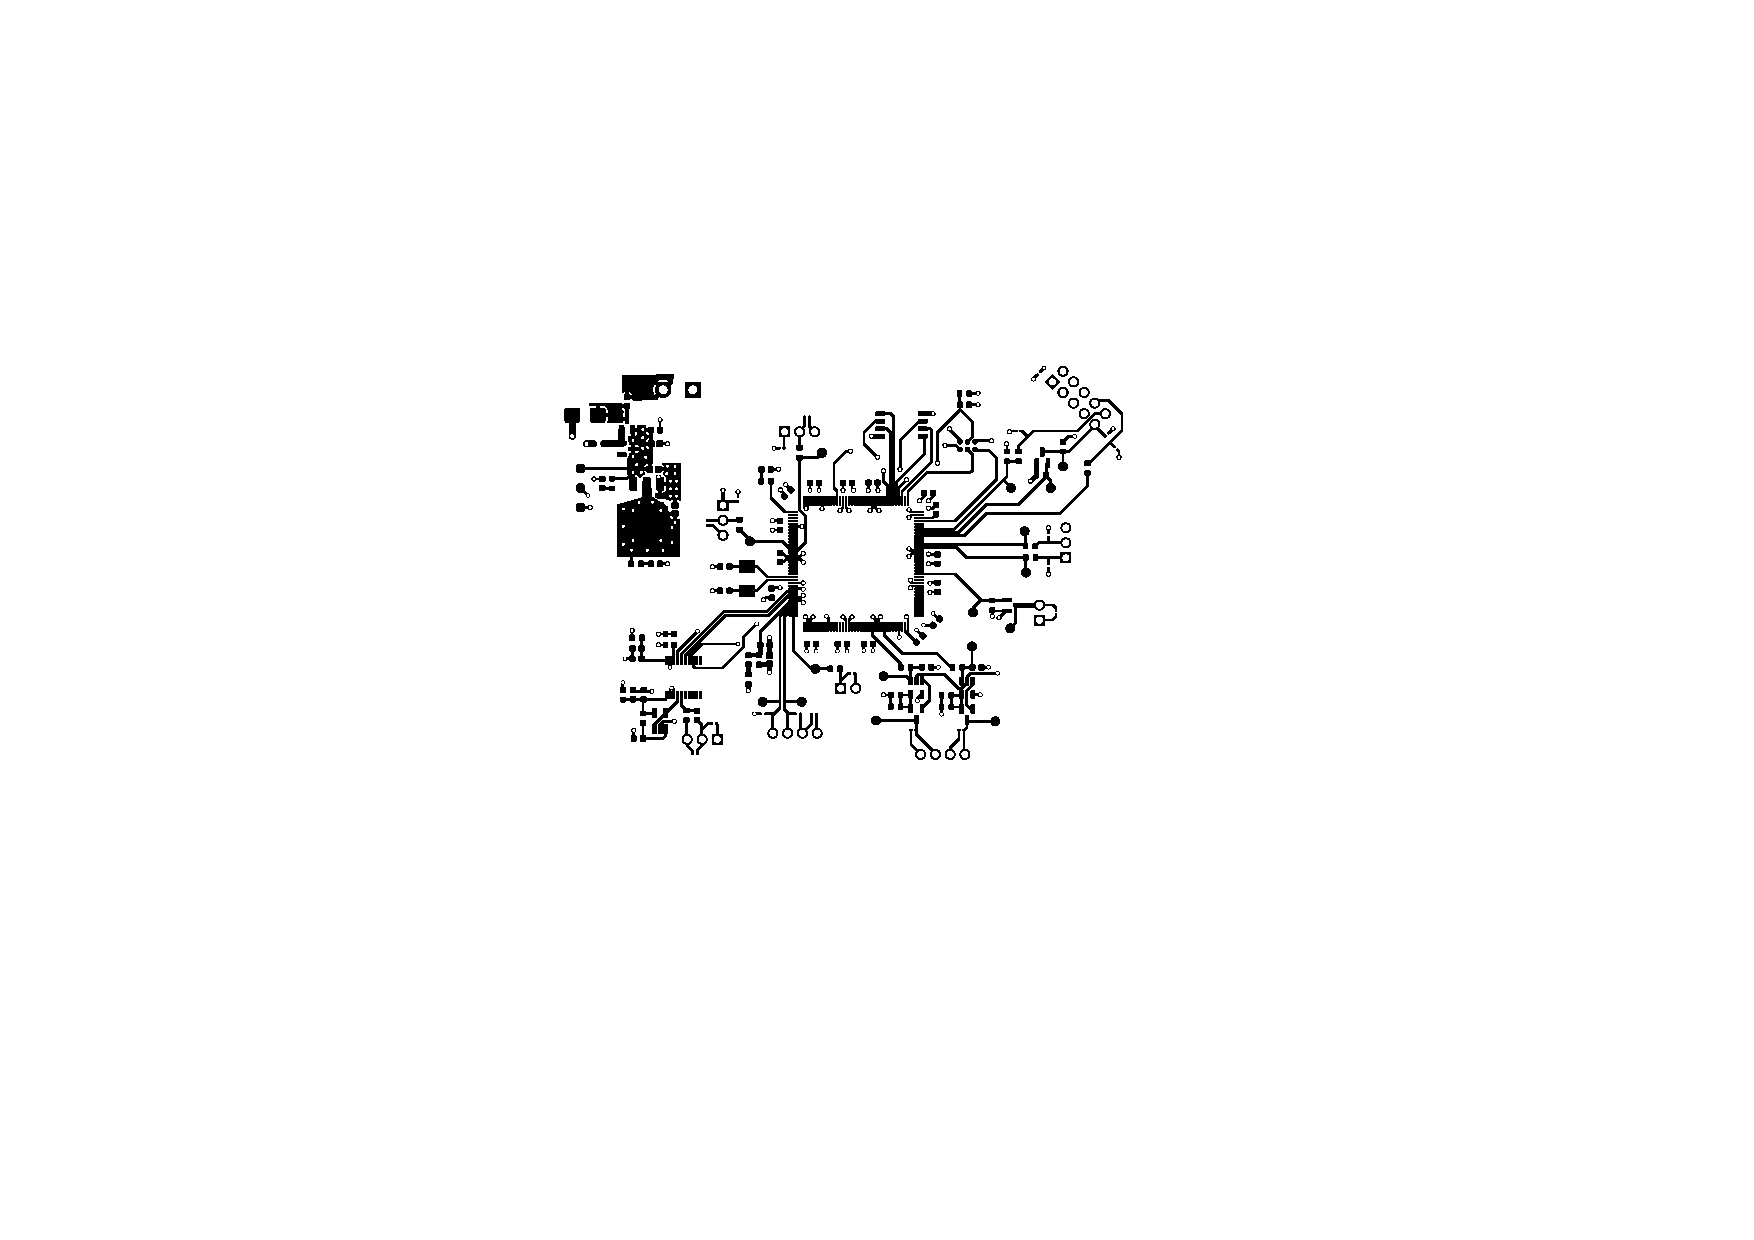
\includepdf{pictures/cardiac_gener-F_Cu.pdf}
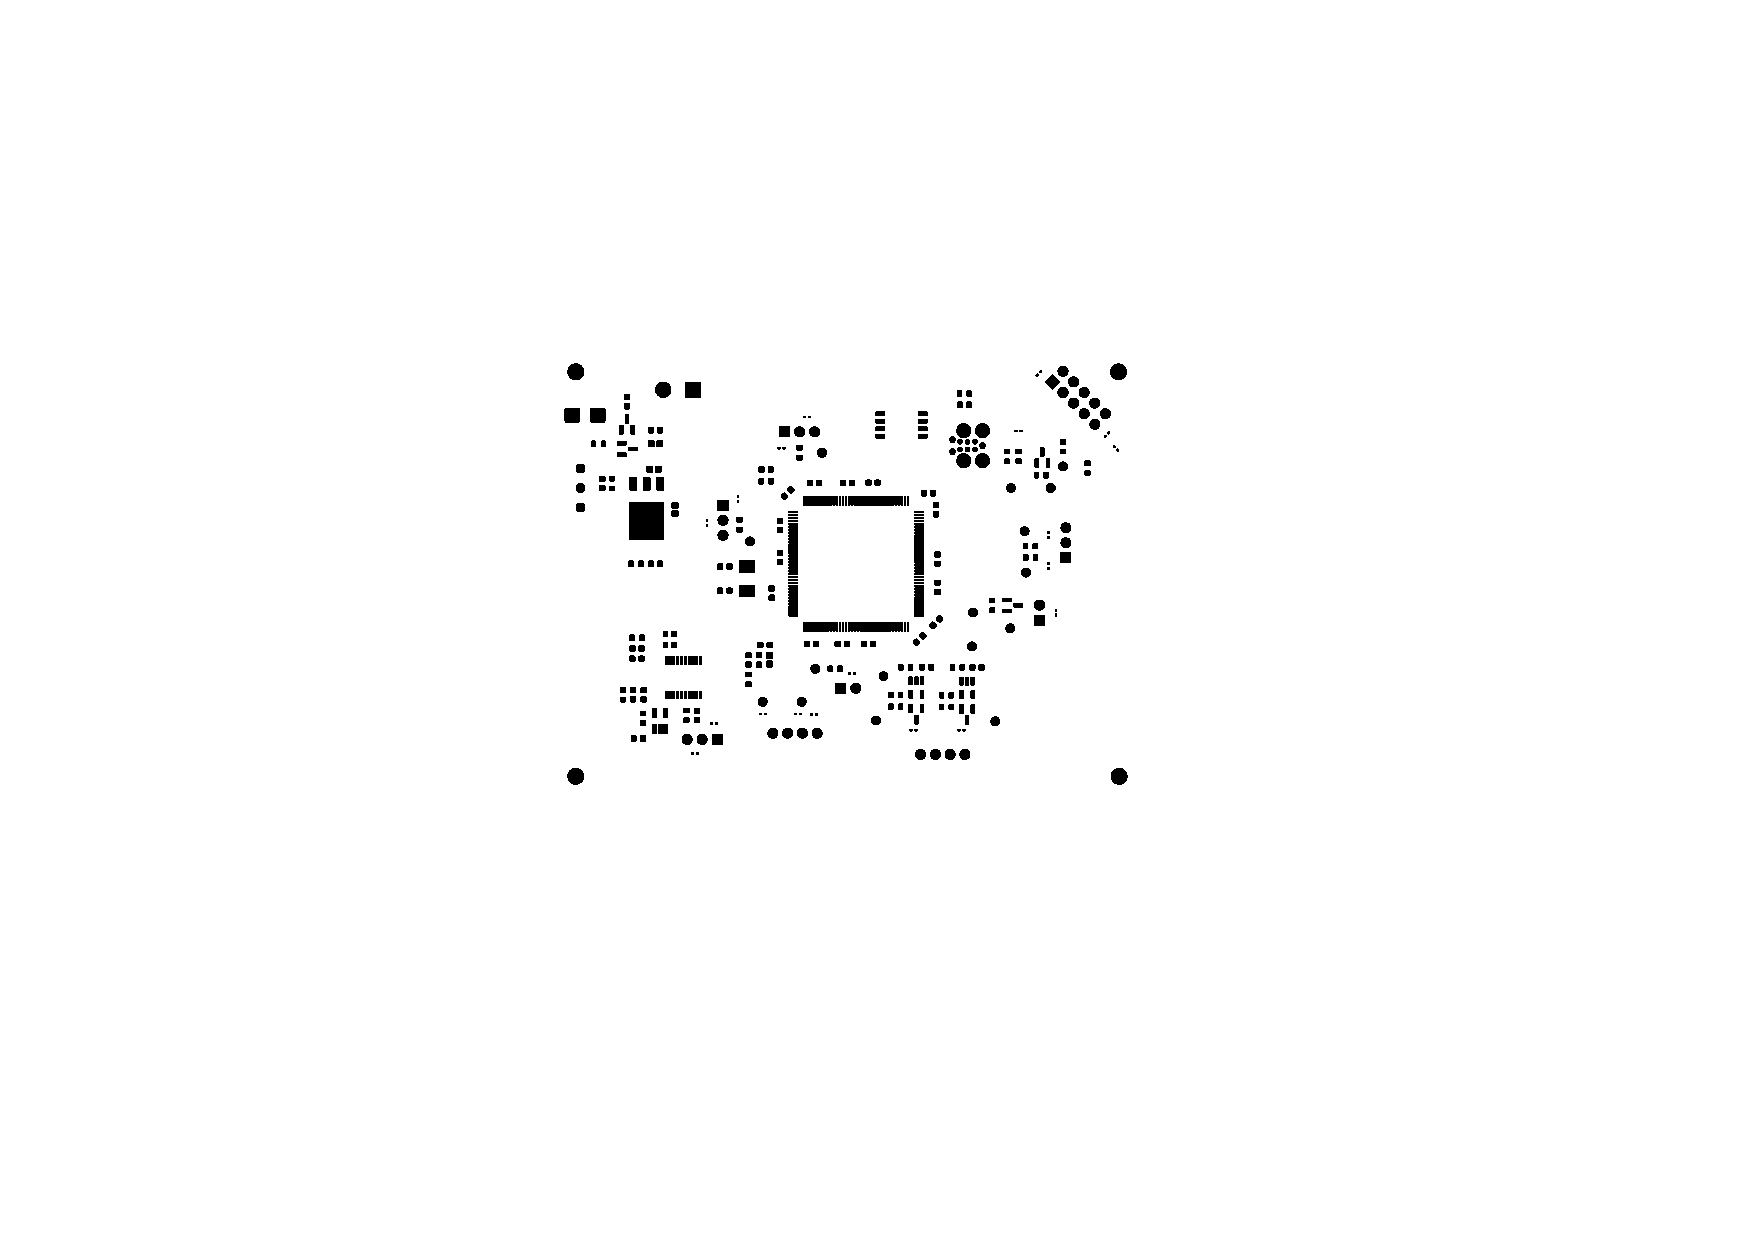
\includepdf{pictures/cardiac_gener-F_Mask.pdf}
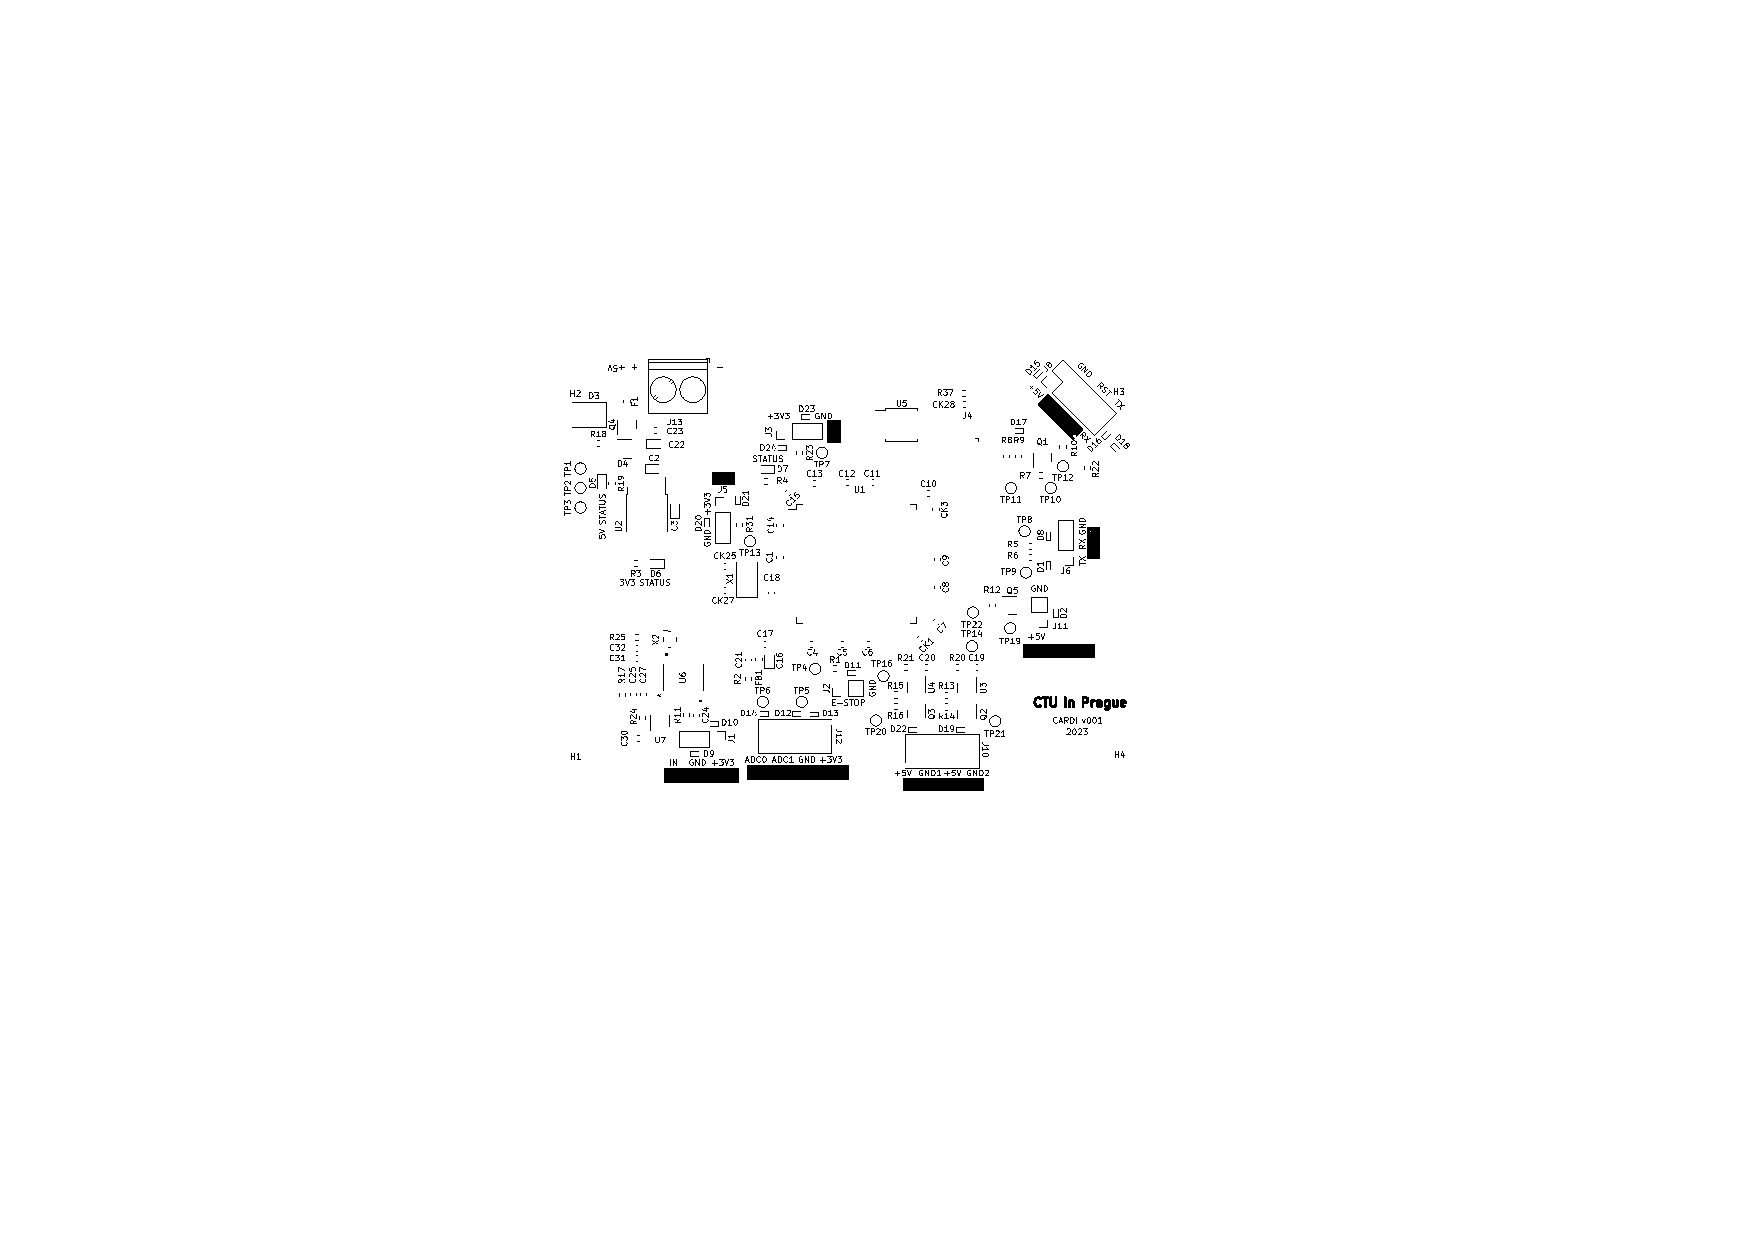
\includepdf{pictures/cardiac_gener-F_Silkscreen.pdf}
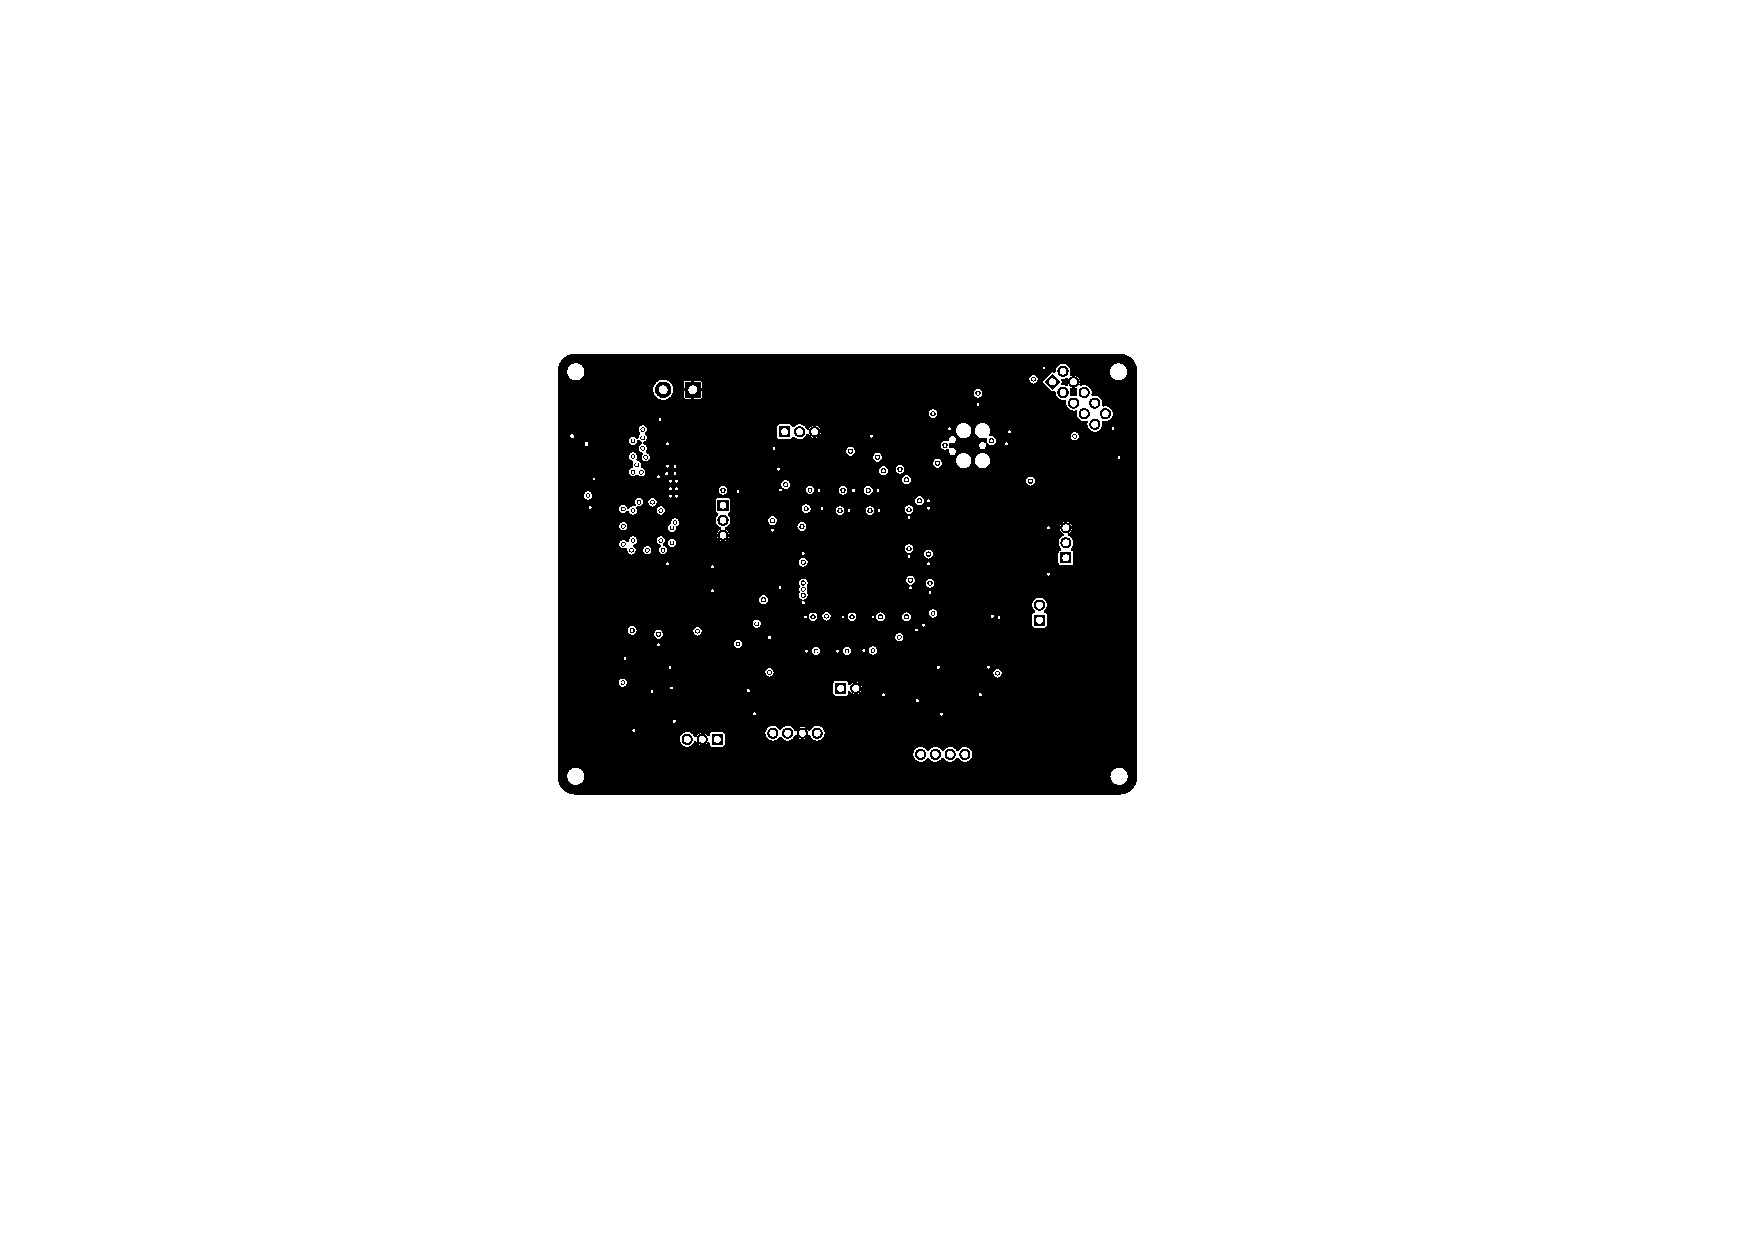
\includepdf{pictures/cardiac_gener-In1_GND_Cu.pdf}
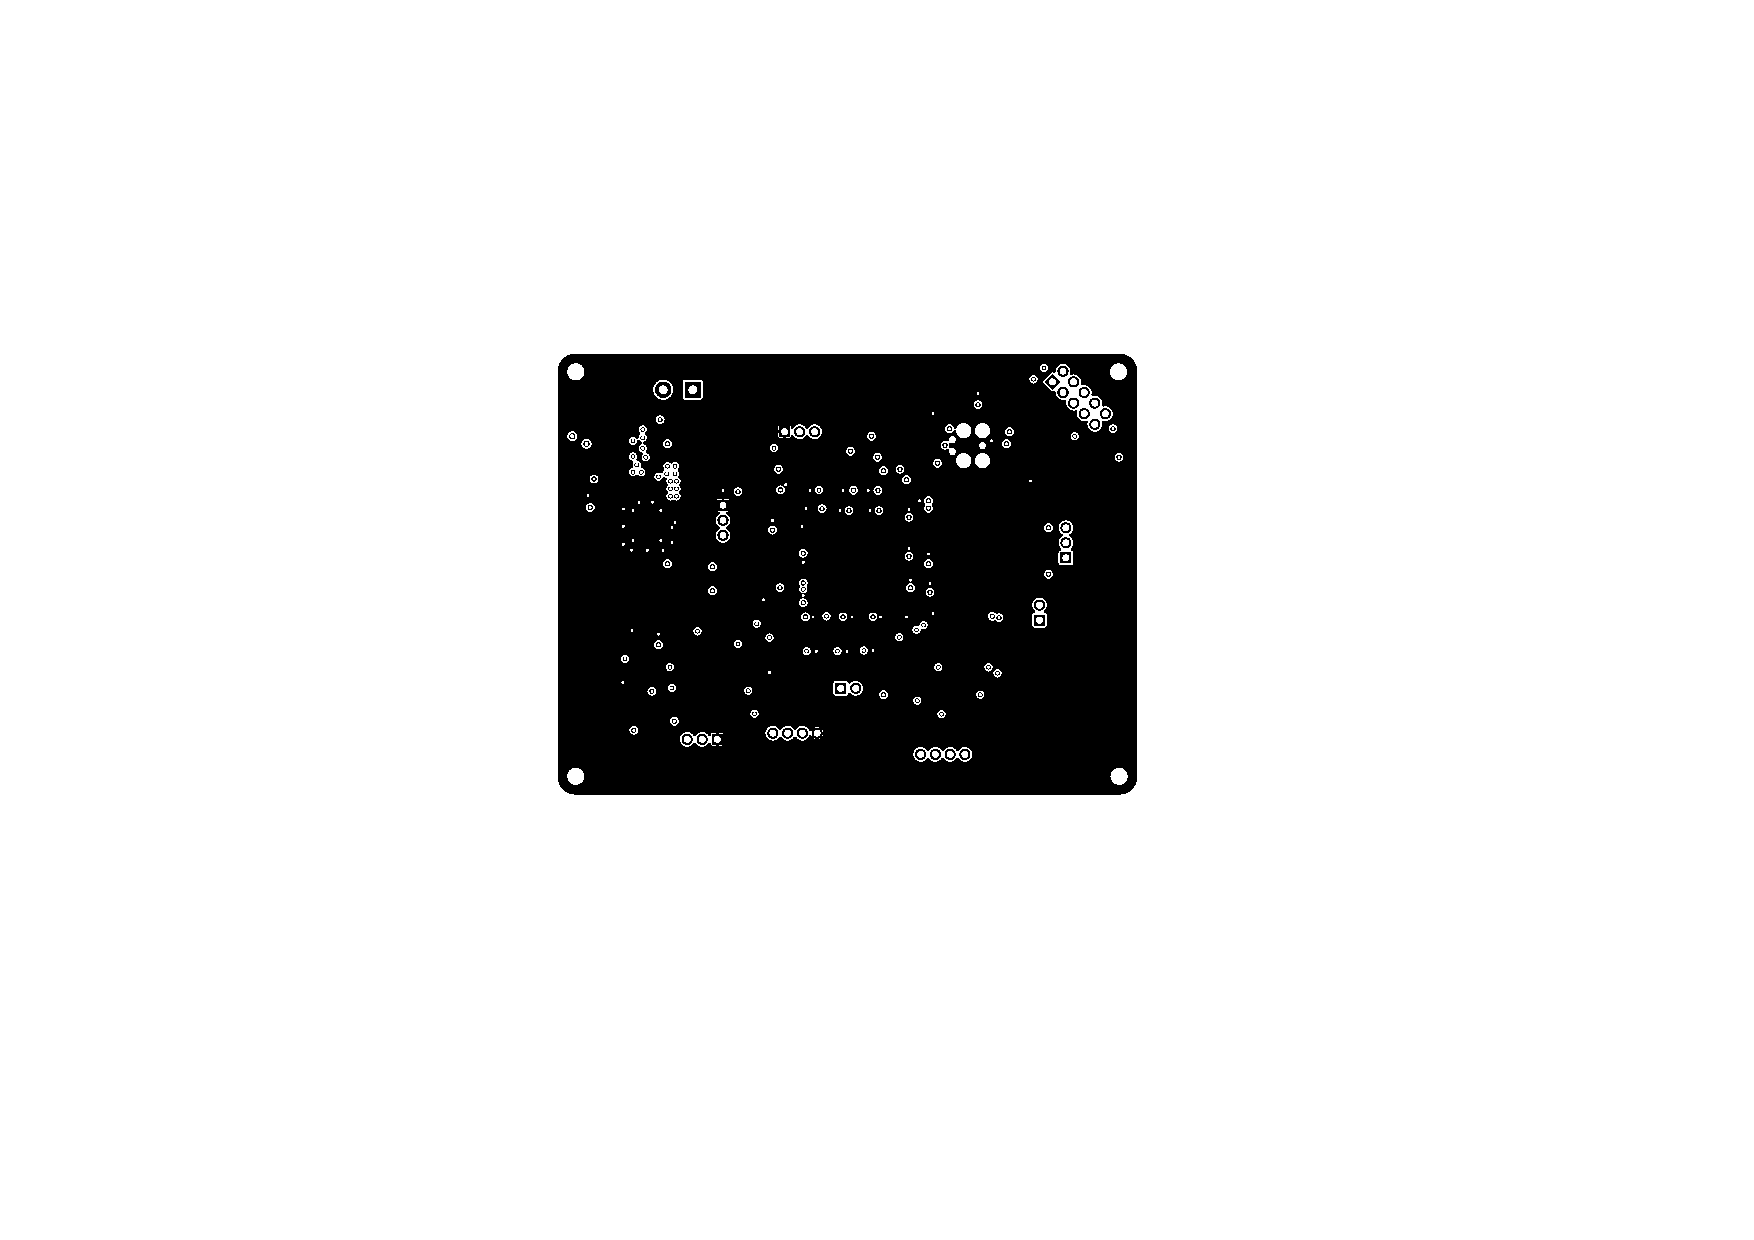
\includepdf{pictures/cardiac_gener-In2_3V3_Cu.pdf}

\end{document}